% Options for packages loaded elsewhere
% Options for packages loaded elsewhere
\PassOptionsToPackage{unicode}{hyperref}
\PassOptionsToPackage{hyphens}{url}
\PassOptionsToPackage{dvipsnames,svgnames,x11names}{xcolor}
%
\documentclass[
  english,
  letterpaper,
  DIV=11,
  numbers=noendperiod]{scrreprt}
\usepackage{xcolor}
\usepackage{amsmath,amssymb}
\setcounter{secnumdepth}{5}
\usepackage{iftex}
\ifPDFTeX
  \usepackage[T1]{fontenc}
  \usepackage[utf8]{inputenc}
  \usepackage{textcomp} % provide euro and other symbols
\else % if luatex or xetex
  \usepackage{unicode-math} % this also loads fontspec
  \defaultfontfeatures{Scale=MatchLowercase}
  \defaultfontfeatures[\rmfamily]{Ligatures=TeX,Scale=1}
\fi
\usepackage{lmodern}
\ifPDFTeX\else
  % xetex/luatex font selection
\fi
% Use upquote if available, for straight quotes in verbatim environments
\IfFileExists{upquote.sty}{\usepackage{upquote}}{}
\IfFileExists{microtype.sty}{% use microtype if available
  \usepackage[]{microtype}
  \UseMicrotypeSet[protrusion]{basicmath} % disable protrusion for tt fonts
}{}
\makeatletter
\@ifundefined{KOMAClassName}{% if non-KOMA class
  \IfFileExists{parskip.sty}{%
    \usepackage{parskip}
  }{% else
    \setlength{\parindent}{0pt}
    \setlength{\parskip}{6pt plus 2pt minus 1pt}}
}{% if KOMA class
  \KOMAoptions{parskip=half}}
\makeatother
% Make \paragraph and \subparagraph free-standing
\makeatletter
\ifx\paragraph\undefined\else
  \let\oldparagraph\paragraph
  \renewcommand{\paragraph}{
    \@ifstar
      \xxxParagraphStar
      \xxxParagraphNoStar
  }
  \newcommand{\xxxParagraphStar}[1]{\oldparagraph*{#1}\mbox{}}
  \newcommand{\xxxParagraphNoStar}[1]{\oldparagraph{#1}\mbox{}}
\fi
\ifx\subparagraph\undefined\else
  \let\oldsubparagraph\subparagraph
  \renewcommand{\subparagraph}{
    \@ifstar
      \xxxSubParagraphStar
      \xxxSubParagraphNoStar
  }
  \newcommand{\xxxSubParagraphStar}[1]{\oldsubparagraph*{#1}\mbox{}}
  \newcommand{\xxxSubParagraphNoStar}[1]{\oldsubparagraph{#1}\mbox{}}
\fi
\makeatother

\usepackage{color}
\usepackage{fancyvrb}
\newcommand{\VerbBar}{|}
\newcommand{\VERB}{\Verb[commandchars=\\\{\}]}
\DefineVerbatimEnvironment{Highlighting}{Verbatim}{commandchars=\\\{\}}
% Add ',fontsize=\small' for more characters per line
\usepackage{framed}
\definecolor{shadecolor}{RGB}{241,243,245}
\newenvironment{Shaded}{\begin{snugshade}}{\end{snugshade}}
\newcommand{\AlertTok}[1]{\textcolor[rgb]{0.68,0.00,0.00}{#1}}
\newcommand{\AnnotationTok}[1]{\textcolor[rgb]{0.37,0.37,0.37}{#1}}
\newcommand{\AttributeTok}[1]{\textcolor[rgb]{0.40,0.45,0.13}{#1}}
\newcommand{\BaseNTok}[1]{\textcolor[rgb]{0.68,0.00,0.00}{#1}}
\newcommand{\BuiltInTok}[1]{\textcolor[rgb]{0.00,0.23,0.31}{#1}}
\newcommand{\CharTok}[1]{\textcolor[rgb]{0.13,0.47,0.30}{#1}}
\newcommand{\CommentTok}[1]{\textcolor[rgb]{0.37,0.37,0.37}{#1}}
\newcommand{\CommentVarTok}[1]{\textcolor[rgb]{0.37,0.37,0.37}{\textit{#1}}}
\newcommand{\ConstantTok}[1]{\textcolor[rgb]{0.56,0.35,0.01}{#1}}
\newcommand{\ControlFlowTok}[1]{\textcolor[rgb]{0.00,0.23,0.31}{\textbf{#1}}}
\newcommand{\DataTypeTok}[1]{\textcolor[rgb]{0.68,0.00,0.00}{#1}}
\newcommand{\DecValTok}[1]{\textcolor[rgb]{0.68,0.00,0.00}{#1}}
\newcommand{\DocumentationTok}[1]{\textcolor[rgb]{0.37,0.37,0.37}{\textit{#1}}}
\newcommand{\ErrorTok}[1]{\textcolor[rgb]{0.68,0.00,0.00}{#1}}
\newcommand{\ExtensionTok}[1]{\textcolor[rgb]{0.00,0.23,0.31}{#1}}
\newcommand{\FloatTok}[1]{\textcolor[rgb]{0.68,0.00,0.00}{#1}}
\newcommand{\FunctionTok}[1]{\textcolor[rgb]{0.28,0.35,0.67}{#1}}
\newcommand{\ImportTok}[1]{\textcolor[rgb]{0.00,0.46,0.62}{#1}}
\newcommand{\InformationTok}[1]{\textcolor[rgb]{0.37,0.37,0.37}{#1}}
\newcommand{\KeywordTok}[1]{\textcolor[rgb]{0.00,0.23,0.31}{\textbf{#1}}}
\newcommand{\NormalTok}[1]{\textcolor[rgb]{0.00,0.23,0.31}{#1}}
\newcommand{\OperatorTok}[1]{\textcolor[rgb]{0.37,0.37,0.37}{#1}}
\newcommand{\OtherTok}[1]{\textcolor[rgb]{0.00,0.23,0.31}{#1}}
\newcommand{\PreprocessorTok}[1]{\textcolor[rgb]{0.68,0.00,0.00}{#1}}
\newcommand{\RegionMarkerTok}[1]{\textcolor[rgb]{0.00,0.23,0.31}{#1}}
\newcommand{\SpecialCharTok}[1]{\textcolor[rgb]{0.37,0.37,0.37}{#1}}
\newcommand{\SpecialStringTok}[1]{\textcolor[rgb]{0.13,0.47,0.30}{#1}}
\newcommand{\StringTok}[1]{\textcolor[rgb]{0.13,0.47,0.30}{#1}}
\newcommand{\VariableTok}[1]{\textcolor[rgb]{0.07,0.07,0.07}{#1}}
\newcommand{\VerbatimStringTok}[1]{\textcolor[rgb]{0.13,0.47,0.30}{#1}}
\newcommand{\WarningTok}[1]{\textcolor[rgb]{0.37,0.37,0.37}{\textit{#1}}}

\usepackage{longtable,booktabs,array}
\newcounter{none} % for unnumbered tables
\usepackage{calc} % for calculating minipage widths
% Correct order of tables after \paragraph or \subparagraph
\usepackage{etoolbox}
\makeatletter
\patchcmd\longtable{\par}{\if@noskipsec\mbox{}\fi\par}{}{}
\makeatother
% Allow footnotes in longtable head/foot
\IfFileExists{footnotehyper.sty}{\usepackage{footnotehyper}}{\usepackage{footnote}}
\makesavenoteenv{longtable}
\usepackage{graphicx}
\makeatletter
\newsavebox\pandoc@box
\newcommand*\pandocbounded[1]{% scales image to fit in text height/width
  \sbox\pandoc@box{#1}%
  \Gscale@div\@tempa{\textheight}{\dimexpr\ht\pandoc@box+\dp\pandoc@box\relax}%
  \Gscale@div\@tempb{\linewidth}{\wd\pandoc@box}%
  \ifdim\@tempb\p@<\@tempa\p@\let\@tempa\@tempb\fi% select the smaller of both
  \ifdim\@tempa\p@<\p@\scalebox{\@tempa}{\usebox\pandoc@box}%
  \else\usebox{\pandoc@box}%
  \fi%
}
% Set default figure placement to htbp
\def\fps@figure{htbp}
\makeatother



\ifLuaTeX
\usepackage[bidi=basic,shorthands=off]{babel}
\else
\usepackage[bidi=default,shorthands=off]{babel}
\fi
\ifLuaTeX
  \usepackage{selnolig} % disable illegal ligatures
\fi


\setlength{\emergencystretch}{3em} % prevent overfull lines

\providecommand{\tightlist}{%
  \setlength{\itemsep}{0pt}\setlength{\parskip}{0pt}}



 


\KOMAoption{captions}{tableheading}
\titlehead{
\includegraphics[width=6in]{aiwd.jpg}}
\makeatletter
\@ifpackageloaded{caption}{}{\usepackage{caption}}
\AtBeginDocument{%
\ifdefined\contentsname
  \renewcommand*\contentsname{Table of contents}
\else
  \newcommand\contentsname{Table of contents}
\fi
\ifdefined\listfigurename
  \renewcommand*\listfigurename{List of Figures}
\else
  \newcommand\listfigurename{List of Figures}
\fi
\ifdefined\listtablename
  \renewcommand*\listtablename{List of Tables}
\else
  \newcommand\listtablename{List of Tables}
\fi
\ifdefined\figurename
  \renewcommand*\figurename{Figure}
\else
  \newcommand\figurename{Figure}
\fi
\ifdefined\tablename
  \renewcommand*\tablename{Table}
\else
  \newcommand\tablename{Table}
\fi
}
\@ifpackageloaded{float}{}{\usepackage{float}}
\floatstyle{ruled}
\@ifundefined{c@chapter}{\newfloat{codelisting}{h}{lop}}{\newfloat{codelisting}{h}{lop}[chapter]}
\floatname{codelisting}{Listing}
\newcommand*\listoflistings{\listof{codelisting}{List of Listings}}
\makeatother
\makeatletter
\makeatother
\makeatletter
\@ifpackageloaded{caption}{}{\usepackage{caption}}
\@ifpackageloaded{subcaption}{}{\usepackage{subcaption}}
\makeatother
\makeatletter
\@ifpackageloaded{tikz}{}{\usepackage{tikz}}
\makeatother
        \newcommand*\circled[1]{\tikz[baseline=(char.base)]{
          \node[shape=circle,draw,inner sep=1pt] (char) {{\scriptsize#1}};}}  
                  
\usepackage{bookmark}
\IfFileExists{xurl.sty}{\usepackage{xurl}}{} % add URL line breaks if available
\urlstyle{same}
\hypersetup{
  pdftitle={Data analysis and visualisation},
  pdfauthor={Piotr Jastrzębski},
  pdflang={en},
  colorlinks=true,
  linkcolor={blue},
  filecolor={Maroon},
  citecolor={Blue},
  urlcolor={Blue},
  pdfcreator={LaTeX via pandoc}}


\title{Data analysis and visualisation}
\author{Piotr Jastrzębski}
\date{2026-05-03}
\begin{document}
\maketitle

\renewcommand*\contentsname{Table of contents}
{
\setcounter{tocdepth}{2}
\tableofcontents
}

\chapter{Data Analysis and
Visualization}\label{data-analysis-and-visualization}

The current version pertains to classes held in the 2025/26 academic
year.

\emph{Some of the texts have been machine-translated into English. In
case of any ambiguities, please get in touch via email.}

\part{Introduction}

\chapter{A bit of theory\ldots{}}\label{a-bit-of-theory}

\section{Rational thinking test}\label{rational-thinking-test}

\begin{itemize}
\tightlist
\item
  If 5 machines produce 5 devices in 5 minutes, how long will it take
  100 machines to make 100 devices?
\item
  A patch of water lilies is growing on a pond. Every day the patch
  doubles in size. If it takes 48 days for the lilies to cover the
  entire pond, how many days does it take for them to cover half the
  pond?
\item
  A baseball bat and a ball cost \$1.10 together. The bat costs one
  dollar more than the ball. How much does the ball cost?
\end{itemize}

\section{Data analysis}\label{data-analysis}

Data analysis is the process of examining, cleaning, transforming, and
modeling data in order to discover useful information, draw conclusions,
and support decision-making. It is a multi-stage process that includes:

\begin{itemize}
\tightlist
\item
  Collecting data from various sources
\item
  Cleaning data by removing errors, missing values, and inconsistencies
\item
  Exploring data to understand its structure and characteristics
\item
  Transforming data into the appropriate format
\item
  Applying statistical methods and machine learning algorithms
\item
  Interpreting results in the context of a specific business or
  scientific problem
\end{itemize}

Data analysis is used in nearly every field, from business and finance
to social sciences, medicine, and scientific research. The goal of data
analysis is to transform raw data into knowledge that can be used to
make better decisions.

\section{Data visualization}\label{data-visualization}

Data visualization is the graphical representation of information and
data. It uses visual elements such as charts, maps, and dashboards to
present relationships between data in a way that is easy to understand
and interpret. Good data visualization:

\begin{itemize}
\tightlist
\item
  Presents complex information in an accessible and intuitive way
\item
  Reveals patterns, trends, and outliers that may be difficult to notice
  in raw data
\item
  Supports the data analysis process by enabling quick review of large
  datasets
\item
  Facilitates communication of analysis results to various audiences,
  including non-technical individuals
\item
  Helps tell stories contained in data (data storytelling)
\end{itemize}

The most popular types of data visualization include bar charts, line
charts, pie charts, heatmaps, hierarchical trees, word clouds, and
interactive dashboards. The choice of the appropriate visualization form
depends on the type of data, the purpose of the presentation, and the
target audience.

Data visualization is a key element of the data analysis process because
it allows for quick drawing of conclusions and making decisions based on
data. It is a bridge between complex data and human understanding.

\section{Data analysis - basic
concepts}\label{data-analysis---basic-concepts}

\subsection{Modern meanings of the word
``statistics'':}\label{modern-meanings-of-the-word-statistics}

\begin{itemize}
\tightlist
\item
  a set of numerical data showing the development of processes and
  phenomena, e.g.~population statistics.
\item
  all activities related to collecting and processing numerical data,
  e.g.~statistics on a certain problem conducted by the Central
  Statistical Office.
\item
  numerical characteristics, e.g.~sample statistics such as arithmetic
  mean, standard deviation, etc.
\item
  a scientific discipline - the science of methods for studying mass
  phenomena.
\end{itemize}

\subsection{``Massiveness''}\label{massiveness}

Mass phenomena/processes - a large number of units are subject to study.
They are divided into:

\begin{itemize}
\tightlist
\item
  economic (e.g.~production, consumption, services, advertising),
\item
  social (e.g.~traffic accidents, political views),
\item
  demographic (e.g.~births, aging, migrations).
\end{itemize}

\subsection{Division of statistics}\label{division-of-statistics}

Statistics - a scientific discipline - division:

\begin{itemize}
\tightlist
\item
  descriptive statistics - deals with matters related to collecting,
  presenting, analyzing, and interpreting numerical data. Observation
  covers the entire population under study.
\item
  mathematical statistics - generalization of the results of studying a
  part of the population (sample) to the entire population.
\end{itemize}

\subsection{Population}\label{population}

Statistical population: a set of objects subject to statistical study.
It consists of units that are similar to each other, logically related,
but not identical. They share certain common features and certain
properties that allow them to be differentiated.

\begin{itemize}
\tightlist
\item
  examples:

  \begin{itemize}
  \tightlist
  \item
    study of the height of Polish citizens - inhabitants of Poland
  \item
    level of education in schools of the Warmian-Masurian Voivodeship -
    schools of the Warmian-Masurian Voivodeship.
  \end{itemize}
\item
  division:

  \begin{itemize}
  \tightlist
  \item
    general population - covers the entirety,
  \item
    sample population (sample) - covers a part of the population.
  \end{itemize}
\end{itemize}

\subsection{Statistical unit}\label{statistical-unit}

Statistical unit: each element of a statistical population.

\begin{itemize}
\tightlist
\item
  examples:

  \begin{itemize}
  \tightlist
  \item
    UWM students - a UWM student
  \item
    inhabitants of Poland - every person living in Poland
  \item
    machines produced in a factory - every machine
  \end{itemize}
\end{itemize}

\subsection{Statistical features}\label{statistical-features}

Statistical features

\begin{itemize}
\tightlist
\item
  properties characterizing statistical units in a given statistical
  population.
\item
  they are divided into constant and variable.
\end{itemize}

Constant features

\begin{itemize}
\tightlist
\item
  properties that are common to all units of a given statistical
  population.
\item
  division:

  \begin{itemize}
  \tightlist
  \item
    substantive - who or what is the subject of the statistical study,
  \item
    temporal - when the study was conducted or what time period the
    study covers,
  \item
    spatial - what territory (place or area) the study concerns.
  \end{itemize}
\item
  example: students of the Faculty of Mathematics and Computer Science
  (WMiI) at UWM in Olsztyn in the academic year 2017/2018:

  \begin{itemize}
  \tightlist
  \item
    substantive feature: possession of a student ID card,
  \item
    temporal feature - students studying in the academic year 2017/2018,
  \item
    spatial feature - location: WMiI UWM in Olsztyn.
  \end{itemize}
\end{itemize}

Variable features

\begin{itemize}
\tightlist
\item
  properties that differentiate statistical units in a given population.
\item
  example: UWM students - variable features: age, sex, type of secondary
  school completed, eye color, height.
\end{itemize}

Important:

\begin{itemize}
\tightlist
\item
  only variable features are subject to observation,
\item
  a constant feature in one population may be a variable feature in
  another population.
\end{itemize}

Example: UWM students have an ID card issued by UWM. Students of all
universities in Poland have ID cards issued by different institutions.

\textbf{Division of variable features:}

\begin{itemize}
\tightlist
\item
  measurable (quantitative) features - can be expressed as a number with
  a specific unit of measurement.
\item
  non-measurable (qualitative) features - described verbally,
  representing certain categories.
\end{itemize}

Example: student population. Measurable features: age, weight, height,
number of absences. Non-measurable features: sex, eye color, field of
study.

For practical reasons, numerical codes are often assigned to
non-measurable features. However, they should not be confused with
measurable features. E.g. 1 - primary education, 2 - vocational
education, etc.

\textbf{Division of measurable features:}

\begin{itemize}
\tightlist
\item
  continuous - can take any value within a defined interval,
  e.g.~height, age, apartment area.
\item
  discrete - can take specific (discrete) numerical values without
  intermediate values, e.g.~number of people in a household, number of
  employees in a given company.
\end{itemize}

Discrete features usually have integer values, although this is not
always required, e.g.~the number of full-time positions in a company
(including part-time positions).

\subsection{Scales}\label{scales}

\textbf{Measurement scale}

\begin{itemize}
\tightlist
\item
  a system that allows the results of statistical measurements to be
  organized in a certain way.
\item
  division:

  \begin{itemize}
  \tightlist
  \item
    nominal scale,
  \item
    ordinal scale,
  \item
    interval scale,
  \item
    ratio scale.
  \end{itemize}
\end{itemize}

\textbf{Nominal scale}

\begin{itemize}
\tightlist
\item
  a scale in which a statistical unit is classified into a specific
  category.
\item
  values in this scale have no ordering.
\item
  example:
\end{itemize}

{\def\LTcaptype{none} % do not increment counter
\begin{longtable}[]{@{}ll@{}}
\toprule\noalign{}
Religion & Code \\
\midrule\noalign{}
\endhead
\bottomrule\noalign{}
\endlastfoot
Christianity & 1 \\
Islam & 2 \\
Buddhism & 3 \\
\end{longtable}
}

\textbf{Ordinal scale}

\begin{itemize}
\tightlist
\item
  values have a clearly defined order, but distances between them are
  not given,
\item
  allows elements to be ranked.
\item
  examples:
\end{itemize}

{\def\LTcaptype{none} % do not increment counter
\begin{longtable}[]{@{}ll@{}}
\toprule\noalign{}
Education & Code \\
\midrule\noalign{}
\endhead
\bottomrule\noalign{}
\endlastfoot
Primary & 1 \\
Secondary & 2 \\
Higher & 3 \\
\end{longtable}
}

{\def\LTcaptype{none} % do not increment counter
\begin{longtable}[]{@{}ll@{}}
\toprule\noalign{}
Income & Code \\
\midrule\noalign{}
\endhead
\bottomrule\noalign{}
\endlastfoot
Low & 1 \\
Medium & 2 \\
High & 3 \\
\end{longtable}
}

\textbf{Interval scale}

\begin{itemize}
\tightlist
\item
  feature values are expressed through specific numerical values,
\item
  allows comparison of units (something is larger or smaller),
\item
  it is not possible to examine ratios (determining how many times a
  given value is larger or smaller than another).
\item
  example:
\end{itemize}

{\def\LTcaptype{none} % do not increment counter
\begin{longtable}[]{@{}lll@{}}
\toprule\noalign{}
City & Temperature in \(^{\circ}C\) & Temperature in \(^{\circ}F\) \\
\midrule\noalign{}
\endhead
\bottomrule\noalign{}
\endlastfoot
Warsaw & 15 & 59 \\
Olsztyn & 10 & 50 \\
Gdańsk & 5 & 41 \\
Szczecin & 20 & 68 \\
\end{longtable}
}

\textbf{Ratio scale}

\begin{itemize}
\tightlist
\item
  values are expressed through numerical values,
\item
  it is possible to determine the smaller or larger relationship between
  values,
\item
  it is possible to determine the ratio (quotient) between values,
\item
  an absolute zero exists.
\item
  example:
\end{itemize}

{\def\LTcaptype{none} % do not increment counter
\begin{longtable}[]{@{}ll@{}}
\toprule\noalign{}
Product & Price in PLN \\
\midrule\noalign{}
\endhead
\bottomrule\noalign{}
\endlastfoot
Bread & 3 \\
Butter & 8 \\
Pears & 5 \\
\end{longtable}
}

\section{Types of statistical
studies}\label{types-of-statistical-studies}

\begin{itemize}
\tightlist
\item
  complete study - covers all units of the statistical population.

  \begin{itemize}
  \tightlist
  \item
    statistical census,
  \item
    ongoing registration,
  \item
    statistical reporting.
  \end{itemize}
\item
  partial studies - only a part of the population is observed. Conducted
  when a complete study is impractical or impossible.

  \begin{itemize}
  \tightlist
  \item
    monographic method,
  \item
    representative method.
  \end{itemize}
\end{itemize}

\section{Stages of a statistical
study}\label{stages-of-a-statistical-study}

\begin{itemize}
\tightlist
\item
  designing and organizing the study: establishing the purpose, subject,
  object, scope, source, and duration of the study;
\item
  statistical observation;
\item
  processing statistical material: quality control of statistical
  material, grouping of obtained data, presentation of data results;
\item
  statistical analysis.
\end{itemize}

\section{Analysis of existing data}\label{analysis-of-existing-data}

Analysis of existing data - the process of processing data in order to
obtain useful information and conclusions from them. Depending on the
type of data and the problems posed, this may involve the use of
statistical, exploratory, and other methods.

Using existing data is an example of non-reactive research - methods of
studying social behavior that do not influence those behaviors. Such
data include: documents, archives, reports, chronicles, censuses, parish
records, diaries, memoirs, internet blogs, audio memoirs, oral history
archives, and others. (Wikipedia)

Existing data can be classified according to (Makowska ed.~2013):

\begin{itemize}
\tightlist
\item
  Nature: Quantitative, Qualitative
\item
  Form: Processed data, Raw data
\item
  Method of creation: Primary, Secondary
\item
  Dynamics: Continuous event registration, Registration at time
  intervals, One-time registration
\item
  Level of objectivity: Objective, Subjective
\item
  Source of origin: Public data, Private data
\end{itemize}

Data analysis is a process of inspecting, organizing, transforming, and
modeling data in order to obtain useful information, draw conclusions,
and support the decision-making process. Data analysis has many aspects
and approaches, encompassing various techniques under different names,
in different business, scientific, and social domains. A practical
approach to defining data is that data are numbers, characters, images,
or other recording methods, in a form that can be evaluated to determine
or make a decision about a specific action. Many people believe that
data in itself has no meaning - only processed and interpreted data
becomes information.

\section{Data analysis process}\label{data-analysis-process}

Analysis refers to breaking down the entirety of information into its
distinct components for individual examination. Data analysis is the
process of obtaining raw data and transforming it into information
useful for decision-making by users. Data is collected and analyzed to
answer questions, test hypotheses, or disprove theories. There are
several phases that can be distinguished in the data analysis process.
The phases are iterative, as feedback from subsequent phases may cause
additional work in earlier phases.

\subsection{Defining requirements}\label{defining-requirements}

Before proceeding with data analysis, the quality requirements for data
must be precisely defined. The input data to be analyzed are determined
based on the requirements of those directing the analysis or clients
(who will use the final product of the analysis). The general type of
entity from which data will be collected is referred to as the
experimental unit (e.g.~a person or a population of people). Data can be
numerical or categorical (i.e.~text labels). The requirements definition
phase should answer 2 fundamental questions:

\begin{itemize}
\tightlist
\item
  what do we want to measure?
\item
  how do we want to measure it?
\end{itemize}

\subsection{Data collection}\label{data-collection}

Data is collected from various sources. Requirements regarding the type
and quality of data may be communicated by analysts to ``data
custodians,'' such as information technology staff within an
organization. Data may also be collected automatically from various
types of sensors in the environment - such as traffic cameras,
satellites, and devices recording images, sound, and physical
parameters. Another method is obtaining data through interviews,
gathering from online sources, or directly from documentation.

\subsection{Data processing}\label{data-processing}

Collected data must be processed or organized in a logical manner for
analysis. For example, they may be placed in tables for further analysis
- in a spreadsheet or other software. Data cleaning: After the
processing and organizing phase, data may be incomplete, contain
duplicates, or contain errors. The need for data cleaning arises from
problems related to data entry and storage. Data cleaning is the process
of preventing and correcting detected errors. Common tasks include
record matching, identifying inaccuracies, overall review of existing
data quality, removing duplicates, and column segmentation. It is also
extremely important to pay attention to data whose values are above or
below previously established thresholds (extremes).

\subsection{Proper data analysis}\label{proper-data-analysis}

There are several methods that can be used for this purpose, for example
data mining, business intelligence, data visualization, or exploratory
research. The latter method is a way of analyzing datasets to determine
their distinct characteristics. In this way, data can be used to test
the original hypothesis. Descriptive statistics is another method for
analyzing collected information. Data is examined to find its most
important features. In descriptive statistics, analysts use several
basic tools - the mean or average of a set of numbers can be used. This
helps determine the overall trend, although it does not provide great
accuracy when assessing the overall picture of collected data. In this
phase, modeling and the creation of mathematical formulas also take
place - they are applied to identify relationships between variables,
such as correlation or causation.

\subsection{Reporting and distribution of
results}\label{reporting-and-distribution-of-results}

This phase involves determining in what form to communicate results. The
analyst may consider various data visualization techniques to clearly
and effectively convey the findings of the analysis to the audience.
Data visualization uses graphical forms such as charts and tables.
Tables are useful for users who can search for specific records, while
charts (e.g.~bar charts or line charts) provide a quantitative view of
the analyzed dataset.

\section{Where to get data?}\label{where-to-get-data}

Free data repositories:

\begin{itemize}
\tightlist
\item
  Local Data Bank of the Central Statistical Office (GUS) -
  \href{https://bdl.stat.gov.pl/BDL/start}{link}
\item
  Open Data - \href{https://dane.gov.pl/}{link}
\item
  World Bank - \href{https://data.worldbank.org/}{link}
\end{itemize}

\section{``Tidy data'' concept}\label{tidy-data-concept}

The tidy data concept:

\begin{itemize}
\tightlist
\item
  WICKHAM, Hadley . Tidy Data. Journal of Statistical Software,
  {[}S.l.{]}, v. 59, Issue 10, p.~1 - 23, sep. 2014. ISSN 1548-7660.
  Date accessed: 25 oct. 2018.
  doi:http://dx.doi.org/10.18637/jss.v059.i10.
\end{itemize}

\subsection{``Tidy data'' principles}\label{tidy-data-principles}

Ideal data is presented in a table:

{\def\LTcaptype{none} % do not increment counter
\begin{longtable}[]{@{}llll@{}}
\toprule\noalign{}
Name & Age & Height & Eye color \\
\midrule\noalign{}
\endhead
\bottomrule\noalign{}
\endlastfoot
Adam & 26 & 167 & Brown \\
Sylwia & 34 & 164 & Hazel \\
Tomasz & 42 & 183 & Blue \\
\end{longtable}
}

What should we pay attention to?

\begin{itemize}
\tightlist
\item
  one observation (statistical unit) = one row in the table/matrix/data
  frame
\item
  values of a given feature are found in columns
\item
  one type/kind of observation in one table/matrix/data frame
\end{itemize}

\subsection{Examples of untidy data}\label{examples-of-untidy-data}

{\def\LTcaptype{none} % do not increment counter
\begin{longtable}[]{@{}llllll@{}}
\toprule\noalign{}
Name & Age & Height & Brown & Blue & Hazel \\
\midrule\noalign{}
\endhead
\bottomrule\noalign{}
\endlastfoot
Adam & 26 & 167 & 1 & 0 & 0 \\
Sylwia & 34 & 164 & 0 & 0 & 1 \\
Tomasz & 42 & 183 & 0 & 1 & 0 \\
\end{longtable}
}

\textbf{Column headers must correspond to features, not to variable
values.}

\section{A few tips for good
presentations}\label{a-few-tips-for-good-presentations}

Edward Tufte, professor at Yale

\begin{enumerate}
\def\labelenumi{\arabic{enumi}.}
\item
  Present data richly.
\item
  Do not hide data, show the truth.
\item
  Do not use junk charts.
\item
  Show the variability of data, do not design it.
\item
  A chart should have the lowest possible lie factor.
\item
  PowerPoint is evil!
\end{enumerate}

\subsection{Lie factor}\label{lie-factor}

\begin{itemize}
\tightlist
\item
  the ratio of the effect visible on the chart to the effect indicated
  by the data on which the chart was drawn.
\end{itemize}

\subsection{Lie factor}\label{lie-factor-1}

\pandocbounded{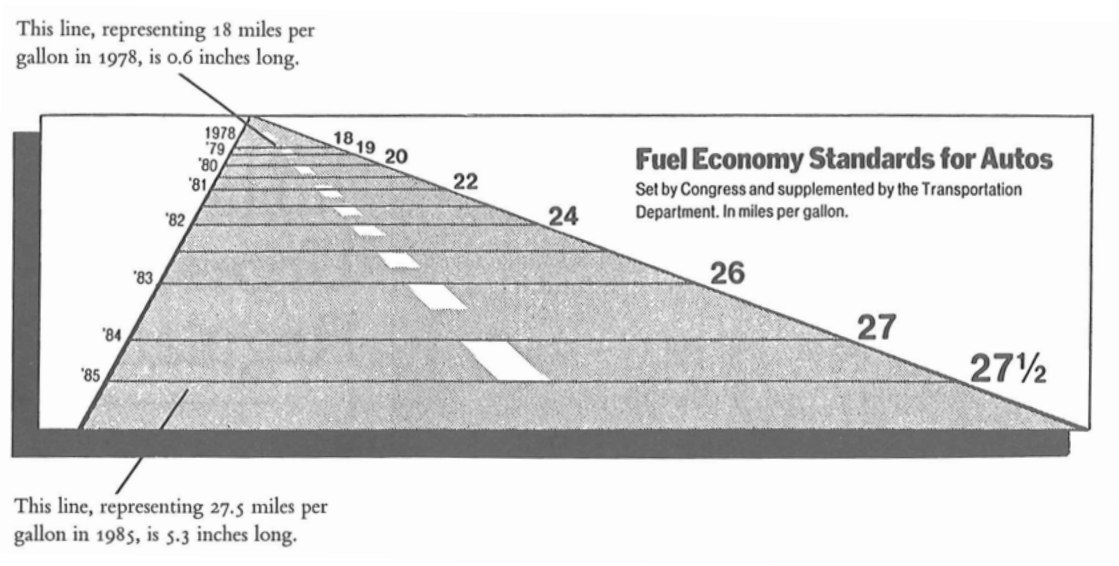
\includegraphics[keepaspectratio]{road.png}}

{[}Tufte, 1991{]} Edward Tufte, The Visual Display of Quantitative
Information, Second Edition, Graphics Press, USA, 1991, p.~57 -- 69.

\[\operatorname{LieFactor} = \frac{\text{size of the effect visible on the chart}}{\text{size of the effect resulting from the data}}\]

\[\text{effect size} = \frac{|\text{second value}-\text{first value}|}{\text{first value}}\]

\pandocbounded{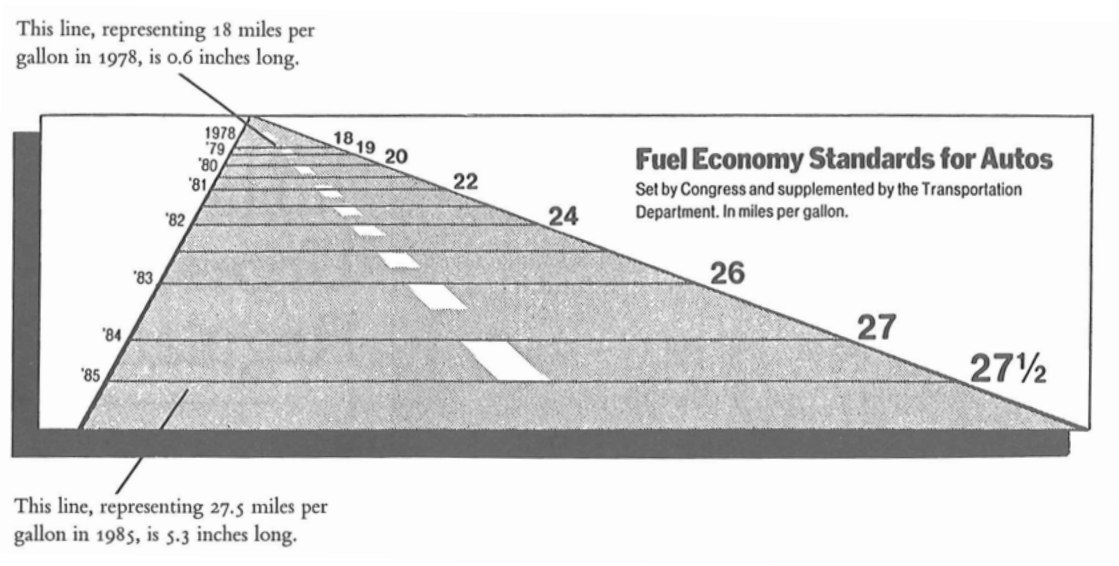
\includegraphics[keepaspectratio]{road.png}}

\[\operatorname{LieFactor} = \frac{\frac{5.3-0.6}{0.6}}{\frac{27.5-18}{18}} \approx 14.8\]

\section{References}\label{references-1}

\begin{itemize}
\tightlist
\item
  https://pl.wikipedia.org/wiki/Wizualizacja
\item
  https://mfiles.pl/pl/index.php/Analiza\_danych, accessed online
  1.04.2019.
\item
  Walesiak M., Gatnar E., Statystyczna analiza danych z wykorzystaniem
  programu R, PWN, Warszawa, 2009.
\item
  Wasilewska E., Statystyka opisowa od podstaw, Podręcznik z zadaniami,
  Wydawnictwo SGGW, Warszawa, 2009.
\item
  https://en.wikipedia.org/wiki/Cognitive\_reflection\_test, accessed
  online 20.03.2023.
\item
  https://qlikblog.pl/edward-tufte-dobre-praktyki-prezentacji-danych/,
  accessed online 20.03.2023.
\end{itemize}

\chapter{Configuration}\label{configuration}

\begin{enumerate}
\def\labelenumi{\arabic{enumi}.}
\tightlist
\item
  In the first step, we create a new project in the chosen location. We
  select venv and one of the Python versions, e.g.~3.13. Finally, click
  the Create button.
\end{enumerate}

\pandocbounded{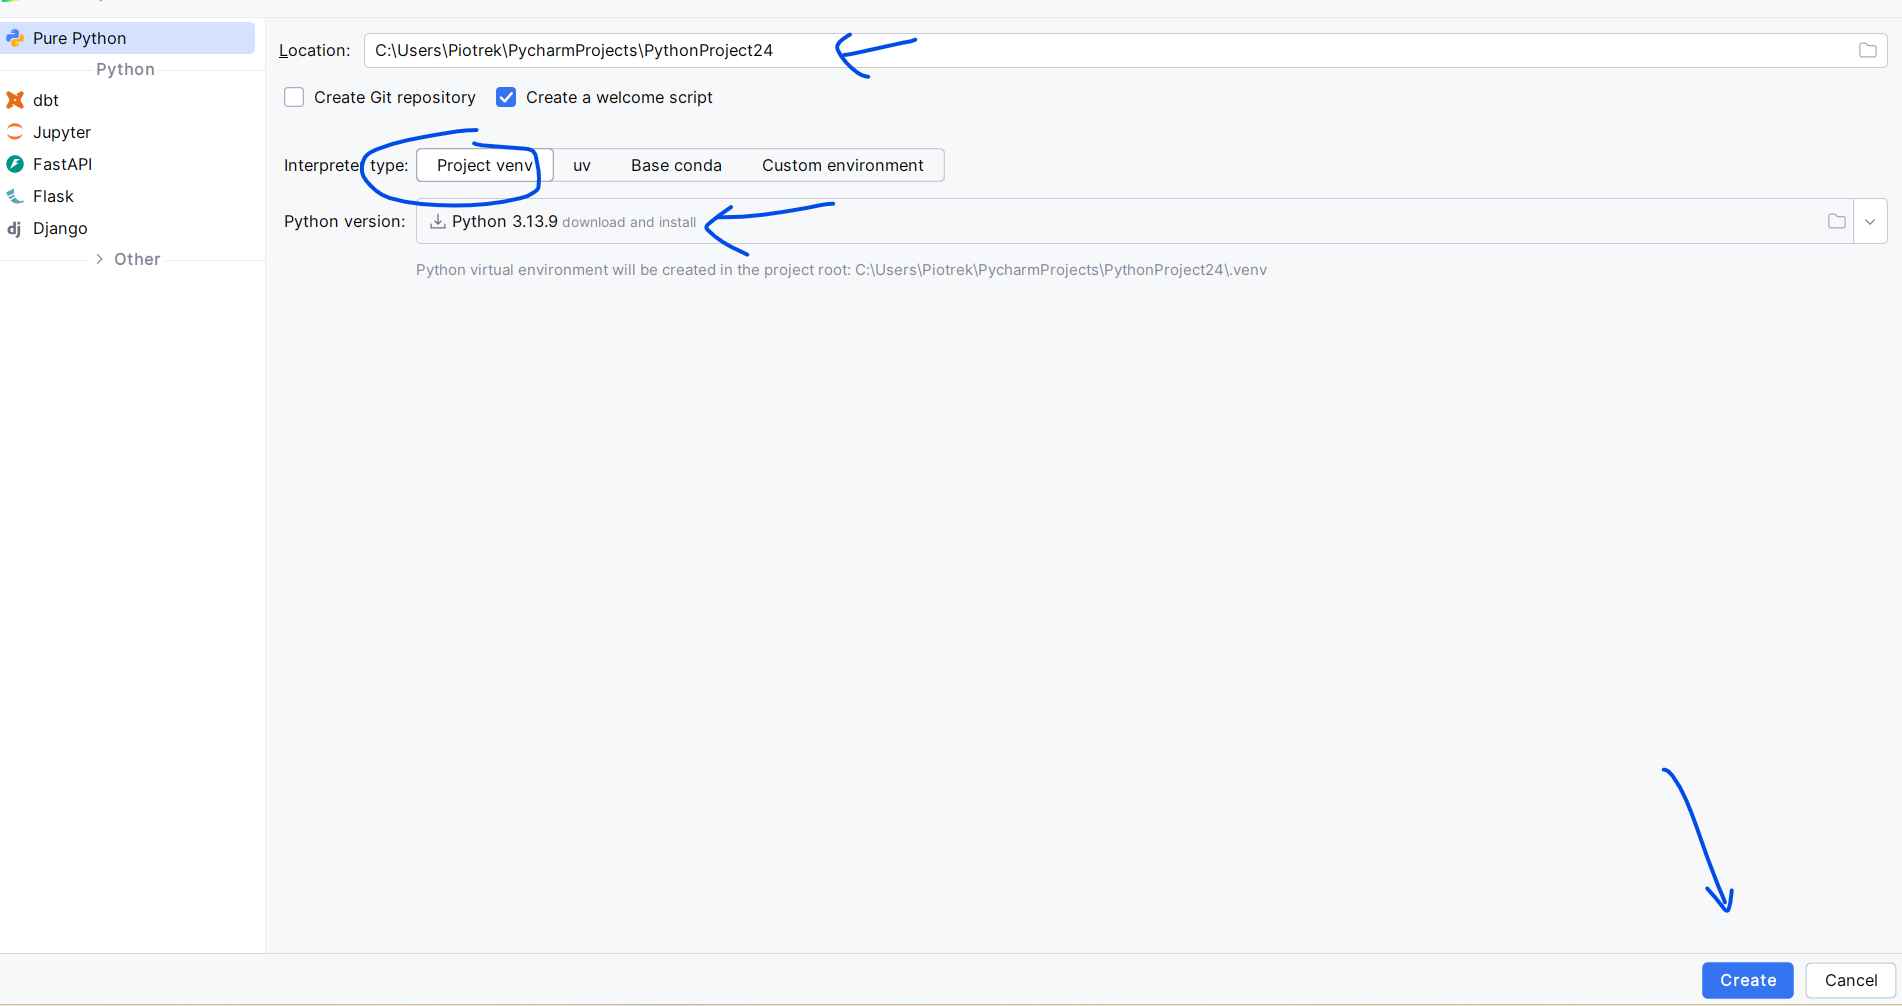
\includegraphics[keepaspectratio]{konf1.png}}

\begin{enumerate}
\def\labelenumi{\arabic{enumi}.}
\setcounter{enumi}{1}
\tightlist
\item
  We add the requirements file
  https://piojas.pl/wp-content/uploads/2026/02/requirements.txt to the
  project's root directory. The file name is important.
\end{enumerate}

\pandocbounded{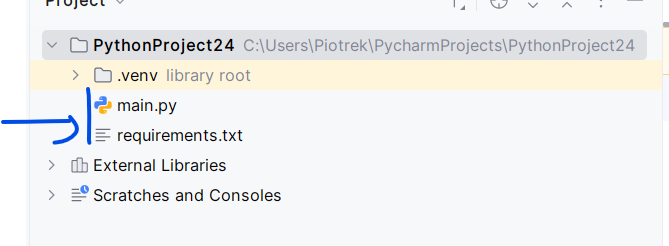
\includegraphics[keepaspectratio]{konf2.png}}

\begin{enumerate}
\def\labelenumi{\arabic{enumi}.}
\setcounter{enumi}{2}
\tightlist
\item
  We open the terminal in PyCharm and type the command:
  \texttt{pip\ install\ -r\ requirements.txt}
\end{enumerate}

\pandocbounded{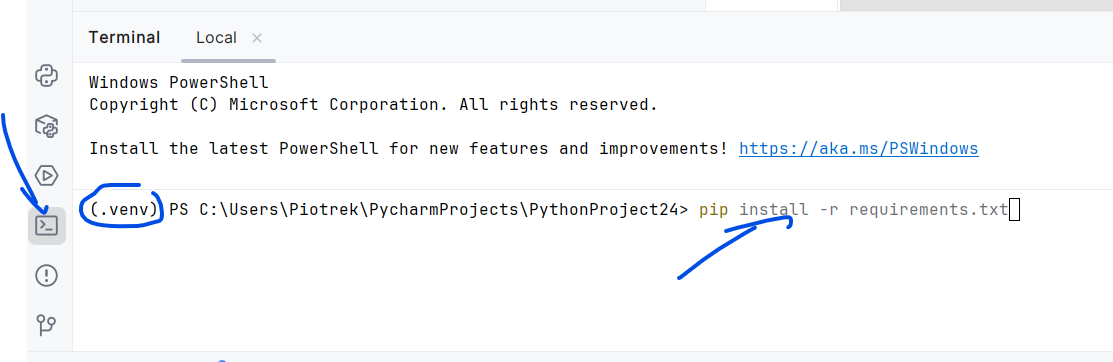
\includegraphics[keepaspectratio]{konf3.png}}

\part{NumPy}

\chapter{NumPy - Getting Started}\label{numpy---getting-started}

NumPy is a Python library for scientific computing.

Applications:

\begin{itemize}
\tightlist
\item
  linear algebra
\item
  advanced mathematical (numerical) computations
\item
  numerical integration
\item
  solving equations
\end{itemize}

\section{Importing the NumPy library}\label{importing-the-numpy-library}

\begin{Shaded}
\begin{Highlighting}[]
\ImportTok{import}\NormalTok{ numpy }\ImportTok{as}\NormalTok{ np}
\end{Highlighting}
\end{Shaded}

The fundamental object in the NumPy library is an N-dimensional array
called \texttt{ndarray}. Each element of the array is treated as a
\texttt{dtype} type.

\begin{Shaded}
\begin{Highlighting}[]
\NormalTok{np.array(}\BuiltInTok{object}\NormalTok{, dtype}\OperatorTok{=}\VariableTok{None}\NormalTok{, }\OperatorTok{*}\NormalTok{, copy}\OperatorTok{=}\VariableTok{True}\NormalTok{, order}\OperatorTok{=}\StringTok{\textquotesingle{}K\textquotesingle{}}\NormalTok{, subok}\OperatorTok{=}\VariableTok{False}\NormalTok{, ndmin}\OperatorTok{=}\DecValTok{0}\NormalTok{, like}\OperatorTok{=}\VariableTok{None}\NormalTok{)}
\end{Highlighting}
\end{Shaded}

\begin{itemize}
\tightlist
\item
  object - an object (or sequence) to be converted into an array
\item
  dtype - type
\item
  copy - whether objects should be copied, default is \texttt{True}
\item
  order - memory layout: C (rows), F (columns), A, K
\item
  subok - handled by subclasses (if \texttt{True}), default is
  \texttt{False}
\item
  ndmin - minimum number of dimensions of the array
\item
  like - creation based on a reference array
\end{itemize}

\protect\phantomsection\label{annotated-cell-3}%
\begin{Shaded}
\begin{Highlighting}[]
\ImportTok{import}\NormalTok{ numpy }\ImportTok{as}\NormalTok{ np}

\NormalTok{a }\OperatorTok{=}\NormalTok{ np.array([}\DecValTok{1}\NormalTok{, }\DecValTok{2}\NormalTok{, }\DecValTok{3}\NormalTok{]) }\hspace*{\fill}\NormalTok{\circled{1}}
\BuiltInTok{print}\NormalTok{(}\StringTok{"a:"}\NormalTok{, a) }
\BuiltInTok{print}\NormalTok{(}\StringTok{"type of a:"}\NormalTok{, }\BuiltInTok{type}\NormalTok{(a)) }\hspace*{\fill}\NormalTok{\circled{2}}
\NormalTok{b }\OperatorTok{=}\NormalTok{ np.array([}\DecValTok{1}\NormalTok{, }\DecValTok{2}\NormalTok{, }\FloatTok{3.0}\NormalTok{]) }\hspace*{\fill}\NormalTok{\circled{3}}
\BuiltInTok{print}\NormalTok{(}\StringTok{"b:"}\NormalTok{, b)}
\NormalTok{c }\OperatorTok{=}\NormalTok{ np.array([[}\DecValTok{1}\NormalTok{, }\DecValTok{2}\NormalTok{], [}\DecValTok{3}\NormalTok{, }\DecValTok{4}\NormalTok{]]) }\hspace*{\fill}\NormalTok{\circled{4}}
\BuiltInTok{print}\NormalTok{(}\StringTok{"c:"}\NormalTok{, c)}
\NormalTok{d }\OperatorTok{=}\NormalTok{ np.array([}\DecValTok{1}\NormalTok{, }\DecValTok{2}\NormalTok{, }\DecValTok{3}\NormalTok{], ndmin}\OperatorTok{=}\DecValTok{2}\NormalTok{) }\hspace*{\fill}\NormalTok{\circled{5}}
\BuiltInTok{print}\NormalTok{(}\StringTok{"d:"}\NormalTok{, d)}
\NormalTok{e }\OperatorTok{=}\NormalTok{ np.array([}\DecValTok{1}\NormalTok{, }\DecValTok{2}\NormalTok{, }\DecValTok{3}\NormalTok{], dtype}\OperatorTok{=}\BuiltInTok{complex}\NormalTok{) }\hspace*{\fill}\NormalTok{\circled{6}}
\BuiltInTok{print}\NormalTok{(}\StringTok{"e:"}\NormalTok{, e)}
\NormalTok{f }\OperatorTok{=}\NormalTok{ np.array(np.asmatrix(}\StringTok{\textquotesingle{}1 2; 3 4\textquotesingle{}}\NormalTok{)) }\hspace*{\fill}\NormalTok{\circled{7}}
\BuiltInTok{print}\NormalTok{(}\StringTok{"f:"}\NormalTok{, f)}
\NormalTok{g }\OperatorTok{=}\NormalTok{ np.array(np.asmatrix(}\StringTok{\textquotesingle{}1 2; 3 4\textquotesingle{}}\NormalTok{), subok}\OperatorTok{=}\VariableTok{True}\NormalTok{) }\hspace*{\fill}\NormalTok{\circled{8}}
\BuiltInTok{print}\NormalTok{(}\StringTok{"g:"}\NormalTok{, g)}
\BuiltInTok{print}\NormalTok{(}\BuiltInTok{type}\NormalTok{(g))}
\end{Highlighting}
\end{Shaded}

\begin{description}
\tightlist
\item[\circled{1}]
Creating an array with default settings.
\item[\circled{2}]
Checking the type.
\item[\circled{3}]
One of the elements is of a different type. Therefore, upcasting to the
``largest'' type occurs.
\item[\circled{4}]
Here we get a 2x2 array.
\item[\circled{5}]
In this line we get an array with dimensions 1x3 (shape
\texttt{(1,\ 3)}).
\item[\circled{6}]
Forcing the \texttt{complex} type --- a type with a wider range.
\item[\circled{7}]
Using the matrix subtype.
\item[\circled{8}]
Preserving the matrix type.
\end{description}

\begin{verbatim}
a: [1 2 3]
type of a: <class 'numpy.ndarray'>
b: [1. 2. 3.]
c: [[1 2]
 [3 4]]
d: [[1 2 3]]
e: [1.+0.j 2.+0.j 3.+0.j]
f: [[1 2]
 [3 4]]
g: [[1 2]
 [3 4]]
<class 'numpy.matrix'>
\end{verbatim}

\chapter{List vs Array}\label{list-vs-array}

\begin{Shaded}
\begin{Highlighting}[]
\ImportTok{import}\NormalTok{ numpy }\ImportTok{as}\NormalTok{ np}
\ImportTok{import}\NormalTok{ time}

\NormalTok{start\_time }\OperatorTok{=}\NormalTok{ time.time()}
\NormalTok{my\_arr }\OperatorTok{=}\NormalTok{ np.arange(}\DecValTok{1000000}\NormalTok{)}
\NormalTok{my\_list }\OperatorTok{=} \BuiltInTok{list}\NormalTok{(}\BuiltInTok{range}\NormalTok{(}\DecValTok{1000000}\NormalTok{))}
\NormalTok{start\_time }\OperatorTok{=}\NormalTok{ time.time()}
\NormalTok{my\_arr2 }\OperatorTok{=}\NormalTok{ my\_arr }\OperatorTok{*} \DecValTok{2}
\BuiltInTok{print}\NormalTok{(}\StringTok{"{-}{-}{-} }\SpecialCharTok{\%s}\StringTok{ seconds {-}{-}{-}"} \OperatorTok{\%}\NormalTok{ (time.time() }\OperatorTok{{-}}\NormalTok{ start\_time))}
\NormalTok{start\_time }\OperatorTok{=}\NormalTok{ time.time()}
\NormalTok{my\_list2 }\OperatorTok{=}\NormalTok{ [x }\OperatorTok{*} \DecValTok{2} \ControlFlowTok{for}\NormalTok{ x }\KeywordTok{in}\NormalTok{ my\_list]}
\BuiltInTok{print}\NormalTok{(}\StringTok{"{-}{-}{-} }\SpecialCharTok{\%s}\StringTok{ seconds {-}{-}{-}"} \OperatorTok{\%}\NormalTok{ (time.time() }\OperatorTok{{-}}\NormalTok{ start\_time))}
\end{Highlighting}
\end{Shaded}

\begin{verbatim}
--- 0.0020012855529785156 seconds ---
--- 0.036900997161865234 seconds ---
\end{verbatim}

\chapter{Array Attributes}\label{array-attributes}

{\def\LTcaptype{none} % do not increment counter
\begin{longtable}[]{@{}
  >{\raggedright\arraybackslash}p{(\linewidth - 2\tabcolsep) * \real{0.5000}}
  >{\raggedright\arraybackslash}p{(\linewidth - 2\tabcolsep) * \real{0.5000}}@{}}
\toprule\noalign{}
\begin{minipage}[b]{\linewidth}\raggedright
Attribute
\end{minipage} & \begin{minipage}[b]{\linewidth}\raggedright
Description
\end{minipage} \\
\midrule\noalign{}
\endhead
\bottomrule\noalign{}
\endlastfoot
\texttt{shape} & tuple with information about the number of elements for
each dimension \\
\texttt{size} & total number of elements in the array \\
\texttt{ndim} & number of dimensions of the array \\
\texttt{nbytes} & number of bytes the array occupies in memory \\
\texttt{dtype} & data type stored in the array (e.g.~\texttt{int64},
\texttt{float64}) \\
\end{longtable}
}

\begin{Shaded}
\begin{Highlighting}[]
\ImportTok{import}\NormalTok{ numpy }\ImportTok{as}\NormalTok{ np}

\NormalTok{tab1 }\OperatorTok{=}\NormalTok{ np.array([}\DecValTok{2}\NormalTok{, }\OperatorTok{{-}}\DecValTok{3}\NormalTok{, }\DecValTok{4}\NormalTok{, }\OperatorTok{{-}}\DecValTok{8}\NormalTok{, }\DecValTok{1}\NormalTok{])}
\BuiltInTok{print}\NormalTok{(}\StringTok{"type:"}\NormalTok{, }\BuiltInTok{type}\NormalTok{(tab1))}
\BuiltInTok{print}\NormalTok{(}\StringTok{"shape:"}\NormalTok{, tab1.shape)}
\BuiltInTok{print}\NormalTok{(}\StringTok{"size:"}\NormalTok{, tab1.size)}
\BuiltInTok{print}\NormalTok{(}\StringTok{"ndim:"}\NormalTok{, tab1.ndim)}
\BuiltInTok{print}\NormalTok{(}\StringTok{"nbytes:"}\NormalTok{, tab1.nbytes)}
\BuiltInTok{print}\NormalTok{(}\StringTok{"dtype:"}\NormalTok{, tab1.dtype)}
\end{Highlighting}
\end{Shaded}

\begin{verbatim}
type: <class 'numpy.ndarray'>
shape: (5,)
size: 5
ndim: 1
nbytes: 40
dtype: int64
\end{verbatim}

\begin{Shaded}
\begin{Highlighting}[]
\ImportTok{import}\NormalTok{ numpy }\ImportTok{as}\NormalTok{ np}

\NormalTok{tab2 }\OperatorTok{=}\NormalTok{ np.array([[}\DecValTok{2}\NormalTok{, }\OperatorTok{{-}}\DecValTok{3}\NormalTok{], [}\DecValTok{4}\NormalTok{, }\OperatorTok{{-}}\DecValTok{8}\NormalTok{]])}
\BuiltInTok{print}\NormalTok{(}\StringTok{"type:"}\NormalTok{, }\BuiltInTok{type}\NormalTok{(tab2))}
\BuiltInTok{print}\NormalTok{(}\StringTok{"shape:"}\NormalTok{, tab2.shape)}
\BuiltInTok{print}\NormalTok{(}\StringTok{"size:"}\NormalTok{, tab2.size)}
\BuiltInTok{print}\NormalTok{(}\StringTok{"ndim:"}\NormalTok{, tab2.ndim)}
\BuiltInTok{print}\NormalTok{(}\StringTok{"nbytes:"}\NormalTok{, tab2.nbytes)}
\BuiltInTok{print}\NormalTok{(}\StringTok{"dtype:"}\NormalTok{, tab2.dtype)}
\end{Highlighting}
\end{Shaded}

\begin{verbatim}
type: <class 'numpy.ndarray'>
shape: (2, 2)
size: 4
ndim: 2
nbytes: 32
dtype: int64
\end{verbatim}

NumPy does not support ragged arrays. The following code will produce an
error:

\begin{Shaded}
\begin{Highlighting}[]
\ImportTok{import}\NormalTok{ numpy }\ImportTok{as}\NormalTok{ np}

\NormalTok{tab3 }\OperatorTok{=}\NormalTok{ np.array([[}\DecValTok{2}\NormalTok{, }\OperatorTok{{-}}\DecValTok{3}\NormalTok{], [}\DecValTok{4}\NormalTok{, }\OperatorTok{{-}}\DecValTok{8}\NormalTok{, }\DecValTok{5}\NormalTok{], [}\DecValTok{3}\NormalTok{]])}
\end{Highlighting}
\end{Shaded}

\chapter{Data Types}\label{data-types}

{\def\LTcaptype{none} % do not increment counter
\begin{longtable}[]{@{}
  >{\raggedright\arraybackslash}p{(\linewidth - 2\tabcolsep) * \real{0.5000}}
  >{\raggedright\arraybackslash}p{(\linewidth - 2\tabcolsep) * \real{0.5000}}@{}}
\toprule\noalign{}
\endhead
\bottomrule\noalign{}
\endlastfoot
Integer types &
\texttt{int},\texttt{int8},\texttt{int16},\texttt{int32},\texttt{int64} \\
Unsigned integer types &
\texttt{uint},\texttt{uint8},\texttt{uint16},\texttt{uint32},\texttt{uint64} \\
Boolean type & \texttt{bool} \\
Floating-point types & \texttt{float}, \texttt{float16},
\texttt{float32}, \texttt{float64}, \texttt{float128} \\
Complex floating-point types & \texttt{complex}, \texttt{complex64},
\texttt{complex128}, \texttt{complex256} \\
String & \texttt{str} \\
\end{longtable}
}

\begin{Shaded}
\begin{Highlighting}[]
\ImportTok{import}\NormalTok{ numpy }\ImportTok{as}\NormalTok{ np}

\NormalTok{tab }\OperatorTok{=}\NormalTok{ np.array([[}\DecValTok{2}\NormalTok{, }\OperatorTok{{-}}\DecValTok{3}\NormalTok{], [}\DecValTok{4}\NormalTok{, }\OperatorTok{{-}}\DecValTok{8}\NormalTok{]])}
\BuiltInTok{print}\NormalTok{(tab)}
\NormalTok{tab2 }\OperatorTok{=}\NormalTok{ np.array([[}\DecValTok{2}\NormalTok{, }\OperatorTok{{-}}\DecValTok{3}\NormalTok{], [}\DecValTok{4}\NormalTok{, }\OperatorTok{{-}}\DecValTok{8}\NormalTok{]], dtype}\OperatorTok{=}\BuiltInTok{int}\NormalTok{)}
\BuiltInTok{print}\NormalTok{(tab2)}
\NormalTok{tab3 }\OperatorTok{=}\NormalTok{ np.array([[}\DecValTok{2}\NormalTok{, }\OperatorTok{{-}}\DecValTok{3}\NormalTok{], [}\DecValTok{4}\NormalTok{, }\OperatorTok{{-}}\DecValTok{8}\NormalTok{]], dtype}\OperatorTok{=}\BuiltInTok{float}\NormalTok{)}
\BuiltInTok{print}\NormalTok{(tab3)}
\NormalTok{tab4 }\OperatorTok{=}\NormalTok{ np.array([[}\DecValTok{2}\NormalTok{, }\OperatorTok{{-}}\DecValTok{3}\NormalTok{], [}\DecValTok{4}\NormalTok{, }\OperatorTok{{-}}\DecValTok{8}\NormalTok{]], dtype}\OperatorTok{=}\BuiltInTok{complex}\NormalTok{)}
\BuiltInTok{print}\NormalTok{(tab4)}
\end{Highlighting}
\end{Shaded}

\begin{verbatim}
[[ 2 -3]
 [ 4 -8]]
[[ 2 -3]
 [ 4 -8]]
[[ 2. -3.]
 [ 4. -8.]]
[[ 2.+0.j -3.+0.j]
 [ 4.+0.j -8.+0.j]]
\end{verbatim}

\chapter{Creating Arrays}\label{creating-arrays}

\texttt{np.array} - arguments are cast to an array (anything iterable) -
it's worth checking the size/shape

\begin{Shaded}
\begin{Highlighting}[]
\ImportTok{import}\NormalTok{ numpy }\ImportTok{as}\NormalTok{ np}

\NormalTok{tab }\OperatorTok{=}\NormalTok{ np.array([}\DecValTok{2}\NormalTok{, }\OperatorTok{{-}}\DecValTok{3}\NormalTok{, }\DecValTok{4}\NormalTok{])}
\BuiltInTok{print}\NormalTok{(tab)}
\BuiltInTok{print}\NormalTok{(}\StringTok{"size:"}\NormalTok{, tab.size)}
\NormalTok{tab2 }\OperatorTok{=}\NormalTok{ np.array((}\DecValTok{4}\NormalTok{, }\OperatorTok{{-}}\DecValTok{3}\NormalTok{, }\DecValTok{3}\NormalTok{, }\DecValTok{2}\NormalTok{))}
\BuiltInTok{print}\NormalTok{(tab2)}
\BuiltInTok{print}\NormalTok{(}\StringTok{"size:"}\NormalTok{, tab2.size)}
\NormalTok{tab3 }\OperatorTok{=}\NormalTok{ np.array(\{}\DecValTok{3}\NormalTok{, }\DecValTok{3}\NormalTok{, }\DecValTok{2}\NormalTok{, }\DecValTok{5}\NormalTok{, }\DecValTok{2}\NormalTok{\})}
\BuiltInTok{print}\NormalTok{(tab3)}
\BuiltInTok{print}\NormalTok{(}\StringTok{"size:"}\NormalTok{, tab3.size)}
\NormalTok{tab4 }\OperatorTok{=}\NormalTok{ np.array(\{}\StringTok{"pl"}\NormalTok{: }\DecValTok{344}\NormalTok{, }\StringTok{"en"}\NormalTok{: }\DecValTok{22}\NormalTok{\})}
\BuiltInTok{print}\NormalTok{(tab4)}
\BuiltInTok{print}\NormalTok{(}\StringTok{"size:"}\NormalTok{, tab4.size)}
\end{Highlighting}
\end{Shaded}

\begin{verbatim}
[ 2 -3  4]
size: 3
[ 4 -3  3  2]
size: 4
{2, 3, 5}
size: 1
{'pl': 344, 'en': 22}
size: 1
\end{verbatim}

\texttt{np.zeros} - creates an array filled with zeros

\begin{Shaded}
\begin{Highlighting}[]
\ImportTok{import}\NormalTok{ numpy }\ImportTok{as}\NormalTok{ np}

\NormalTok{tab }\OperatorTok{=}\NormalTok{ np.zeros(}\DecValTok{4}\NormalTok{)}
\BuiltInTok{print}\NormalTok{(tab)}
\BuiltInTok{print}\NormalTok{(tab.shape)}
\NormalTok{tab2 }\OperatorTok{=}\NormalTok{ np.zeros([}\DecValTok{2}\NormalTok{, }\DecValTok{3}\NormalTok{])}
\BuiltInTok{print}\NormalTok{(tab2)}
\BuiltInTok{print}\NormalTok{(tab2.shape)}
\NormalTok{tab3 }\OperatorTok{=}\NormalTok{ np.zeros([}\DecValTok{2}\NormalTok{, }\DecValTok{3}\NormalTok{, }\DecValTok{4}\NormalTok{])}
\BuiltInTok{print}\NormalTok{(tab3)}
\BuiltInTok{print}\NormalTok{(tab3.shape)}
\end{Highlighting}
\end{Shaded}

\begin{verbatim}
[0. 0. 0. 0.]
(4,)
[[0. 0. 0.]
 [0. 0. 0.]]
(2, 3)
[[[0. 0. 0. 0.]
  [0. 0. 0. 0.]
  [0. 0. 0. 0.]]

 [[0. 0. 0. 0.]
  [0. 0. 0. 0.]
  [0. 0. 0. 0.]]]
(2, 3, 4)
\end{verbatim}

\texttt{np.ones} - creates an array filled with ones (this is not the
equivalent of an identity matrix!)

\begin{Shaded}
\begin{Highlighting}[]
\ImportTok{import}\NormalTok{ numpy }\ImportTok{as}\NormalTok{ np}

\NormalTok{tab }\OperatorTok{=}\NormalTok{ np.ones(}\DecValTok{4}\NormalTok{)}
\BuiltInTok{print}\NormalTok{(tab)}
\BuiltInTok{print}\NormalTok{(tab.shape)}
\NormalTok{tab2 }\OperatorTok{=}\NormalTok{ np.ones([}\DecValTok{2}\NormalTok{, }\DecValTok{3}\NormalTok{])}
\BuiltInTok{print}\NormalTok{(tab2)}
\BuiltInTok{print}\NormalTok{(tab2.shape)}
\NormalTok{tab3 }\OperatorTok{=}\NormalTok{ np.ones([}\DecValTok{2}\NormalTok{, }\DecValTok{3}\NormalTok{, }\DecValTok{4}\NormalTok{])}
\BuiltInTok{print}\NormalTok{(tab3)}
\BuiltInTok{print}\NormalTok{(tab3.shape)}
\end{Highlighting}
\end{Shaded}

\begin{verbatim}
[1. 1. 1. 1.]
(4,)
[[1. 1. 1.]
 [1. 1. 1.]]
(2, 3)
[[[1. 1. 1. 1.]
  [1. 1. 1. 1.]
  [1. 1. 1. 1.]]

 [[1. 1. 1. 1.]
  [1. 1. 1. 1.]
  [1. 1. 1. 1.]]]
(2, 3, 4)
\end{verbatim}

\texttt{np.diag} - creates an array corresponding to a diagonal matrix

\begin{Shaded}
\begin{Highlighting}[]
\ImportTok{import}\NormalTok{ numpy }\ImportTok{as}\NormalTok{ np}

\BuiltInTok{print}\NormalTok{(}\StringTok{"tab0"}\NormalTok{)}
\NormalTok{tab0 }\OperatorTok{=}\NormalTok{ np.diag([}\DecValTok{3}\NormalTok{, }\DecValTok{4}\NormalTok{, }\DecValTok{5}\NormalTok{])}
\BuiltInTok{print}\NormalTok{(tab0)}
\BuiltInTok{print}\NormalTok{(}\StringTok{"tab1"}\NormalTok{)}
\NormalTok{tab1 }\OperatorTok{=}\NormalTok{ np.array([[}\DecValTok{2}\NormalTok{, }\DecValTok{3}\NormalTok{, }\DecValTok{4}\NormalTok{], [}\DecValTok{3}\NormalTok{, }\OperatorTok{{-}}\DecValTok{4}\NormalTok{, }\DecValTok{5}\NormalTok{], [}\DecValTok{3}\NormalTok{, }\DecValTok{4}\NormalTok{, }\OperatorTok{{-}}\DecValTok{5}\NormalTok{]])}
\BuiltInTok{print}\NormalTok{(tab1)}
\NormalTok{tab2 }\OperatorTok{=}\NormalTok{ np.diag(tab1)}
\BuiltInTok{print}\NormalTok{(}\StringTok{"tab2"}\NormalTok{)}
\BuiltInTok{print}\NormalTok{(tab2)}
\NormalTok{tab3 }\OperatorTok{=}\NormalTok{ np.diag(tab1, k}\OperatorTok{=}\DecValTok{1}\NormalTok{)}
\BuiltInTok{print}\NormalTok{(}\StringTok{"tab3"}\NormalTok{)}
\BuiltInTok{print}\NormalTok{(tab3)}
\BuiltInTok{print}\NormalTok{(}\StringTok{"tab4"}\NormalTok{)}
\NormalTok{tab4 }\OperatorTok{=}\NormalTok{ np.diag(tab1, k}\OperatorTok{={-}}\DecValTok{2}\NormalTok{)}
\BuiltInTok{print}\NormalTok{(tab4)}
\BuiltInTok{print}\NormalTok{(}\StringTok{"tab5"}\NormalTok{)}
\NormalTok{tab5 }\OperatorTok{=}\NormalTok{ np.diag(np.diag(tab1))}
\BuiltInTok{print}\NormalTok{(tab5)}
\end{Highlighting}
\end{Shaded}

\begin{verbatim}
tab0
[[3 0 0]
 [0 4 0]
 [0 0 5]]
tab1
[[ 2  3  4]
 [ 3 -4  5]
 [ 3  4 -5]]
tab2
[ 2 -4 -5]
tab3
[3 5]
tab4
[3]
tab5
[[ 2  0  0]
 [ 0 -4  0]
 [ 0  0 -5]]
\end{verbatim}

\texttt{np.arange} - array filled with evenly spaced values

Syntax:
\texttt{numpy.arange({[}start,\ {]}stop,\ {[}step,\ {]}dtype=None)}

Works similarly to the \texttt{range} function, but allows fractional
numbers.

\begin{Shaded}
\begin{Highlighting}[]
\ImportTok{import}\NormalTok{ numpy }\ImportTok{as}\NormalTok{ np}

\NormalTok{a }\OperatorTok{=}\NormalTok{ np.arange(}\DecValTok{3}\NormalTok{)}
\BuiltInTok{print}\NormalTok{(a)}
\NormalTok{b }\OperatorTok{=}\NormalTok{ np.arange(}\FloatTok{3.0}\NormalTok{)}
\BuiltInTok{print}\NormalTok{(b)}
\NormalTok{c }\OperatorTok{=}\NormalTok{ np.arange(}\DecValTok{3}\NormalTok{, }\DecValTok{7}\NormalTok{)}
\BuiltInTok{print}\NormalTok{(c)}
\NormalTok{d }\OperatorTok{=}\NormalTok{ np.arange(}\DecValTok{3}\NormalTok{, }\DecValTok{11}\NormalTok{, }\DecValTok{2}\NormalTok{)}
\BuiltInTok{print}\NormalTok{(d)}
\NormalTok{e }\OperatorTok{=}\NormalTok{ np.arange(}\DecValTok{0}\NormalTok{, }\DecValTok{1}\NormalTok{, }\FloatTok{0.1}\NormalTok{)}
\BuiltInTok{print}\NormalTok{(e)}
\NormalTok{f }\OperatorTok{=}\NormalTok{ np.arange(}\DecValTok{3}\NormalTok{, }\DecValTok{11}\NormalTok{, }\DecValTok{2}\NormalTok{, dtype}\OperatorTok{=}\BuiltInTok{float}\NormalTok{)}
\BuiltInTok{print}\NormalTok{(f)}
\NormalTok{g }\OperatorTok{=}\NormalTok{ np.arange(}\DecValTok{3}\NormalTok{, }\DecValTok{10}\NormalTok{, }\DecValTok{2}\NormalTok{)}
\BuiltInTok{print}\NormalTok{(g)}
\end{Highlighting}
\end{Shaded}

\begin{verbatim}
[0 1 2]
[0. 1. 2.]
[3 4 5 6]
[3 5 7 9]
[0.  0.1 0.2 0.3 0.4 0.5 0.6 0.7 0.8 0.9]
[3. 5. 7. 9.]
[3 5 7 9]
\end{verbatim}

\texttt{np.linspace} - array filled with evenly spaced values on a
linear scale

\texttt{np.linspace(start,\ stop,\ num)} generates an array of evenly
spaced values. For example, \texttt{np.linspace(2.0,\ 3.0,\ num=5)}
produces \texttt{2,\ 2.25,\ 2.5,\ 2.75,\ 3} --- the interval is divided
into \texttt{num\ -\ 1} equal parts. Setting \texttt{endpoint=False}
removes the last point (from the right side), and the interval is then
divided into \texttt{num} equal parts instead. The \texttt{dtype}
parameter forces the output type --- typically set to \texttt{int}, in
which case the results may have the fractional part truncated.

\begin{Shaded}
\begin{Highlighting}[]
\ImportTok{import}\NormalTok{ numpy }\ImportTok{as}\NormalTok{ np}

\NormalTok{a }\OperatorTok{=}\NormalTok{ np.linspace(}\FloatTok{2.0}\NormalTok{, }\FloatTok{3.0}\NormalTok{, num}\OperatorTok{=}\DecValTok{5}\NormalTok{)}
\BuiltInTok{print}\NormalTok{(a)}
\NormalTok{b }\OperatorTok{=}\NormalTok{ np.linspace(}\FloatTok{2.0}\NormalTok{, }\FloatTok{3.0}\NormalTok{, num}\OperatorTok{=}\DecValTok{5}\NormalTok{, endpoint}\OperatorTok{=}\VariableTok{False}\NormalTok{)}
\BuiltInTok{print}\NormalTok{(b)}
\NormalTok{c }\OperatorTok{=}\NormalTok{ np.linspace(}\DecValTok{10}\NormalTok{, }\DecValTok{20}\NormalTok{, num}\OperatorTok{=}\DecValTok{4}\NormalTok{)}
\BuiltInTok{print}\NormalTok{(c)}
\NormalTok{d }\OperatorTok{=}\NormalTok{ np.linspace(}\DecValTok{10}\NormalTok{, }\DecValTok{20}\NormalTok{, num}\OperatorTok{=}\DecValTok{4}\NormalTok{, dtype}\OperatorTok{=}\BuiltInTok{int}\NormalTok{)}
\BuiltInTok{print}\NormalTok{(d)}
\end{Highlighting}
\end{Shaded}

\begin{verbatim}
[2.   2.25 2.5  2.75 3.  ]
[2.  2.2 2.4 2.6 2.8]
[10.         13.33333333 16.66666667 20.        ]
[10 13 16 20]
\end{verbatim}

\texttt{np.logspace} - array filled with values on a logarithmic scale

Syntax:
\texttt{numpy.logspace(start,\ stop,\ num=50,\ endpoint=True,\ base=10.0,\ dtype=None,\ axis=0)}

The function \texttt{np.logspace(2.0,\ 3.0,\ num=4)} generates 4 numbers
spaced evenly on a logarithmic scale between 10\^{}2 and 10\^{}3. The
default base is 10. First, the exponents are computed as equally spaced
points in the interval {[}2.0, 3.0{]}, which gives approximately 2,
2.33, 2.66, and 3.0. Then each exponent is used as the power of 10,
producing the output values 10\^{}2 = 100, 10\^{}2.33 ≈ 215.44,
10\^{}2.66 ≈ 464.16, and 10\^{}3 = 1000. An important consequence is
that while the exponents are uniformly distributed, the resulting values
are not --- the distances between consecutive output numbers grow larger
as the values increase. This is the key distinction between
\texttt{np.logspace} and \texttt{np.linspace}: the former creates equal
spacing in log-scale (i.e.~between the exponents), not in the actual
output values.

\begin{Shaded}
\begin{Highlighting}[]
\ImportTok{import}\NormalTok{ numpy }\ImportTok{as}\NormalTok{ np}

\NormalTok{a }\OperatorTok{=}\NormalTok{ np.logspace(}\FloatTok{2.0}\NormalTok{, }\FloatTok{3.0}\NormalTok{, num}\OperatorTok{=}\DecValTok{4}\NormalTok{)}
\BuiltInTok{print}\NormalTok{(a)}
\NormalTok{b }\OperatorTok{=}\NormalTok{ np.logspace(}\FloatTok{2.0}\NormalTok{, }\FloatTok{3.0}\NormalTok{, num}\OperatorTok{=}\DecValTok{4}\NormalTok{, endpoint}\OperatorTok{=}\VariableTok{False}\NormalTok{)}
\BuiltInTok{print}\NormalTok{(b)}
\NormalTok{c }\OperatorTok{=}\NormalTok{ np.logspace(}\FloatTok{2.0}\NormalTok{, }\FloatTok{3.0}\NormalTok{, num}\OperatorTok{=}\DecValTok{4}\NormalTok{, base}\OperatorTok{=}\FloatTok{2.0}\NormalTok{)}
\BuiltInTok{print}\NormalTok{(c)}
\end{Highlighting}
\end{Shaded}

\begin{verbatim}
[ 100.          215.443469    464.15888336 1000.        ]
[100.         177.827941   316.22776602 562.34132519]
[4.         5.0396842  6.34960421 8.        ]
\end{verbatim}

\texttt{np.empty} - empty (uninitialized) array - specific values are
not ``guaranteed''

\begin{Shaded}
\begin{Highlighting}[]
\ImportTok{import}\NormalTok{ numpy }\ImportTok{as}\NormalTok{ np}

\NormalTok{a }\OperatorTok{=}\NormalTok{ np.empty(}\DecValTok{3}\NormalTok{)}
\BuiltInTok{print}\NormalTok{(a)}
\NormalTok{b }\OperatorTok{=}\NormalTok{ np.empty(}\DecValTok{3}\NormalTok{, dtype}\OperatorTok{=}\BuiltInTok{int}\NormalTok{)}
\BuiltInTok{print}\NormalTok{(b)}
\end{Highlighting}
\end{Shaded}

\begin{verbatim}
[0. 1. 2.]
[                  0 4607182418800017408 4611686018427387904]
\end{verbatim}

\texttt{np.identity} - array resembling an identity matrix

\texttt{np.eye} - array with ones on the diagonal (remaining values are
zeros)

\begin{Shaded}
\begin{Highlighting}[]
\ImportTok{import}\NormalTok{ numpy }\ImportTok{as}\NormalTok{ np}

\BuiltInTok{print}\NormalTok{(}\StringTok{"a"}\NormalTok{)}
\NormalTok{a }\OperatorTok{=}\NormalTok{ np.identity(}\DecValTok{4}\NormalTok{)}
\BuiltInTok{print}\NormalTok{(a)}
\BuiltInTok{print}\NormalTok{(}\StringTok{"b"}\NormalTok{)}
\NormalTok{b }\OperatorTok{=}\NormalTok{ np.eye(}\DecValTok{4}\NormalTok{, k}\OperatorTok{=}\DecValTok{1}\NormalTok{)}
\BuiltInTok{print}\NormalTok{(b)}
\BuiltInTok{print}\NormalTok{(}\StringTok{"c"}\NormalTok{)}
\NormalTok{c }\OperatorTok{=}\NormalTok{ np.eye(}\DecValTok{4}\NormalTok{, k}\OperatorTok{=}\DecValTok{2}\NormalTok{)}
\BuiltInTok{print}\NormalTok{(c)}
\BuiltInTok{print}\NormalTok{(}\StringTok{"d"}\NormalTok{)}
\NormalTok{d }\OperatorTok{=}\NormalTok{ np.eye(}\DecValTok{4}\NormalTok{, k}\OperatorTok{={-}}\DecValTok{1}\NormalTok{)}
\BuiltInTok{print}\NormalTok{(d)}
\end{Highlighting}
\end{Shaded}

\begin{verbatim}
a
[[1. 0. 0. 0.]
 [0. 1. 0. 0.]
 [0. 0. 1. 0.]
 [0. 0. 0. 1.]]
b
[[0. 1. 0. 0.]
 [0. 0. 1. 0.]
 [0. 0. 0. 1.]
 [0. 0. 0. 0.]]
c
[[0. 0. 1. 0.]
 [0. 0. 0. 1.]
 [0. 0. 0. 0.]
 [0. 0. 0. 0.]]
d
[[0. 0. 0. 0.]
 [1. 0. 0. 0.]
 [0. 1. 0. 0.]
 [0. 0. 1. 0.]]
\end{verbatim}

\chapter{Indexing, ``slicing''}\label{indexing-slicing}

\protect\phantomsection\label{annotated-cell-18}%
\begin{Shaded}
\begin{Highlighting}[]
\ImportTok{import}\NormalTok{ numpy }\ImportTok{as}\NormalTok{ np}

\NormalTok{a }\OperatorTok{=}\NormalTok{ np.array([}\DecValTok{2}\NormalTok{, }\DecValTok{5}\NormalTok{, }\OperatorTok{{-}}\DecValTok{2}\NormalTok{, }\DecValTok{4}\NormalTok{, }\OperatorTok{{-}}\DecValTok{7}\NormalTok{, }\DecValTok{8}\NormalTok{, }\DecValTok{9}\NormalTok{, }\DecValTok{11}\NormalTok{, }\OperatorTok{{-}}\DecValTok{23}\NormalTok{, }\OperatorTok{{-}}\DecValTok{4}\NormalTok{, }\OperatorTok{{-}}\DecValTok{7}\NormalTok{, }\DecValTok{16}\NormalTok{, }\DecValTok{1}\NormalTok{])}
\BuiltInTok{print}\NormalTok{(}\StringTok{"1:"}\NormalTok{, a[}\DecValTok{5}\NormalTok{]) }\hspace*{\fill}\NormalTok{\circled{1}}
\BuiltInTok{print}\NormalTok{(}\StringTok{"2:"}\NormalTok{, a[}\OperatorTok{{-}}\DecValTok{2}\NormalTok{]) }\hspace*{\fill}\NormalTok{\circled{2}}
\BuiltInTok{print}\NormalTok{(}\StringTok{"3:"}\NormalTok{, a[}\DecValTok{3}\NormalTok{:}\DecValTok{6}\NormalTok{]) }\hspace*{\fill}\NormalTok{\circled{3}}
\BuiltInTok{print}\NormalTok{(}\StringTok{"4:"}\NormalTok{, a[:]) }\hspace*{\fill}\NormalTok{\circled{4}}
\BuiltInTok{print}\NormalTok{(}\StringTok{"5:"}\NormalTok{, a[}\DecValTok{0}\NormalTok{:}\OperatorTok{{-}}\DecValTok{1}\NormalTok{]) }\hspace*{\fill}\NormalTok{\circled{5}}
\BuiltInTok{print}\NormalTok{(}\StringTok{"6:"}\NormalTok{, a[:}\DecValTok{5}\NormalTok{]) }\hspace*{\fill}\NormalTok{\circled{6}}
\end{Highlighting}
\end{Shaded}

\begin{description}
\tightlist
\item[\circled{1}]
Access the element at index 5.
\item[\circled{2}]
Access the second element from the end.
\item[\circled{3}]
Access elements with indices from 3 to 5 (inclusive) --- the principle
of half-open intervals (closed on the left, open on the right).
\item[\circled{4}]
Access all elements.
\item[\circled{5}]
Access all elements except the last one.
\item[\circled{6}]
Access from the beginning up to the element at index 4.
\end{description}

\begin{verbatim}
1: 8
2: 16
3: [ 4 -7  8]
4: [  2   5  -2   4  -7   8   9  11 -23  -4  -7  16   1]
5: [  2   5  -2   4  -7   8   9  11 -23  -4  -7  16]
6: [ 2  5 -2  4 -7]
\end{verbatim}

\protect\phantomsection\label{annotated-cell-19}%
\begin{Shaded}
\begin{Highlighting}[]
\ImportTok{import}\NormalTok{ numpy }\ImportTok{as}\NormalTok{ np}

\BuiltInTok{print}\NormalTok{(}\StringTok{"1:"}\NormalTok{, a[}\DecValTok{4}\NormalTok{:]) }\hspace*{\fill}\NormalTok{\circled{1}}
\BuiltInTok{print}\NormalTok{(}\StringTok{"2:"}\NormalTok{, a[}\DecValTok{4}\NormalTok{:}\OperatorTok{{-}}\DecValTok{1}\NormalTok{]) }\hspace*{\fill}\NormalTok{\circled{2}}
\BuiltInTok{print}\NormalTok{(}\StringTok{"3:"}\NormalTok{, a[}\DecValTok{4}\NormalTok{:}\DecValTok{10}\NormalTok{:}\DecValTok{2}\NormalTok{]) }\hspace*{\fill}\NormalTok{\circled{3}}
\BuiltInTok{print}\NormalTok{(}\StringTok{"4:"}\NormalTok{, a[::}\OperatorTok{{-}}\DecValTok{1}\NormalTok{]) }\hspace*{\fill}\NormalTok{\circled{4}}
\BuiltInTok{print}\NormalTok{(}\StringTok{"5:"}\NormalTok{, a[::}\DecValTok{2}\NormalTok{]) }\hspace*{\fill}\NormalTok{\circled{5}}
\BuiltInTok{print}\NormalTok{(}\StringTok{"6:"}\NormalTok{, a[::}\OperatorTok{{-}}\DecValTok{2}\NormalTok{]) }\hspace*{\fill}\NormalTok{\circled{6}}
\end{Highlighting}
\end{Shaded}

\begin{description}
\tightlist
\item[\circled{1}]
Access elements from index 4 to the end.
\item[\circled{2}]
Access elements from index 4 to the end, excluding the last one.
\item[\circled{3}]
Access elements whose indices form an arithmetic sequence from 4 to 10
(including 4, but excluding 10) with a step of 2.
\item[\circled{4}]
Access elements in reverse order (from end to beginning).
\item[\circled{5}]
Access elements at even indices from the beginning.
\item[\circled{6}]
Access every second element, counting from the end (reversed order).
\end{description}

\begin{verbatim}
1: [ -7   8   9  11 -23  -4  -7  16   1]
2: [ -7   8   9  11 -23  -4  -7  16]
3: [ -7   9 -23]
4: [  1  16  -7  -4 -23  11   9   8  -7   4  -2   5   2]
5: [  2  -2  -7   9 -23  -7   1]
6: [  1  -7 -23   9  -7  -2   2]
\end{verbatim}

\begin{Shaded}
\begin{Highlighting}[]
\ImportTok{import}\NormalTok{ numpy }\ImportTok{as}\NormalTok{ np}

\NormalTok{a }\OperatorTok{=}\NormalTok{ np.array([[}\DecValTok{3}\NormalTok{, }\DecValTok{4}\NormalTok{, }\DecValTok{5}\NormalTok{], [}\OperatorTok{{-}}\DecValTok{3}\NormalTok{, }\DecValTok{4}\NormalTok{, }\DecValTok{8}\NormalTok{], [}\DecValTok{3}\NormalTok{, }\DecValTok{2}\NormalTok{, }\DecValTok{9}\NormalTok{]])}
\NormalTok{b }\OperatorTok{=}\NormalTok{ a[:}\DecValTok{2}\NormalTok{, }\DecValTok{1}\NormalTok{:]}
\BuiltInTok{print}\NormalTok{(b)}
\BuiltInTok{print}\NormalTok{(np.shape(b))}
\NormalTok{c }\OperatorTok{=}\NormalTok{ a[}\DecValTok{1}\NormalTok{]}
\BuiltInTok{print}\NormalTok{(c)}
\BuiltInTok{print}\NormalTok{(np.shape(c))}
\NormalTok{d }\OperatorTok{=}\NormalTok{ a[}\DecValTok{1}\NormalTok{, :]}
\BuiltInTok{print}\NormalTok{(d)}
\BuiltInTok{print}\NormalTok{(np.shape(d))}
\end{Highlighting}
\end{Shaded}

\begin{verbatim}
[[4 5]
 [4 8]]
(2, 2)
[-3  4  8]
(3,)
[-3  4  8]
(3,)
\end{verbatim}

\begin{Shaded}
\begin{Highlighting}[]
\ImportTok{import}\NormalTok{ numpy }\ImportTok{as}\NormalTok{ np}

\NormalTok{a }\OperatorTok{=}\NormalTok{ np.array([[}\DecValTok{3}\NormalTok{, }\DecValTok{4}\NormalTok{, }\DecValTok{5}\NormalTok{], [}\OperatorTok{{-}}\DecValTok{3}\NormalTok{, }\DecValTok{4}\NormalTok{, }\DecValTok{8}\NormalTok{], [}\DecValTok{3}\NormalTok{, }\DecValTok{2}\NormalTok{, }\DecValTok{9}\NormalTok{]])}
\NormalTok{e }\OperatorTok{=}\NormalTok{ a[}\DecValTok{1}\NormalTok{:}\DecValTok{2}\NormalTok{, :]}
\BuiltInTok{print}\NormalTok{(e)}
\BuiltInTok{print}\NormalTok{(np.shape(e))}
\NormalTok{f }\OperatorTok{=}\NormalTok{ a[:, :}\DecValTok{2}\NormalTok{]}
\BuiltInTok{print}\NormalTok{(f)}
\BuiltInTok{print}\NormalTok{(np.shape(f))}
\NormalTok{g }\OperatorTok{=}\NormalTok{ a[}\DecValTok{1}\NormalTok{, :}\DecValTok{2}\NormalTok{]}
\BuiltInTok{print}\NormalTok{(g)}
\BuiltInTok{print}\NormalTok{(np.shape(g))}
\NormalTok{h }\OperatorTok{=}\NormalTok{ a[}\DecValTok{1}\NormalTok{:}\DecValTok{2}\NormalTok{, :}\DecValTok{2}\NormalTok{]}
\BuiltInTok{print}\NormalTok{(h)}
\BuiltInTok{print}\NormalTok{(np.shape(h))}
\end{Highlighting}
\end{Shaded}

\begin{verbatim}
[[-3  4  8]]
(1, 3)
[[ 3  4]
 [-3  4]
 [ 3  2]]
(3, 2)
[-3  4]
(2,)
[[-3  4]]
(1, 2)
\end{verbatim}

\textbf{Note --- ``slicing'' creates a so-called view, not a copy.
Changes to the view affect the original array and vice versa.}

\begin{Shaded}
\begin{Highlighting}[]
\ImportTok{import}\NormalTok{ numpy }\ImportTok{as}\NormalTok{ np}

\NormalTok{a }\OperatorTok{=}\NormalTok{ np.array([[}\DecValTok{3}\NormalTok{, }\DecValTok{4}\NormalTok{, }\DecValTok{5}\NormalTok{], [}\OperatorTok{{-}}\DecValTok{3}\NormalTok{, }\DecValTok{4}\NormalTok{, }\DecValTok{8}\NormalTok{], [}\DecValTok{3}\NormalTok{, }\DecValTok{2}\NormalTok{, }\DecValTok{9}\NormalTok{]])}
\NormalTok{b }\OperatorTok{=}\NormalTok{ a[}\DecValTok{1}\NormalTok{:}\DecValTok{2}\NormalTok{, }\DecValTok{1}\NormalTok{:]}
\BuiltInTok{print}\NormalTok{(b)}
\NormalTok{a[}\DecValTok{1}\NormalTok{][}\DecValTok{1}\NormalTok{] }\OperatorTok{=} \DecValTok{9}
\BuiltInTok{print}\NormalTok{(a)}
\BuiltInTok{print}\NormalTok{(b)}
\NormalTok{b[}\DecValTok{0}\NormalTok{][}\DecValTok{0}\NormalTok{] }\OperatorTok{=} \OperatorTok{{-}}\DecValTok{11}
\BuiltInTok{print}\NormalTok{(a)}
\BuiltInTok{print}\NormalTok{(b)}
\end{Highlighting}
\end{Shaded}

\begin{verbatim}
[[4 8]]
[[ 3  4  5]
 [-3  9  8]
 [ 3  2  9]]
[[9 8]]
[[  3   4   5]
 [ -3 -11   8]
 [  3   2   9]]
[[-11   8]]
\end{verbatim}

Solution --- use the \texttt{.copy()} method:

\begin{Shaded}
\begin{Highlighting}[]
\ImportTok{import}\NormalTok{ numpy }\ImportTok{as}\NormalTok{ np}

\NormalTok{a }\OperatorTok{=}\NormalTok{ np.array([[}\DecValTok{3}\NormalTok{, }\DecValTok{4}\NormalTok{, }\DecValTok{5}\NormalTok{], [}\OperatorTok{{-}}\DecValTok{3}\NormalTok{, }\DecValTok{4}\NormalTok{, }\DecValTok{8}\NormalTok{], [}\DecValTok{3}\NormalTok{, }\DecValTok{2}\NormalTok{, }\DecValTok{9}\NormalTok{]])}
\NormalTok{b }\OperatorTok{=}\NormalTok{ a[}\DecValTok{1}\NormalTok{:}\DecValTok{2}\NormalTok{, }\DecValTok{1}\NormalTok{:].copy()}
\BuiltInTok{print}\NormalTok{(b)}
\NormalTok{a[}\DecValTok{1}\NormalTok{][}\DecValTok{1}\NormalTok{] }\OperatorTok{=} \DecValTok{9}
\BuiltInTok{print}\NormalTok{(a)}
\BuiltInTok{print}\NormalTok{(b)}
\NormalTok{b[}\DecValTok{0}\NormalTok{][}\DecValTok{0}\NormalTok{] }\OperatorTok{=} \OperatorTok{{-}}\DecValTok{11}
\BuiltInTok{print}\NormalTok{(a)}
\BuiltInTok{print}\NormalTok{(b)}
\end{Highlighting}
\end{Shaded}

\begin{verbatim}
[[4 8]]
[[ 3  4  5]
 [-3  9  8]
 [ 3  2  9]]
[[4 8]]
[[ 3  4  5]
 [-3  9  8]
 [ 3  2  9]]
[[-11   8]]
\end{verbatim}

Fancy indexing (indexing with an array of indices)

\begin{Shaded}
\begin{Highlighting}[]
\ImportTok{import}\NormalTok{ numpy }\ImportTok{as}\NormalTok{ np}

\NormalTok{a }\OperatorTok{=}\NormalTok{ np.array([}\DecValTok{2}\NormalTok{, }\DecValTok{5}\NormalTok{, }\OperatorTok{{-}}\DecValTok{2}\NormalTok{, }\DecValTok{4}\NormalTok{, }\OperatorTok{{-}}\DecValTok{7}\NormalTok{, }\DecValTok{8}\NormalTok{, }\DecValTok{9}\NormalTok{, }\DecValTok{11}\NormalTok{, }\OperatorTok{{-}}\DecValTok{23}\NormalTok{, }\OperatorTok{{-}}\DecValTok{4}\NormalTok{, }\OperatorTok{{-}}\DecValTok{7}\NormalTok{, }\DecValTok{8}\NormalTok{, }\DecValTok{1}\NormalTok{])}
\NormalTok{b }\OperatorTok{=}\NormalTok{ a[np.array([}\DecValTok{1}\NormalTok{, }\DecValTok{3}\NormalTok{, }\DecValTok{7}\NormalTok{])]}
\BuiltInTok{print}\NormalTok{(b)}
\NormalTok{c }\OperatorTok{=}\NormalTok{ a[[}\DecValTok{1}\NormalTok{, }\DecValTok{3}\NormalTok{, }\DecValTok{7}\NormalTok{]]}
\BuiltInTok{print}\NormalTok{(c)}
\end{Highlighting}
\end{Shaded}

\begin{verbatim}
[ 5  4 11]
[ 5  4 11]
\end{verbatim}

Boolean indexing (boolean masks)

\begin{Shaded}
\begin{Highlighting}[]
\ImportTok{import}\NormalTok{ numpy }\ImportTok{as}\NormalTok{ np}

\NormalTok{a }\OperatorTok{=}\NormalTok{ np.array([}\DecValTok{2}\NormalTok{, }\DecValTok{5}\NormalTok{, }\OperatorTok{{-}}\DecValTok{2}\NormalTok{, }\DecValTok{4}\NormalTok{, }\OperatorTok{{-}}\DecValTok{7}\NormalTok{, }\DecValTok{8}\NormalTok{, }\DecValTok{9}\NormalTok{, }\DecValTok{11}\NormalTok{, }\OperatorTok{{-}}\DecValTok{23}\NormalTok{, }\OperatorTok{{-}}\DecValTok{4}\NormalTok{, }\OperatorTok{{-}}\DecValTok{7}\NormalTok{, }\DecValTok{8}\NormalTok{, }\DecValTok{1}\NormalTok{])}
\NormalTok{b }\OperatorTok{=}\NormalTok{ a }\OperatorTok{\textgreater{}} \DecValTok{0}
\BuiltInTok{print}\NormalTok{(b)}
\NormalTok{c }\OperatorTok{=}\NormalTok{ a[a }\OperatorTok{\textgreater{}} \DecValTok{0}\NormalTok{]}
\BuiltInTok{print}\NormalTok{(c)}
\NormalTok{d }\OperatorTok{=}\NormalTok{ a[(a }\OperatorTok{\textgreater{}} \DecValTok{5}\NormalTok{) }\OperatorTok{\&}\NormalTok{ (a}\OperatorTok{\%}\DecValTok{2} \OperatorTok{!=}\DecValTok{0}\NormalTok{)] }\CommentTok{\# the \& operator stands for AND}
\BuiltInTok{print}\NormalTok{(d)}
\NormalTok{e }\OperatorTok{=}\NormalTok{ a[(a }\OperatorTok{\textgreater{}} \DecValTok{5}\NormalTok{) }\OperatorTok{|}\NormalTok{ (a}\OperatorTok{\%}\DecValTok{2} \OperatorTok{!=}\DecValTok{0}\NormalTok{)] }\CommentTok{\# the | operator stands for OR}
\BuiltInTok{print}\NormalTok{(e)}
\NormalTok{f }\OperatorTok{=}\NormalTok{ a[(a }\OperatorTok{\textgreater{}} \DecValTok{5}\NormalTok{) }\OperatorTok{\^{}}\NormalTok{ (a}\OperatorTok{\%}\DecValTok{2} \OperatorTok{!=}\DecValTok{0}\NormalTok{)] }\CommentTok{\# the \^{} operator stands for XOR}
\BuiltInTok{print}\NormalTok{(f)}
\NormalTok{g }\OperatorTok{=}\NormalTok{ a[}\OperatorTok{\textasciitilde{}}\NormalTok{(a }\OperatorTok{\textgreater{}} \DecValTok{0}\NormalTok{)]}
\BuiltInTok{print}\NormalTok{(g)}
\end{Highlighting}
\end{Shaded}

\begin{verbatim}
[ True  True False  True False  True  True  True False False False  True
  True]
[ 2  5  4  8  9 11  8  1]
[ 9 11]
[  5  -7   8   9  11 -23  -7   8   1]
[  5  -7   8 -23  -7   8   1]
[ -2  -7 -23  -4  -7]
\end{verbatim}

\textbf{Note --- fancy and boolean indexing return a copy, not a view
(unlike ``slicing'').}

\begin{Shaded}
\begin{Highlighting}[]
\ImportTok{import}\NormalTok{ numpy }\ImportTok{as}\NormalTok{ np}

\NormalTok{a }\OperatorTok{=}\NormalTok{ np.array([}\DecValTok{2}\NormalTok{, }\DecValTok{5}\NormalTok{, }\OperatorTok{{-}}\DecValTok{2}\NormalTok{, }\DecValTok{4}\NormalTok{, }\OperatorTok{{-}}\DecValTok{7}\NormalTok{, }\DecValTok{8}\NormalTok{, }\DecValTok{9}\NormalTok{, }\DecValTok{11}\NormalTok{, }\OperatorTok{{-}}\DecValTok{23}\NormalTok{, }\OperatorTok{{-}}\DecValTok{4}\NormalTok{, }\OperatorTok{{-}}\DecValTok{7}\NormalTok{, }\DecValTok{8}\NormalTok{, }\DecValTok{1}\NormalTok{])}
\NormalTok{b }\OperatorTok{=}\NormalTok{ a[a }\OperatorTok{\textgreater{}} \DecValTok{0}\NormalTok{]}
\BuiltInTok{print}\NormalTok{(b)}
\NormalTok{b[}\DecValTok{0}\NormalTok{] }\OperatorTok{=} \OperatorTok{{-}}\DecValTok{5}
\BuiltInTok{print}\NormalTok{(a)}
\BuiltInTok{print}\NormalTok{(b)}
\NormalTok{a[}\DecValTok{1}\NormalTok{] }\OperatorTok{=} \DecValTok{20}
\BuiltInTok{print}\NormalTok{(a)}
\BuiltInTok{print}\NormalTok{(b)}
\end{Highlighting}
\end{Shaded}

\begin{verbatim}
[ 2  5  4  8  9 11  8  1]
[  2   5  -2   4  -7   8   9  11 -23  -4  -7   8   1]
[-5  5  4  8  9 11  8  1]
[  2  20  -2   4  -7   8   9  11 -23  -4  -7   8   1]
[-5  5  4  8  9 11  8  1]
\end{verbatim}

\chapter{Modifying shape and size}\label{modifying-shape-and-size}

\begin{Shaded}
\begin{Highlighting}[]
\ImportTok{import}\NormalTok{ numpy }\ImportTok{as}\NormalTok{ np}

\BuiltInTok{print}\NormalTok{(}\StringTok{"a"}\NormalTok{)}
\NormalTok{a }\OperatorTok{=}\NormalTok{ np.array([[}\DecValTok{3}\NormalTok{, }\DecValTok{4}\NormalTok{, }\DecValTok{5}\NormalTok{], [}\OperatorTok{{-}}\DecValTok{3}\NormalTok{, }\DecValTok{4}\NormalTok{, }\DecValTok{8}\NormalTok{], [}\DecValTok{3}\NormalTok{, }\DecValTok{2}\NormalTok{, }\DecValTok{9}\NormalTok{]])}
\BuiltInTok{print}\NormalTok{(a)}
\BuiltInTok{print}\NormalTok{(}\StringTok{"b"}\NormalTok{)}
\NormalTok{b }\OperatorTok{=}\NormalTok{ np.reshape(a, (}\DecValTok{1}\NormalTok{, }\DecValTok{9}\NormalTok{))}
\BuiltInTok{print}\NormalTok{(b)}
\BuiltInTok{print}\NormalTok{(}\StringTok{"c"}\NormalTok{)}
\NormalTok{c }\OperatorTok{=}\NormalTok{ a.reshape(}\DecValTok{9}\NormalTok{)}
\BuiltInTok{print}\NormalTok{(c)}
\end{Highlighting}
\end{Shaded}

\begin{verbatim}
a
[[ 3  4  5]
 [-3  4  8]
 [ 3  2  9]]
b
[[ 3  4  5 -3  4  8  3  2  9]]
c
[ 3  4  5 -3  4  8  3  2  9]
\end{verbatim}

\begin{Shaded}
\begin{Highlighting}[]
\ImportTok{import}\NormalTok{ numpy }\ImportTok{as}\NormalTok{ np}

\BuiltInTok{print}\NormalTok{(}\StringTok{"a"}\NormalTok{)}
\NormalTok{a }\OperatorTok{=}\NormalTok{ np.array([[}\DecValTok{3}\NormalTok{, }\DecValTok{4}\NormalTok{, }\DecValTok{5}\NormalTok{], [}\OperatorTok{{-}}\DecValTok{3}\NormalTok{, }\DecValTok{4}\NormalTok{, }\DecValTok{8}\NormalTok{], [}\DecValTok{3}\NormalTok{, }\DecValTok{2}\NormalTok{, }\DecValTok{9}\NormalTok{]])}
\BuiltInTok{print}\NormalTok{(a)}
\BuiltInTok{print}\NormalTok{(}\StringTok{"d"}\NormalTok{)}
\NormalTok{d }\OperatorTok{=}\NormalTok{ a.flatten()   }\CommentTok{\# always returns a copy}
\BuiltInTok{print}\NormalTok{(d)}
\BuiltInTok{print}\NormalTok{(}\StringTok{"e"}\NormalTok{)}
\NormalTok{e }\OperatorTok{=}\NormalTok{ a.ravel()     }\CommentTok{\# returns a view (shared memory with original)}
\BuiltInTok{print}\NormalTok{(e)}
\BuiltInTok{print}\NormalTok{(}\StringTok{"f"}\NormalTok{)}
\NormalTok{f }\OperatorTok{=}\NormalTok{ np.ravel(a)}
\BuiltInTok{print}\NormalTok{(f)}
\end{Highlighting}
\end{Shaded}

\begin{verbatim}
a
[[ 3  4  5]
 [-3  4  8]
 [ 3  2  9]]
d
[ 3  4  5 -3  4  8  3  2  9]
e
[ 3  4  5 -3  4  8  3  2  9]
f
[ 3  4  5 -3  4  8  3  2  9]
\end{verbatim}

\begin{Shaded}
\begin{Highlighting}[]
\ImportTok{import}\NormalTok{ numpy }\ImportTok{as}\NormalTok{ np}

\BuiltInTok{print}\NormalTok{(}\StringTok{"g"}\NormalTok{)}
\NormalTok{g }\OperatorTok{=}\NormalTok{ np.array([[}\DecValTok{1}\NormalTok{, }\DecValTok{3}\NormalTok{, }\DecValTok{4}\NormalTok{]])}
\BuiltInTok{print}\NormalTok{(g)}
\BuiltInTok{print}\NormalTok{(}\StringTok{"h"}\NormalTok{)}
\NormalTok{h }\OperatorTok{=}\NormalTok{ np.squeeze(g)}
\BuiltInTok{print}\NormalTok{(h)}
\BuiltInTok{print}\NormalTok{(}\StringTok{"i"}\NormalTok{)}
\NormalTok{a }\OperatorTok{=}\NormalTok{ np.array([[}\DecValTok{3}\NormalTok{, }\DecValTok{4}\NormalTok{, }\DecValTok{5}\NormalTok{], [}\OperatorTok{{-}}\DecValTok{3}\NormalTok{, }\DecValTok{4}\NormalTok{, }\DecValTok{8}\NormalTok{], [}\DecValTok{3}\NormalTok{, }\DecValTok{2}\NormalTok{, }\DecValTok{9}\NormalTok{]])}
\BuiltInTok{print}\NormalTok{(a)}
\NormalTok{i }\OperatorTok{=}\NormalTok{ a.T}
\BuiltInTok{print}\NormalTok{(i)}
\BuiltInTok{print}\NormalTok{(}\StringTok{"j"}\NormalTok{)}
\NormalTok{j }\OperatorTok{=}\NormalTok{ np.transpose(a)}
\BuiltInTok{print}\NormalTok{(j)}
\end{Highlighting}
\end{Shaded}

\begin{verbatim}
g
[[1 3 4]]
h
[1 3 4]
i
[[ 3  4  5]
 [-3  4  8]
 [ 3  2  9]]
[[ 3 -3  3]
 [ 4  4  2]
 [ 5  8  9]]
j
[[ 3 -3  3]
 [ 4  4  2]
 [ 5  8  9]]
\end{verbatim}

\begin{Shaded}
\begin{Highlighting}[]
\ImportTok{import}\NormalTok{ numpy }\ImportTok{as}\NormalTok{ np}

\BuiltInTok{print}\NormalTok{(}\StringTok{"n"}\NormalTok{)}
\NormalTok{n }\OperatorTok{=}\NormalTok{ np.array([}\DecValTok{3}\NormalTok{, }\OperatorTok{{-}}\DecValTok{4}\NormalTok{, }\DecValTok{5}\NormalTok{, }\OperatorTok{{-}}\DecValTok{2}\NormalTok{])}
\BuiltInTok{print}\NormalTok{(n)}
\BuiltInTok{print}\NormalTok{(}\StringTok{"k"}\NormalTok{)}
\NormalTok{k }\OperatorTok{=}\NormalTok{ np.hstack((n, n, n))}
\BuiltInTok{print}\NormalTok{(k)}
\BuiltInTok{print}\NormalTok{(}\StringTok{"l"}\NormalTok{)}
\NormalTok{l }\OperatorTok{=}\NormalTok{ np.vstack((n, n, n))}
\BuiltInTok{print}\NormalTok{(l)}
\BuiltInTok{print}\NormalTok{(}\StringTok{"m"}\NormalTok{)}
\NormalTok{m }\OperatorTok{=}\NormalTok{ np.dstack((n, n, n))}
\BuiltInTok{print}\NormalTok{(m)}
\end{Highlighting}
\end{Shaded}

\begin{verbatim}
n
[ 3 -4  5 -2]
k
[ 3 -4  5 -2  3 -4  5 -2  3 -4  5 -2]
l
[[ 3 -4  5 -2]
 [ 3 -4  5 -2]
 [ 3 -4  5 -2]]
m
[[[ 3  3  3]
  [-4 -4 -4]
  [ 5  5  5]
  [-2 -2 -2]]]
\end{verbatim}

\begin{Shaded}
\begin{Highlighting}[]
\ImportTok{import}\NormalTok{ numpy }\ImportTok{as}\NormalTok{ np}

\NormalTok{a }\OperatorTok{=}\NormalTok{ np.array([[}\DecValTok{1}\NormalTok{, }\DecValTok{2}\NormalTok{], [}\DecValTok{3}\NormalTok{, }\DecValTok{4}\NormalTok{]])}
\NormalTok{b }\OperatorTok{=}\NormalTok{ np.array([[}\DecValTok{5}\NormalTok{, }\DecValTok{6}\NormalTok{]])}
\BuiltInTok{print}\NormalTok{(}\StringTok{"r1"}\NormalTok{)}
\NormalTok{r1 }\OperatorTok{=}\NormalTok{ np.concatenate((a, b))          }\CommentTok{\# axis=0 is the default}
\BuiltInTok{print}\NormalTok{(r1)}
\BuiltInTok{print}\NormalTok{(}\StringTok{"r2"}\NormalTok{)}
\NormalTok{r2 }\OperatorTok{=}\NormalTok{ np.concatenate((a, b), axis}\OperatorTok{=}\DecValTok{0}\NormalTok{)  }\CommentTok{\# same as above (explicit)}
\BuiltInTok{print}\NormalTok{(r2)}
\BuiltInTok{print}\NormalTok{(}\StringTok{"r3"}\NormalTok{)}
\NormalTok{r3 }\OperatorTok{=}\NormalTok{ np.concatenate((a, b.T), axis}\OperatorTok{=}\DecValTok{1}\NormalTok{)}
\BuiltInTok{print}\NormalTok{(r3)}
\BuiltInTok{print}\NormalTok{(}\StringTok{"r4"}\NormalTok{)}
\NormalTok{r4 }\OperatorTok{=}\NormalTok{ np.concatenate((a, b), axis}\OperatorTok{=}\VariableTok{None}\NormalTok{)}
\BuiltInTok{print}\NormalTok{(r4)}
\end{Highlighting}
\end{Shaded}

\begin{verbatim}
r1
[[1 2]
 [3 4]
 [5 6]]
r2
[[1 2]
 [3 4]
 [5 6]]
r3
[[1 2 5]
 [3 4 6]]
r4
[1 2 3 4 5 6]
\end{verbatim}

\begin{Shaded}
\begin{Highlighting}[]
\ImportTok{import}\NormalTok{ numpy }\ImportTok{as}\NormalTok{ np}

\NormalTok{a }\OperatorTok{=}\NormalTok{ np.array([[}\DecValTok{1}\NormalTok{, }\DecValTok{2}\NormalTok{], [}\DecValTok{3}\NormalTok{, }\DecValTok{4}\NormalTok{]])}
\BuiltInTok{print}\NormalTok{(}\StringTok{"r1"}\NormalTok{)}
\NormalTok{r1 }\OperatorTok{=}\NormalTok{ np.resize(a, (}\DecValTok{2}\NormalTok{, }\DecValTok{3}\NormalTok{))}
\BuiltInTok{print}\NormalTok{(r1)}
\BuiltInTok{print}\NormalTok{(}\StringTok{"r2"}\NormalTok{)}
\NormalTok{r2 }\OperatorTok{=}\NormalTok{ np.resize(a, (}\DecValTok{1}\NormalTok{, }\DecValTok{4}\NormalTok{))}
\BuiltInTok{print}\NormalTok{(r2)}
\BuiltInTok{print}\NormalTok{(}\StringTok{"r3"}\NormalTok{)}
\NormalTok{r3 }\OperatorTok{=}\NormalTok{ np.resize(a, (}\DecValTok{2}\NormalTok{, }\DecValTok{4}\NormalTok{))}
\BuiltInTok{print}\NormalTok{(r3)}
\end{Highlighting}
\end{Shaded}

\begin{verbatim}
r1
[[1 2 3]
 [4 1 2]]
r2
[[1 2 3 4]]
r3
[[1 2 3 4]
 [1 2 3 4]]
\end{verbatim}

\begin{Shaded}
\begin{Highlighting}[]
\ImportTok{import}\NormalTok{ numpy }\ImportTok{as}\NormalTok{ np}

\NormalTok{a }\OperatorTok{=}\NormalTok{ np.array([[}\DecValTok{1}\NormalTok{, }\DecValTok{2}\NormalTok{], [}\DecValTok{3}\NormalTok{, }\DecValTok{4}\NormalTok{]])}
\NormalTok{b }\OperatorTok{=}\NormalTok{ np.array([[}\DecValTok{5}\NormalTok{, }\DecValTok{6}\NormalTok{]])}
\BuiltInTok{print}\NormalTok{(}\StringTok{"r1"}\NormalTok{)}
\NormalTok{r1 }\OperatorTok{=}\NormalTok{ np.append(a, b)}
\BuiltInTok{print}\NormalTok{(r1)}
\BuiltInTok{print}\NormalTok{(}\StringTok{"r2"}\NormalTok{)}
\NormalTok{r2 }\OperatorTok{=}\NormalTok{ np.append(a, b, axis}\OperatorTok{=}\DecValTok{0}\NormalTok{)}
\BuiltInTok{print}\NormalTok{(r2)}
\end{Highlighting}
\end{Shaded}

\begin{verbatim}
r1
[1 2 3 4 5 6]
r2
[[1 2]
 [3 4]
 [5 6]]
\end{verbatim}

\begin{Shaded}
\begin{Highlighting}[]
\ImportTok{import}\NormalTok{ numpy }\ImportTok{as}\NormalTok{ np}

\NormalTok{a }\OperatorTok{=}\NormalTok{ np.array([[}\DecValTok{1}\NormalTok{, }\DecValTok{2}\NormalTok{], [}\DecValTok{3}\NormalTok{, }\DecValTok{7}\NormalTok{]])}
\BuiltInTok{print}\NormalTok{(}\StringTok{"r1"}\NormalTok{)}
\NormalTok{r1 }\OperatorTok{=}\NormalTok{ np.insert(a, }\DecValTok{1}\NormalTok{, }\DecValTok{4}\NormalTok{)}
\BuiltInTok{print}\NormalTok{(r1)}
\BuiltInTok{print}\NormalTok{(}\StringTok{"r2"}\NormalTok{)}
\NormalTok{r2 }\OperatorTok{=}\NormalTok{ np.insert(a, }\DecValTok{2}\NormalTok{, }\DecValTok{4}\NormalTok{)}
\BuiltInTok{print}\NormalTok{(r2)}
\BuiltInTok{print}\NormalTok{(}\StringTok{"r3"}\NormalTok{)}
\NormalTok{r3 }\OperatorTok{=}\NormalTok{ np.insert(a, }\DecValTok{1}\NormalTok{, }\DecValTok{4}\NormalTok{, axis}\OperatorTok{=}\DecValTok{0}\NormalTok{)}
\BuiltInTok{print}\NormalTok{(r3)}
\BuiltInTok{print}\NormalTok{(}\StringTok{"r4"}\NormalTok{)}
\NormalTok{r4 }\OperatorTok{=}\NormalTok{ np.insert(a, }\DecValTok{1}\NormalTok{, }\DecValTok{4}\NormalTok{, axis}\OperatorTok{=}\DecValTok{1}\NormalTok{)}
\BuiltInTok{print}\NormalTok{(r4)}
\end{Highlighting}
\end{Shaded}

\begin{verbatim}
r1
[1 4 2 3 7]
r2
[1 2 4 3 7]
r3
[[1 2]
 [4 4]
 [3 7]]
r4
[[1 4 2]
 [3 4 7]]
\end{verbatim}

\begin{Shaded}
\begin{Highlighting}[]
\ImportTok{import}\NormalTok{ numpy }\ImportTok{as}\NormalTok{ np}

\NormalTok{a }\OperatorTok{=}\NormalTok{ np.array([[}\DecValTok{1}\NormalTok{, }\DecValTok{2}\NormalTok{, }\DecValTok{3}\NormalTok{, }\DecValTok{4}\NormalTok{], [}\DecValTok{5}\NormalTok{, }\DecValTok{6}\NormalTok{, }\DecValTok{7}\NormalTok{, }\DecValTok{8}\NormalTok{], [}\DecValTok{9}\NormalTok{, }\DecValTok{10}\NormalTok{, }\DecValTok{11}\NormalTok{, }\DecValTok{12}\NormalTok{]])}
\BuiltInTok{print}\NormalTok{(}\StringTok{"r1"}\NormalTok{)}
\NormalTok{r1 }\OperatorTok{=}\NormalTok{ np.delete(a, }\DecValTok{1}\NormalTok{, axis}\OperatorTok{=}\DecValTok{1}\NormalTok{)}
\BuiltInTok{print}\NormalTok{(r1)}
\BuiltInTok{print}\NormalTok{(}\StringTok{"r2"}\NormalTok{)}
\NormalTok{r2 }\OperatorTok{=}\NormalTok{ np.delete(a, }\DecValTok{2}\NormalTok{, axis}\OperatorTok{=}\DecValTok{0}\NormalTok{)}
\BuiltInTok{print}\NormalTok{(r2)}
\end{Highlighting}
\end{Shaded}

\begin{verbatim}
r1
[[ 1  3  4]
 [ 5  7  8]
 [ 9 11 12]]
r2
[[1 2 3 4]
 [5 6 7 8]]
\end{verbatim}

\chapter{Broadcasting}\label{broadcasting}

The variants discussed below are illustrative examples.

Variant 1 --- scalar-array --- performing an operation on every element
of the array

When a scalar is combined with an array, NumPy broadcasts the scalar to
match the array's shape, then performs the operation element-wise. In
the code above, array \texttt{a} has shape 3×2 and contains {[}{[}1,
2{]}, {[}5, 6{]}, {[}9, 10{]}{]}. The expression \texttt{a\ +\ 4}
conceptually expands the scalar 4 into a 3×2 array filled with 4s, so
the result \texttt{b} is {[}{[}5, 6{]}, {[}9, 10{]}, {[}13, 14{]}{]}.
The same principle applies to \texttt{2\ **\ a}, where the scalar 2 is
broadcast across every element of \texttt{a}, producing {[}{[}2, 4{]},
{[}32, 64{]}, {[}512, 1024{]}{]} --- each element is computed as 2
raised to the corresponding value in \texttt{a}.

\begin{Shaded}
\begin{Highlighting}[]
\ImportTok{import}\NormalTok{ numpy }\ImportTok{as}\NormalTok{ np}

\NormalTok{a }\OperatorTok{=}\NormalTok{ np.array([[}\DecValTok{1}\NormalTok{, }\DecValTok{2}\NormalTok{], [}\DecValTok{5}\NormalTok{, }\DecValTok{6}\NormalTok{], [}\DecValTok{9}\NormalTok{, }\DecValTok{10}\NormalTok{]])}
\NormalTok{b }\OperatorTok{=}\NormalTok{ a }\OperatorTok{+} \DecValTok{4}
\BuiltInTok{print}\NormalTok{(b)}
\NormalTok{c }\OperatorTok{=} \DecValTok{2} \OperatorTok{**}\NormalTok{ a}
\BuiltInTok{print}\NormalTok{(c)}
\end{Highlighting}
\end{Shaded}

\begin{verbatim}
[[ 5  6]
 [ 9 10]
 [13 14]]
[[   2    4]
 [  32   64]
 [ 512 1024]]
\end{verbatim}

Variant 2 --- two arrays --- ``when one of the arrays can be expanded''
(both dimensions are equal or one of them is equal to 1)

When two arrays of different but compatible shapes are combined, NumPy
stretches the smaller one to match the larger. Array \texttt{a} has
shape 2×2 and \texttt{b} is a 1D array of shape (2,), which NumPy treats
as a single row. In \texttt{a\ +\ b}, the row {[}9, 2{]} is broadcast
across both rows of \texttt{a}, giving {[}{[}10, 4{]}, {[}14, 8{]}{]}.
Similarly, \texttt{a\ /\ b} divides each row of \texttt{a} element-wise
by {[}9, 2{]}, producing {[}{[}1/9, 1{]}, {[}5/9, 3{]}{]}. Array
\texttt{c} has shape 2×1, meaning it acts as a column. In
\texttt{a\ +\ c}, the value 4 is added across the entire first row and
-2 across the second, yielding {[}{[}5, 6{]}, {[}3, 4{]}{]}. Likewise,
\texttt{c\ /\ a} divides the column values by each element in the
corresponding row, so the first row becomes {[}4/1, 4/2{]} and the
second {[}-2/5, -2/6{]}. The general rule is that dimensions are
compatible when they are equal or one of them is 1 --- the dimension of
size 1 is then stretched to match the other.

\begin{Shaded}
\begin{Highlighting}[]
\ImportTok{import}\NormalTok{ numpy }\ImportTok{as}\NormalTok{ np}

\NormalTok{a }\OperatorTok{=}\NormalTok{ np.array([[}\DecValTok{1}\NormalTok{, }\DecValTok{2}\NormalTok{], [}\DecValTok{5}\NormalTok{, }\DecValTok{6}\NormalTok{]])}
\NormalTok{b }\OperatorTok{=}\NormalTok{ np.array([}\DecValTok{9}\NormalTok{, }\DecValTok{2}\NormalTok{])}
\NormalTok{r1 }\OperatorTok{=}\NormalTok{ a }\OperatorTok{+}\NormalTok{ b}
\BuiltInTok{print}\NormalTok{(r1)}
\NormalTok{r2 }\OperatorTok{=}\NormalTok{ a }\OperatorTok{/}\NormalTok{ b}
\BuiltInTok{print}\NormalTok{(r2)}
\NormalTok{c }\OperatorTok{=}\NormalTok{ np.array([[}\DecValTok{4}\NormalTok{], [}\OperatorTok{{-}}\DecValTok{2}\NormalTok{]])}
\NormalTok{r3 }\OperatorTok{=}\NormalTok{ a }\OperatorTok{+}\NormalTok{ c}
\BuiltInTok{print}\NormalTok{(r3)}
\NormalTok{r4 }\OperatorTok{=}\NormalTok{ c }\OperatorTok{/}\NormalTok{ a}
\BuiltInTok{print}\NormalTok{(r4)}
\end{Highlighting}
\end{Shaded}

\begin{verbatim}
[[10  4]
 [14  8]]
[[0.11111111 1.        ]
 [0.55555556 3.        ]]
[[5 6]
 [3 4]]
[[ 4.          2.        ]
 [-0.4        -0.33333333]]
\end{verbatim}

Variant 3 --- ``column'' and ``row''

Array \texttt{a} is created as a row {[}{[}5, 2, -3{]}{]} and then
transposed with \texttt{.T}, turning it into a column of shape 3×1.
Array \texttt{b} is a 1D array of shape (5,), treated by NumPy as a
single row. When these two are combined, broadcasting stretches the
column across 5 columns and the row across 3 rows, producing a 3×5
result in every case. In \texttt{a\ +\ b}, each value from the column
{[}5, 2, -3{]} is added to every element of the row {[}3, -2, 1, 2,
4{]}, giving {[}{[}8, 3, 6, 7, 9{]}, {[}5, 0, 3, 4, 6{]}, {[}0, -5, -2,
-1, 1{]}{]}. The expression \texttt{b\ +\ a} yields the same result,
since addition is commutative. For \texttt{a\ *\ b}, each column value
is multiplied by every row value, producing {[}{[}15, -10, 5, 10, 20{]},
{[}6, -4, 2, 4, 8{]}, {[}-9, 6, -3, -6, -12{]}{]}. This column-times-row
pattern is essentially an outer operation --- every pair of elements
from the two arrays is combined, and the result shape is determined by
the lengths of the column and the row.

\begin{Shaded}
\begin{Highlighting}[]
\ImportTok{import}\NormalTok{ numpy }\ImportTok{as}\NormalTok{ np}

\NormalTok{a }\OperatorTok{=}\NormalTok{ np.array([[}\DecValTok{5}\NormalTok{, }\DecValTok{2}\NormalTok{, }\OperatorTok{{-}}\DecValTok{3}\NormalTok{]]).T}
\NormalTok{b }\OperatorTok{=}\NormalTok{ np.array([}\DecValTok{3}\NormalTok{, }\OperatorTok{{-}}\DecValTok{2}\NormalTok{, }\DecValTok{1}\NormalTok{, }\DecValTok{2}\NormalTok{, }\DecValTok{4}\NormalTok{])}
\BuiltInTok{print}\NormalTok{(a}\OperatorTok{+}\NormalTok{b)}
\BuiltInTok{print}\NormalTok{(b}\OperatorTok{+}\NormalTok{a)}
\BuiltInTok{print}\NormalTok{(a}\OperatorTok{*}\NormalTok{b)}
\end{Highlighting}
\end{Shaded}

\begin{verbatim}
[[ 8  3  6  7  9]
 [ 5  0  3  4  6]
 [ 0 -5 -2 -1  1]]
[[ 8  3  6  7  9]
 [ 5  0  3  4  6]
 [ 0 -5 -2 -1  1]]
[[ 15 -10   5  10  20]
 [  6  -4   2   4   8]
 [ -9   6  -3  -6 -12]]
\end{verbatim}

\chapter{Universal functions (ufunc) and other mathematical
functions}\label{universal-functions-ufunc-and-other-mathematical-functions}

Universal functions (known as \emph{ufuncs}) are among the most
important tools in NumPy. They are functions that operate
element-by-element on arrays, often implemented in C, which ensures high
computational performance. Thanks to \emph{ufuncs}, you can perform
arithmetic, trigonometric, statistical, and logical operations on entire
arrays in a simple and readable way, without the need to write loops in
Python.

\section{Basic arithmetic operations}\label{basic-arithmetic-operations}

NumPy automatically translates mathematical operators into the
corresponding \emph{ufuncs}.\\
For example:

\begin{itemize}
\tightlist
\item
  \texttt{+} corresponds to \texttt{np.add}
\item
  \texttt{-} corresponds to \texttt{np.subtract}
\item
  \texttt{*} corresponds to \texttt{np.multiply}
\item
  \texttt{/} corresponds to \texttt{np.divide}
\item
  \texttt{**} corresponds to \texttt{np.power}
\end{itemize}

Example:

\begin{Shaded}
\begin{Highlighting}[]
\ImportTok{import}\NormalTok{ numpy }\ImportTok{as}\NormalTok{ np}

\NormalTok{A }\OperatorTok{=}\NormalTok{ np.array([}\DecValTok{1}\NormalTok{, }\DecValTok{2}\NormalTok{, }\DecValTok{3}\NormalTok{, }\DecValTok{4}\NormalTok{])}
\NormalTok{B }\OperatorTok{=}\NormalTok{ np.array([}\DecValTok{10}\NormalTok{, }\DecValTok{20}\NormalTok{, }\DecValTok{30}\NormalTok{, }\DecValTok{40}\NormalTok{])}

\CommentTok{\# Element{-}by{-}element operations}
\NormalTok{sum\_tab }\OperatorTok{=}\NormalTok{ np.add(A, B)       }\CommentTok{\# same as A + B}
\NormalTok{diff\_tab }\OperatorTok{=}\NormalTok{ np.subtract(B, A) }\CommentTok{\# same as B {-} A}
\NormalTok{mul\_tab }\OperatorTok{=}\NormalTok{ np.multiply(A, }\DecValTok{2}\NormalTok{)  }\CommentTok{\# same as A * 2}
\NormalTok{pow\_tab }\OperatorTok{=}\NormalTok{ np.power(A, }\DecValTok{3}\NormalTok{)     }\CommentTok{\# same as A ** 3}

\BuiltInTok{print}\NormalTok{(}\StringTok{"Sum:"}\NormalTok{, sum\_tab)}
\BuiltInTok{print}\NormalTok{(}\StringTok{"Difference:"}\NormalTok{, diff\_tab)}
\BuiltInTok{print}\NormalTok{(}\StringTok{"Multiplication by 2:"}\NormalTok{, mul\_tab)}
\BuiltInTok{print}\NormalTok{(}\StringTok{"Exponentiation:"}\NormalTok{, pow\_tab)}
\end{Highlighting}
\end{Shaded}

\begin{verbatim}
Sum: [11 22 33 44]
Difference: [ 9 18 27 36]
Multiplication by 2: [2 4 6 8]
Exponentiation: [ 1  8 27 64]
\end{verbatim}

\section{Trigonometric and related
functions}\label{trigonometric-and-related-functions}

NumPy offers a rich set of trigonometric functions:

\begin{itemize}
\tightlist
\item
  \texttt{np.sin}, \texttt{np.cos}, \texttt{np.tan} --- basic functions,
\item
  \texttt{np.arcsin}, \texttt{np.arccos}, \texttt{np.arctan} --- inverse
  trigonometric functions,
\item
  \texttt{np.sinh}, \texttt{np.cosh}, \texttt{np.tanh} --- hyperbolic
  functions.
\end{itemize}

Example:

\begin{Shaded}
\begin{Highlighting}[]
\ImportTok{import}\NormalTok{ numpy }\ImportTok{as}\NormalTok{ np}

\NormalTok{x }\OperatorTok{=}\NormalTok{ np.linspace(}\DecValTok{0}\NormalTok{, np.pi, }\DecValTok{5}\NormalTok{) }\CommentTok{\# array [0, π/4, π/2, 3π/4, π]}
\NormalTok{sin\_values }\OperatorTok{=}\NormalTok{ np.sin(x)}
\NormalTok{cos\_values }\OperatorTok{=}\NormalTok{ np.cos(x)}

\BuiltInTok{print}\NormalTok{(}\StringTok{"sin(x) values:"}\NormalTok{, sin\_values)}
\BuiltInTok{print}\NormalTok{(}\StringTok{"cos(x) values:"}\NormalTok{, cos\_values)}
\end{Highlighting}
\end{Shaded}

\begin{verbatim}
sin(x) values: [0.00000000e+00 7.07106781e-01 1.00000000e+00 7.07106781e-01
 1.22464680e-16]
cos(x) values: [ 1.00000000e+00  7.07106781e-01  6.12323400e-17 -7.07106781e-01
 -1.00000000e+00]
\end{verbatim}

\section{Exponential and logarithmic
functions}\label{exponential-and-logarithmic-functions}

\begin{itemize}
\tightlist
\item
  \texttt{np.exp} --- exponential function,
\item
  \texttt{np.log} --- natural logarithm,
\item
  \texttt{np.log10} --- base-10 logarithm.
\end{itemize}

Example:

\begin{Shaded}
\begin{Highlighting}[]
\ImportTok{import}\NormalTok{ numpy }\ImportTok{as}\NormalTok{ np}

\NormalTok{A }\OperatorTok{=}\NormalTok{ np.array([}\DecValTok{1}\NormalTok{, np.e, np.e}\OperatorTok{**}\DecValTok{2}\NormalTok{])}
\BuiltInTok{print}\NormalTok{(}\StringTok{"A:"}\NormalTok{, A)}
\BuiltInTok{print}\NormalTok{(}\StringTok{"log(A):"}\NormalTok{, np.log(A))}
\BuiltInTok{print}\NormalTok{(}\StringTok{"exp(A):"}\NormalTok{, np.exp([}\DecValTok{0}\NormalTok{, }\DecValTok{1}\NormalTok{, }\DecValTok{2}\NormalTok{]))  }\CommentTok{\# exp(0)=1, exp(1)=e, exp(2)=e\^{}2}
\end{Highlighting}
\end{Shaded}

\begin{verbatim}
A: [1.         2.71828183 7.3890561 ]
log(A): [0. 1. 2.]
exp(A): [1.         2.71828183 7.3890561 ]
\end{verbatim}

\section{Rounding functions and absolute
values}\label{rounding-functions-and-absolute-values}

\begin{itemize}
\tightlist
\item
  \texttt{np.round} --- rounds to the nearest number,
\item
  \texttt{np.floor} --- floor,
\item
  \texttt{np.ceil} --- ceiling,
\item
  \texttt{np.trunc} --- truncation to the integer part,
\item
  \texttt{np.abs} --- absolute value.
\end{itemize}

Example:

\begin{Shaded}
\begin{Highlighting}[]
\ImportTok{import}\NormalTok{ numpy }\ImportTok{as}\NormalTok{ np}

\NormalTok{B }\OperatorTok{=}\NormalTok{ np.array([}\FloatTok{1.7}\NormalTok{, }\OperatorTok{{-}}\FloatTok{2.5}\NormalTok{, }\FloatTok{3.5}\NormalTok{, }\FloatTok{4.52}\NormalTok{, }\OperatorTok{{-}}\FloatTok{4.1}\NormalTok{])}
\BuiltInTok{print}\NormalTok{(}\StringTok{"B:"}\NormalTok{, B)}
\BuiltInTok{print}\NormalTok{(}\StringTok{"floor(B):"}\NormalTok{, np.floor(B))}
\BuiltInTok{print}\NormalTok{(}\StringTok{"ceil(B):"}\NormalTok{, np.ceil(B))}
\BuiltInTok{print}\NormalTok{(}\StringTok{"abs(B):"}\NormalTok{, np.}\BuiltInTok{abs}\NormalTok{(B))}
\BuiltInTok{print}\NormalTok{(}\StringTok{"round(B):"}\NormalTok{, np.}\BuiltInTok{round}\NormalTok{(B))}
\BuiltInTok{print}\NormalTok{(}\StringTok{"rint(B):"}\NormalTok{, np.rint(B))}
\BuiltInTok{print}\NormalTok{(}\StringTok{"round(B,1):"}\NormalTok{, np.}\BuiltInTok{round}\NormalTok{(B,}\DecValTok{1}\NormalTok{))}
\end{Highlighting}
\end{Shaded}

\begin{verbatim}
B: [ 1.7  -2.5   3.5   4.52 -4.1 ]
floor(B): [ 1. -3.  3.  4. -5.]
ceil(B): [ 2. -2.  4.  5. -4.]
abs(B): [1.7  2.5  3.5  4.52 4.1 ]
round(B): [ 2. -2.  4.  5. -4.]
rint(B): [ 2. -2.  4.  5. -4.]
round(B,1): [ 1.7 -2.5  3.5  4.5 -4.1]
\end{verbatim}

\section{Statistical and aggregate
functions}\label{statistical-and-aggregate-functions}

Although many statistical functions are available as array methods
(e.g.~\texttt{A.mean()}, \texttt{A.std()}), there are also ufuncs that
operate element-by-element or accept axis parameters:

\begin{itemize}
\tightlist
\item
  \texttt{np.minimum}, \texttt{np.maximum} --- return the
  element-by-element minimum/maximum of two arrays,
\item
  \texttt{np.fmin}, \texttt{np.fmax} --- similar to the above, but
  ignore NaN values,
\item
  \texttt{np.sqrt} --- square root,
\item
  \texttt{np.square} --- squaring.
\end{itemize}

Example:

\begin{Shaded}
\begin{Highlighting}[]
\ImportTok{import}\NormalTok{ numpy }\ImportTok{as}\NormalTok{ np}

\NormalTok{C1 }\OperatorTok{=}\NormalTok{ np.array([}\DecValTok{1}\NormalTok{, }\DecValTok{4}\NormalTok{, }\DecValTok{9}\NormalTok{, }\DecValTok{16}\NormalTok{])}
\NormalTok{C2 }\OperatorTok{=}\NormalTok{ np.array([}\DecValTok{2}\NormalTok{, }\DecValTok{2}\NormalTok{, }\DecValTok{5}\NormalTok{, }\DecValTok{20}\NormalTok{])}

\BuiltInTok{print}\NormalTok{(}\StringTok{"element{-}wise minimum of C1 and C2:"}\NormalTok{, np.minimum(C1, C2))}
\BuiltInTok{print}\NormalTok{(}\StringTok{"element{-}wise maximum of C1 and C2:"}\NormalTok{, np.maximum(C1, C2))}
\BuiltInTok{print}\NormalTok{(}\StringTok{"sqrt(C1):"}\NormalTok{, np.sqrt(C1))}
\BuiltInTok{print}\NormalTok{(}\StringTok{"square(C2):"}\NormalTok{, np.square(C2))}
\end{Highlighting}
\end{Shaded}

\begin{verbatim}
element-wise minimum of C1 and C2: [ 1  2  5 16]
element-wise maximum of C1 and C2: [ 2  4  9 20]
sqrt(C1): [1. 2. 3. 4.]
square(C2): [  4   4  25 400]
\end{verbatim}

\chapter{String operations}\label{string-operations}

In \texttt{NumPy}, besides the well-known numerical arrays, there is
also a set of functions that allow vectorized operations on strings.

\textbf{Important:} The functions below are typically available in the
\texttt{numpy.char} module. In the documentation, they can be found in
the
\href{https://numpy.org/doc/stable/reference/routines.strings.html}{String
operations} section, but in this material we will focus on how to use
them via the \texttt{numpy.strings} module interface. This is analogous
to using \texttt{numpy.char}, but is the newer approach.

\section{Creating arrays with
strings}\label{creating-arrays-with-strings}

NumPy allows storing text in arrays, for example:

\begin{Shaded}
\begin{Highlighting}[]
\ImportTok{import}\NormalTok{ numpy }\ImportTok{as}\NormalTok{ np}

\NormalTok{arr }\OperatorTok{=}\NormalTok{ np.array([}\StringTok{"python"}\NormalTok{, }\StringTok{"NumPy"}\NormalTok{, }\StringTok{"data"}\NormalTok{, }\StringTok{"Science"}\NormalTok{])}
\BuiltInTok{print}\NormalTok{(arr)}
\end{Highlighting}
\end{Shaded}

\begin{verbatim}
['python' 'NumPy' 'data' 'Science']
\end{verbatim}

\begin{center}\rule{0.5\linewidth}{0.5pt}\end{center}

\section{Basic text modification
functions}\label{basic-text-modification-functions}

Below are popular functions for modifying text in string arrays:

\subsection{\texorpdfstring{\texttt{numpy.strings.upper} and
\texttt{numpy.strings.lower}}{numpy.strings.upper and numpy.strings.lower}}\label{numpy.strings.upper-and-numpy.strings.lower}

\begin{itemize}
\tightlist
\item
  \texttt{upper}: Converts all letters to uppercase.
\item
  \texttt{lower}: Converts all letters to lowercase.
\end{itemize}

\begin{Shaded}
\begin{Highlighting}[]
\ImportTok{import}\NormalTok{ numpy }\ImportTok{as}\NormalTok{ np}

\NormalTok{arr }\OperatorTok{=}\NormalTok{ np.array([}\StringTok{"python"}\NormalTok{, }\StringTok{"NumPy"}\NormalTok{, }\StringTok{"data"}\NormalTok{, }\StringTok{"Science"}\NormalTok{])}

\BuiltInTok{print}\NormalTok{(np.strings.upper(arr))}
\BuiltInTok{print}\NormalTok{(np.strings.lower(arr))}
\end{Highlighting}
\end{Shaded}

\begin{verbatim}
['PYTHON' 'NUMPY' 'DATA' 'SCIENCE']
['python' 'numpy' 'data' 'science']
\end{verbatim}

\subsection{\texorpdfstring{\texttt{numpy.strings.capitalize}}{numpy.strings.capitalize}}\label{numpy.strings.capitalize}

The \texttt{capitalize} function converts the first letter of the entire
string to uppercase and the rest to lowercase.

\begin{Shaded}
\begin{Highlighting}[]
\ImportTok{import}\NormalTok{ numpy }\ImportTok{as}\NormalTok{ np}

\NormalTok{arr }\OperatorTok{=}\NormalTok{ np.array([}\StringTok{"python"}\NormalTok{, }\StringTok{"NumPy"}\NormalTok{, }\StringTok{"data"}\NormalTok{, }\StringTok{"Science"}\NormalTok{])}
\BuiltInTok{print}\NormalTok{(np.strings.capitalize(arr))}
\end{Highlighting}
\end{Shaded}

\begin{verbatim}
['Python' 'Numpy' 'Data' 'Science']
\end{verbatim}

\subsection{\texorpdfstring{\texttt{numpy.strings.title}}{numpy.strings.title}}\label{numpy.strings.title}

The \texttt{title} function converts the first letter of each word to
uppercase and the remaining letters of each word to lowercase.

\begin{Shaded}
\begin{Highlighting}[]
\ImportTok{import}\NormalTok{ numpy }\ImportTok{as}\NormalTok{ np}

\NormalTok{arr2 }\OperatorTok{=}\NormalTok{ np.array([}\StringTok{"python data science"}\NormalTok{, }\StringTok{"machine learning"}\NormalTok{, }\StringTok{"deep learning"}\NormalTok{])}
\BuiltInTok{print}\NormalTok{(np.strings.title(arr2))}
\end{Highlighting}
\end{Shaded}

\begin{verbatim}
['Python Data Science' 'Machine Learning' 'Deep Learning']
\end{verbatim}

\begin{center}\rule{0.5\linewidth}{0.5pt}\end{center}

\section{Joining and splitting text}\label{joining-and-splitting-text}

\subsection{\texorpdfstring{\texttt{numpy.strings.add}}{numpy.strings.add}}\label{numpy.strings.add}

The \texttt{add} function concatenates elements of text arrays pairwise,
acting like the \texttt{+} operator on strings, but in a vectorized way.
The concatenation is performed without any separator.

\begin{Shaded}
\begin{Highlighting}[]
\ImportTok{import}\NormalTok{ numpy }\ImportTok{as}\NormalTok{ np}

\NormalTok{arr\_a }\OperatorTok{=}\NormalTok{ np.array([}\StringTok{"Hello"}\NormalTok{, }\StringTok{"Data"}\NormalTok{])}
\NormalTok{arr\_b }\OperatorTok{=}\NormalTok{ np.array([}\StringTok{"World"}\NormalTok{, }\StringTok{"Science"}\NormalTok{])}

\CommentTok{\# without separator}
\BuiltInTok{print}\NormalTok{(np.strings.add(arr\_a, arr\_b))}
\CommentTok{\# with space {-}{-} it must be added manually}
\BuiltInTok{print}\NormalTok{(np.strings.add(np.strings.add(arr\_a, np.array([}\StringTok{" "}\NormalTok{, }\StringTok{" "}\NormalTok{])), arr\_b))}
\end{Highlighting}
\end{Shaded}

\begin{verbatim}
['HelloWorld' 'DataScience']
['Hello World' 'Data Science']
\end{verbatim}

\subsection{\texorpdfstring{\texttt{numpy.char.join}}{numpy.char.join}}\label{numpy.char.join}

The \texttt{join} function inserts a specified separator between
individual characters within each element of the array.

\begin{Shaded}
\begin{Highlighting}[]
\ImportTok{import}\NormalTok{ numpy }\ImportTok{as}\NormalTok{ np}

\NormalTok{arr3 }\OperatorTok{=}\NormalTok{ np.array([}\StringTok{"python"}\NormalTok{, }\StringTok{"numpy"}\NormalTok{, }\StringTok{"string"}\NormalTok{])}
\BuiltInTok{print}\NormalTok{(np.char.join(}\StringTok{"{-}"}\NormalTok{, arr3))}
\end{Highlighting}
\end{Shaded}

\begin{verbatim}
['p-y-t-h-o-n' 'n-u-m-p-y' 's-t-r-i-n-g']
\end{verbatim}

\begin{quote}
Note: \texttt{join} vectorizes the operation, treating each element of
the array as a sequence of characters to be joined with the separator.
\end{quote}

\subsection{\texorpdfstring{\texttt{numpy.char.split}}{numpy.char.split}}\label{numpy.char.split}

Allows splitting strings by a given separator. Returns an array
containing lists of substrings.

\begin{Shaded}
\begin{Highlighting}[]
\ImportTok{import}\NormalTok{ numpy }\ImportTok{as}\NormalTok{ np}

\NormalTok{arr4 }\OperatorTok{=}\NormalTok{ np.array([}\StringTok{"python{-}data{-}science"}\NormalTok{, }\StringTok{"machine{-}learning"}\NormalTok{])}
\BuiltInTok{print}\NormalTok{(np.char.split(arr4, sep}\OperatorTok{=}\StringTok{"{-}"}\NormalTok{))}
\end{Highlighting}
\end{Shaded}

\begin{verbatim}
[list(['python', 'data', 'science']) list(['machine', 'learning'])]
\end{verbatim}

\begin{center}\rule{0.5\linewidth}{0.5pt}\end{center}

\section{Searching and replacing
substrings}\label{searching-and-replacing-substrings}

\subsection{\texorpdfstring{\texttt{numpy.strings.find} and
\texttt{numpy.strings.rfind}}{numpy.strings.find and numpy.strings.rfind}}\label{numpy.strings.find-and-numpy.strings.rfind}

\begin{itemize}
\tightlist
\item
  \texttt{find}: Returns the index of the first occurrence of a
  substring (or -1 if not found).
\item
  \texttt{rfind}: Returns the index of the last occurrence of a
  substring (or -1 if not found).
\end{itemize}

\begin{Shaded}
\begin{Highlighting}[]
\ImportTok{import}\NormalTok{ numpy }\ImportTok{as}\NormalTok{ np}

\NormalTok{arr5 }\OperatorTok{=}\NormalTok{ np.array([}\StringTok{"banana"}\NormalTok{, }\StringTok{"data"}\NormalTok{, }\StringTok{"abracadabra"}\NormalTok{])}
\CommentTok{\# find {-}{-} first occurrence}
\BuiltInTok{print}\NormalTok{(np.strings.find(arr5, }\StringTok{"a"}\NormalTok{))}
\CommentTok{\# rfind {-}{-} last occurrence}
\BuiltInTok{print}\NormalTok{(np.strings.rfind(arr5, }\StringTok{"a"}\NormalTok{))}
\end{Highlighting}
\end{Shaded}

\begin{verbatim}
[1 1 0]
[ 5  3 10]
\end{verbatim}

\subsection{\texorpdfstring{\texttt{numpy.strings.replace}}{numpy.strings.replace}}\label{numpy.strings.replace}

\texttt{replace} substitutes all occurrences of a substring with a new
string.

\begin{Shaded}
\begin{Highlighting}[]
\ImportTok{import}\NormalTok{ numpy }\ImportTok{as}\NormalTok{ np}

\NormalTok{arr6 }\OperatorTok{=}\NormalTok{ np.array([}\StringTok{"python"}\NormalTok{, }\StringTok{"pydata"}\NormalTok{, }\StringTok{"pypy"}\NormalTok{])}
\BuiltInTok{print}\NormalTok{(np.strings.replace(arr6, }\StringTok{"py"}\NormalTok{, }\StringTok{"PY"}\NormalTok{))}
\end{Highlighting}
\end{Shaded}

\begin{verbatim}
['PYthon' 'PYdata' 'PYPY']
\end{verbatim}

\begin{center}\rule{0.5\linewidth}{0.5pt}\end{center}

\section{Removing unwanted
characters}\label{removing-unwanted-characters}

\subsection{\texorpdfstring{\texttt{numpy.strings.strip},
\texttt{numpy.strings.lstrip} and
\texttt{numpy.strings.rstrip}}{numpy.strings.strip, numpy.strings.lstrip and numpy.strings.rstrip}}\label{numpy.strings.strip-numpy.strings.lstrip-and-numpy.strings.rstrip}

\begin{itemize}
\tightlist
\item
  \texttt{strip}: Removes specified characters from the beginning and
  end.
\item
  \texttt{lstrip}: Removes specified characters from the left side
  (beginning).
\item
  \texttt{rstrip}: Removes specified characters from the right side
  (end).
\end{itemize}

\begin{Shaded}
\begin{Highlighting}[]
\ImportTok{import}\NormalTok{ numpy }\ImportTok{as}\NormalTok{ np}

\NormalTok{arr7 }\OperatorTok{=}\NormalTok{ np.array([}\StringTok{"   python   "}\NormalTok{, }\StringTok{"  numpy  "}\NormalTok{])}
\CommentTok{\# strip {-}{-} removes from both sides}
\BuiltInTok{print}\NormalTok{(np.strings.strip(arr7))}
\CommentTok{\# lstrip {-}{-} removes only from the left}
\BuiltInTok{print}\NormalTok{(np.strings.lstrip(arr7))}
\CommentTok{\# rstrip {-}{-} removes only from the right}
\BuiltInTok{print}\NormalTok{(np.strings.rstrip(arr7))}
\end{Highlighting}
\end{Shaded}

\begin{verbatim}
['python' 'numpy']
['python   ' 'numpy  ']
['   python' '  numpy']
\end{verbatim}

We can also specify custom characters to remove:

\begin{Shaded}
\begin{Highlighting}[]
\ImportTok{import}\NormalTok{ numpy }\ImportTok{as}\NormalTok{ np}

\NormalTok{arr8 }\OperatorTok{=}\NormalTok{ np.array([}\StringTok{"\#\#\#data\#\#\#"}\NormalTok{, }\StringTok{"***science***"}\NormalTok{])}
\BuiltInTok{print}\NormalTok{(np.strings.strip(arr8, }\StringTok{"\#*"}\NormalTok{))}
\end{Highlighting}
\end{Shaded}

\begin{verbatim}
['data' 'science']
\end{verbatim}

\chapter{Linear Algebra}\label{linear-algebra}

\section{Dot Product}\label{dot-product}

For two vectors, \texttt{dot} computes their dot product.

\begin{Shaded}
\begin{Highlighting}[]
\ImportTok{import}\NormalTok{ numpy }\ImportTok{as}\NormalTok{ np}

\CommentTok{\# Dot product of two vectors}
\NormalTok{a }\OperatorTok{=}\NormalTok{ np.array([}\DecValTok{1}\NormalTok{, }\DecValTok{2}\NormalTok{, }\DecValTok{3}\NormalTok{])}
\NormalTok{b }\OperatorTok{=}\NormalTok{ np.array([}\DecValTok{4}\NormalTok{, }\DecValTok{5}\NormalTok{, }\DecValTok{6}\NormalTok{])}
\NormalTok{result }\OperatorTok{=}\NormalTok{ np.dot(a, b)  }\CommentTok{\# 1*4 + 2*5 + 3*6}
\BuiltInTok{print}\NormalTok{(result)  }\CommentTok{\# Result: 32}

\CommentTok{\# Alternative notation using the @ operator}
\NormalTok{result }\OperatorTok{=}\NormalTok{ a }\OperatorTok{@}\NormalTok{ b}
\BuiltInTok{print}\NormalTok{(result)  }\CommentTok{\# Result: 32}
\end{Highlighting}
\end{Shaded}

\begin{verbatim}
32
32
\end{verbatim}

\section{Matrix Multiplication}\label{matrix-multiplication}

For matrices (two-dimensional arrays), \texttt{dot} performs standard
matrix multiplication.

\begin{Shaded}
\begin{Highlighting}[]
\ImportTok{import}\NormalTok{ numpy }\ImportTok{as}\NormalTok{ np}
\CommentTok{\# Matrix multiplication}
\NormalTok{A }\OperatorTok{=}\NormalTok{ np.array([[}\DecValTok{1}\NormalTok{, }\DecValTok{2}\NormalTok{], [}\DecValTok{3}\NormalTok{, }\DecValTok{4}\NormalTok{]])}
\NormalTok{B }\OperatorTok{=}\NormalTok{ np.array([[}\DecValTok{5}\NormalTok{, }\DecValTok{6}\NormalTok{], [}\DecValTok{7}\NormalTok{, }\DecValTok{8}\NormalTok{]])}
\NormalTok{C }\OperatorTok{=}\NormalTok{ np.dot(A, B)}
\BuiltInTok{print}\NormalTok{(C)}
\CommentTok{\# Result:}
\CommentTok{\# [[19 22]}
\CommentTok{\#  [43 50]]}

\CommentTok{\# The same using the @ operator}
\NormalTok{C }\OperatorTok{=}\NormalTok{ A }\OperatorTok{@}\NormalTok{ B}
\BuiltInTok{print}\NormalTok{(C)}
\end{Highlighting}
\end{Shaded}

\begin{verbatim}
[[19 22]
 [43 50]]
[[19 22]
 [43 50]]
\end{verbatim}

\section{Matrix-Vector
Multiplication}\label{matrix-vector-multiplication}

We can also multiply a matrix by a vector:

\begin{Shaded}
\begin{Highlighting}[]
\ImportTok{import}\NormalTok{ numpy }\ImportTok{as}\NormalTok{ np}
\CommentTok{\# Matrix{-}vector multiplication}
\NormalTok{A }\OperatorTok{=}\NormalTok{ np.array([[}\DecValTok{1}\NormalTok{, }\DecValTok{2}\NormalTok{], [}\DecValTok{3}\NormalTok{, }\DecValTok{4}\NormalTok{]])}
\NormalTok{v }\OperatorTok{=}\NormalTok{ np.array([}\DecValTok{5}\NormalTok{, }\DecValTok{6}\NormalTok{])}
\NormalTok{result }\OperatorTok{=}\NormalTok{ np.dot(A, v)}
\BuiltInTok{print}\NormalTok{(result)  }\CommentTok{\# Result: [17 39]}
\end{Highlighting}
\end{Shaded}

\begin{verbatim}
[17 39]
\end{verbatim}

\section{Solving Systems of Linear
Equations}\label{solving-systems-of-linear-equations}

The \texttt{numpy.linalg.solve} function solves systems of linear
equations of the form Ax = b:

\begin{Shaded}
\begin{Highlighting}[]
\ImportTok{import}\NormalTok{ numpy }\ImportTok{as}\NormalTok{ np}
\CommentTok{\# Solving a system of linear equations}
\NormalTok{A }\OperatorTok{=}\NormalTok{ np.array([[}\DecValTok{3}\NormalTok{, }\DecValTok{1}\NormalTok{], [}\DecValTok{1}\NormalTok{, }\DecValTok{2}\NormalTok{]])}
\NormalTok{b }\OperatorTok{=}\NormalTok{ np.array([}\DecValTok{9}\NormalTok{, }\DecValTok{8}\NormalTok{])}
\NormalTok{x }\OperatorTok{=}\NormalTok{ np.linalg.solve(A, b)}
\BuiltInTok{print}\NormalTok{(x)  }\CommentTok{\# Result: [2. 3.]}

\CommentTok{\# Verifying the solution}
\NormalTok{np.dot(A, x)  }\CommentTok{\# Should be equal to b}
\end{Highlighting}
\end{Shaded}

\begin{verbatim}
[2. 3.]
\end{verbatim}

\begin{verbatim}
array([9., 8.])
\end{verbatim}

\section{Matrix Determinant}\label{matrix-determinant}

The \texttt{numpy.linalg.det} function computes the determinant of a
matrix:

\begin{Shaded}
\begin{Highlighting}[]
\ImportTok{import}\NormalTok{ numpy }\ImportTok{as}\NormalTok{ np}
\CommentTok{\# Computing the determinant}
\NormalTok{A }\OperatorTok{=}\NormalTok{ np.array([[}\DecValTok{1}\NormalTok{, }\DecValTok{2}\NormalTok{], [}\DecValTok{3}\NormalTok{, }\DecValTok{4}\NormalTok{]])}
\NormalTok{det\_A }\OperatorTok{=}\NormalTok{ np.linalg.det(A)}
\BuiltInTok{print}\NormalTok{(det\_A)  }\CommentTok{\# Result: {-}2.0}
\end{Highlighting}
\end{Shaded}

\begin{verbatim}
-2.0000000000000004
\end{verbatim}

\section{Eigenvalues and
Eigenvectors}\label{eigenvalues-and-eigenvectors}

The \texttt{numpy.linalg.eig} function computes the eigenvalues and
eigenvectors of a matrix:

\begin{Shaded}
\begin{Highlighting}[]
\ImportTok{import}\NormalTok{ numpy }\ImportTok{as}\NormalTok{ np}
\CommentTok{\# Computing eigenvalues and eigenvectors}
\NormalTok{A }\OperatorTok{=}\NormalTok{ np.array([[}\DecValTok{4}\NormalTok{, }\OperatorTok{{-}}\DecValTok{2}\NormalTok{], [}\DecValTok{1}\NormalTok{, }\DecValTok{1}\NormalTok{]])}
\NormalTok{eigenvalues, eigenvectors }\OperatorTok{=}\NormalTok{ np.linalg.eig(A)}
\BuiltInTok{print}\NormalTok{(}\StringTok{"Eigenvalues:"}\NormalTok{, eigenvalues)}
\BuiltInTok{print}\NormalTok{(}\StringTok{"Eigenvectors:"}\NormalTok{)}
\BuiltInTok{print}\NormalTok{(eigenvectors)}

\CommentTok{\# Verification: A * v = lambda * v}
\ControlFlowTok{for}\NormalTok{ i }\KeywordTok{in} \BuiltInTok{range}\NormalTok{(}\BuiltInTok{len}\NormalTok{(eigenvalues)):}
\NormalTok{    lambda\_i }\OperatorTok{=}\NormalTok{ eigenvalues[i]}
\NormalTok{    v\_i }\OperatorTok{=}\NormalTok{ eigenvectors[:, i]}
    \BuiltInTok{print}\NormalTok{(}\SpecialStringTok{f"λ\_}\SpecialCharTok{\{}\NormalTok{i}\SpecialCharTok{\}}\SpecialStringTok{ = }\SpecialCharTok{\{}\NormalTok{lambda\_i}\SpecialCharTok{\}}\SpecialStringTok{"}\NormalTok{)}
    \BuiltInTok{print}\NormalTok{(}\StringTok{"A * v ="}\NormalTok{, np.dot(A, v\_i))}
    \BuiltInTok{print}\NormalTok{(}\StringTok{"λ * v ="}\NormalTok{, lambda\_i }\OperatorTok{*}\NormalTok{ v\_i)}
\end{Highlighting}
\end{Shaded}

\begin{verbatim}
Eigenvalues: [3. 2.]
Eigenvectors:
[[0.89442719 0.70710678]
 [0.4472136  0.70710678]]
λ_0 = 3.0
A * v = [2.68328157 1.34164079]
λ * v = [2.68328157 1.34164079]
λ_1 = 2.0
A * v = [1.41421356 1.41421356]
λ * v = [1.41421356 1.41421356]
\end{verbatim}

\section{Singular Value Decomposition
(SVD)}\label{singular-value-decomposition-svd}

SVD is one of the key methods used in data analysis:

\begin{Shaded}
\begin{Highlighting}[]
\ImportTok{import}\NormalTok{ numpy }\ImportTok{as}\NormalTok{ np}
\CommentTok{\# SVD decomposition}
\NormalTok{A }\OperatorTok{=}\NormalTok{ np.array([[}\DecValTok{1}\NormalTok{, }\DecValTok{2}\NormalTok{], [}\DecValTok{3}\NormalTok{, }\DecValTok{4}\NormalTok{], [}\DecValTok{5}\NormalTok{, }\DecValTok{6}\NormalTok{]])}
\NormalTok{U, s, Vh }\OperatorTok{=}\NormalTok{ np.linalg.svd(A)}
\BuiltInTok{print}\NormalTok{(}\StringTok{"Matrix U:"}\NormalTok{)}
\BuiltInTok{print}\NormalTok{(U)}
\BuiltInTok{print}\NormalTok{(}\StringTok{"Singular values:"}\NormalTok{, s)}
\BuiltInTok{print}\NormalTok{(}\StringTok{"Matrix V\^{}H:"}\NormalTok{)}
\BuiltInTok{print}\NormalTok{(Vh)}

\CommentTok{\# Reconstructing matrix A}
\NormalTok{S }\OperatorTok{=}\NormalTok{ np.zeros((A.shape[}\DecValTok{0}\NormalTok{], A.shape[}\DecValTok{1}\NormalTok{]))}
\NormalTok{S[:}\BuiltInTok{len}\NormalTok{(s), :}\BuiltInTok{len}\NormalTok{(s)] }\OperatorTok{=}\NormalTok{ np.diag(s)}
\NormalTok{A\_reconstructed }\OperatorTok{=}\NormalTok{ U }\OperatorTok{@}\NormalTok{ S }\OperatorTok{@}\NormalTok{ Vh}
\BuiltInTok{print}\NormalTok{(}\StringTok{"Reconstructed matrix A:"}\NormalTok{)}
\BuiltInTok{print}\NormalTok{(A\_reconstructed)}
\end{Highlighting}
\end{Shaded}

\begin{verbatim}
Matrix U:
[[-0.2298477   0.88346102  0.40824829]
 [-0.52474482  0.24078249 -0.81649658]
 [-0.81964194 -0.40189603  0.40824829]]
Singular values: [9.52551809 0.51430058]
Matrix V^H:
[[-0.61962948 -0.78489445]
 [-0.78489445  0.61962948]]
Reconstructed matrix A:
[[1. 2.]
 [3. 4.]
 [5. 6.]]
\end{verbatim}

\section{Matrix/Vector Norm}\label{matrixvector-norm}

NumPy offers various types of vector and matrix norms:

\begin{Shaded}
\begin{Highlighting}[]
\ImportTok{import}\NormalTok{ numpy }\ImportTok{as}\NormalTok{ np}

\NormalTok{v }\OperatorTok{=}\NormalTok{ np.array([}\DecValTok{3}\NormalTok{, }\DecValTok{4}\NormalTok{])}
\CommentTok{\# L1 (sum of absolute values): |3| + |4| = 7}
\BuiltInTok{print}\NormalTok{(}\StringTok{"L1 norm:"}\NormalTok{, np.linalg.norm(v, }\DecValTok{1}\NormalTok{))}
\CommentTok{\# L2 / Euclidean (square root of sum of squares): sqrt(9+16) = 5}
\BuiltInTok{print}\NormalTok{(}\StringTok{"L2 norm (Euclidean):"}\NormalTok{, np.linalg.norm(v))}
\CommentTok{\# Maximum norm (largest absolute value): max(3,4) = 4}
\BuiltInTok{print}\NormalTok{(}\StringTok{"Maximum norm:"}\NormalTok{, np.linalg.norm(v, np.inf))}

\NormalTok{A }\OperatorTok{=}\NormalTok{ np.array([[}\DecValTok{1}\NormalTok{, }\DecValTok{2}\NormalTok{], [}\DecValTok{3}\NormalTok{, }\DecValTok{4}\NormalTok{]])}
\CommentTok{\# Frobenius (like L2, but for matrices): sqrt(1+4+9+16) ≈ 5.477}
\BuiltInTok{print}\NormalTok{(}\StringTok{"Frobenius norm:"}\NormalTok{, np.linalg.norm(A, }\StringTok{\textquotesingle{}fro\textquotesingle{}}\NormalTok{))}
\end{Highlighting}
\end{Shaded}

\begin{verbatim}
L1 norm: 7.0
L2 norm (Euclidean): 5.0
Maximum norm: 4.0
Frobenius norm: 5.477225575051661
\end{verbatim}

\section{Inverse Matrix}\label{inverse-matrix}

The \texttt{numpy.linalg.inv} function computes the inverse of a matrix:

\begin{Shaded}
\begin{Highlighting}[]
\ImportTok{import}\NormalTok{ numpy }\ImportTok{as}\NormalTok{ np}
\CommentTok{\# Inverse matrix}
\NormalTok{A }\OperatorTok{=}\NormalTok{ np.array([[}\DecValTok{1}\NormalTok{, }\DecValTok{2}\NormalTok{], [}\DecValTok{3}\NormalTok{, }\DecValTok{4}\NormalTok{]])}
\NormalTok{A\_inv }\OperatorTok{=}\NormalTok{ np.linalg.inv(A)}
\BuiltInTok{print}\NormalTok{(}\StringTok{"Inverse matrix:"}\NormalTok{)}
\BuiltInTok{print}\NormalTok{(A\_inv)}

\CommentTok{\# Verification: A * A\^{}({-}1) = I}
\BuiltInTok{print}\NormalTok{(}\StringTok{"A * A\^{}({-}1):"}\NormalTok{)}
\BuiltInTok{print}\NormalTok{(np.dot(A, A\_inv))  }\CommentTok{\# Should be close to the identity matrix}
\end{Highlighting}
\end{Shaded}

\begin{verbatim}
Inverse matrix:
[[-2.   1. ]
 [ 1.5 -0.5]]
A * A^(-1):
[[1.0000000e+00 0.0000000e+00]
 [8.8817842e-16 1.0000000e+00]]
\end{verbatim}

\section{\texorpdfstring{The \texttt{numpy.inner} Function - Inner
Product}{The numpy.inner Function - Inner Product}}\label{the-numpy.inner-function---inner-product}

The \texttt{inner} function computes the inner product of two arrays:

\begin{Shaded}
\begin{Highlighting}[]
\ImportTok{import}\NormalTok{ numpy }\ImportTok{as}\NormalTok{ np}
\CommentTok{\# Inner product}
\NormalTok{a }\OperatorTok{=}\NormalTok{ np.array([}\DecValTok{1}\NormalTok{, }\DecValTok{2}\NormalTok{, }\DecValTok{3}\NormalTok{])}
\NormalTok{b }\OperatorTok{=}\NormalTok{ np.array([}\DecValTok{4}\NormalTok{, }\DecValTok{5}\NormalTok{, }\DecValTok{6}\NormalTok{])}
\NormalTok{result }\OperatorTok{=}\NormalTok{ np.inner(a, b)}
\BuiltInTok{print}\NormalTok{(result)  }\CommentTok{\# 1*4 + 2*5 + 3*6 = 32}

\CommentTok{\# For 2D arrays: inner(A, B) computes A @ B.T (not A @ B!)}
\NormalTok{A }\OperatorTok{=}\NormalTok{ np.array([[}\DecValTok{1}\NormalTok{, }\DecValTok{2}\NormalTok{], [}\DecValTok{3}\NormalTok{, }\DecValTok{4}\NormalTok{]])}
\NormalTok{B }\OperatorTok{=}\NormalTok{ np.array([[}\DecValTok{5}\NormalTok{, }\DecValTok{6}\NormalTok{], [}\DecValTok{7}\NormalTok{, }\DecValTok{8}\NormalTok{]])}
\NormalTok{result }\OperatorTok{=}\NormalTok{ np.inner(A, B)}
\BuiltInTok{print}\NormalTok{(result)}
\CommentTok{\# [[1*5+2*6, 1*7+2*8],   = [[17, 23],}
\CommentTok{\#  [3*5+4*6, 3*7+4*8]]      [39, 53]]}
\BuiltInTok{print}\NormalTok{(}\StringTok{"Comparison with A @ B.T:"}\NormalTok{)}
\BuiltInTok{print}\NormalTok{(A }\OperatorTok{@}\NormalTok{ B.T)}
\end{Highlighting}
\end{Shaded}

\begin{verbatim}
32
[[17 23]
 [39 53]]
Comparison with A @ B.T:
[[17 23]
 [39 53]]
\end{verbatim}

\section{\texorpdfstring{The \texttt{numpy.outer} Function - Outer
Product}{The numpy.outer Function - Outer Product}}\label{the-numpy.outer-function---outer-product}

The \texttt{outer} function computes the outer product of two vectors:

\begin{Shaded}
\begin{Highlighting}[]
\ImportTok{import}\NormalTok{ numpy }\ImportTok{as}\NormalTok{ np}
\CommentTok{\# Outer product}
\NormalTok{a }\OperatorTok{=}\NormalTok{ np.array([}\DecValTok{1}\NormalTok{, }\DecValTok{2}\NormalTok{, }\DecValTok{3}\NormalTok{])}
\NormalTok{b }\OperatorTok{=}\NormalTok{ np.array([}\DecValTok{4}\NormalTok{, }\DecValTok{5}\NormalTok{, }\DecValTok{6}\NormalTok{])}
\NormalTok{result }\OperatorTok{=}\NormalTok{ np.outer(a, b)}
\BuiltInTok{print}\NormalTok{(result)}
\CommentTok{\# Result:}
\CommentTok{\# [[ 4  5  6]}
\CommentTok{\#  [ 8 10 12]}
\CommentTok{\#  [12 15 18]]}
\end{Highlighting}
\end{Shaded}

\begin{verbatim}
[[ 4  5  6]
 [ 8 10 12]
 [12 15 18]]
\end{verbatim}

\section{\texorpdfstring{The \texttt{numpy.matmul} Function - Matrix
Multiplication}{The numpy.matmul Function - Matrix Multiplication}}\label{the-numpy.matmul-function---matrix-multiplication}

The \texttt{matmul} function (and the equivalent \texttt{@} operator) is
the recommended way to multiply matrices. For 2D arrays, it works
identically to \texttt{dot}. Differences appear for 3D+ arrays (matmul
treats them as stacks of matrices) and for scalars (matmul does not
accept scalars, dot does).

\begin{Shaded}
\begin{Highlighting}[]
\ImportTok{import}\NormalTok{ numpy }\ImportTok{as}\NormalTok{ np}

\CommentTok{\# For 2D {-}{-} identical results}
\NormalTok{a }\OperatorTok{=}\NormalTok{ np.array([[}\DecValTok{1}\NormalTok{, }\DecValTok{2}\NormalTok{], [}\DecValTok{3}\NormalTok{, }\DecValTok{4}\NormalTok{]])}
\NormalTok{b }\OperatorTok{=}\NormalTok{ np.array([[}\DecValTok{5}\NormalTok{, }\DecValTok{6}\NormalTok{], [}\DecValTok{7}\NormalTok{, }\DecValTok{8}\NormalTok{]])}

\BuiltInTok{print}\NormalTok{(}\StringTok{"dot:"}\NormalTok{, np.dot(a, b)[}\DecValTok{0}\NormalTok{])}
\BuiltInTok{print}\NormalTok{(}\StringTok{"matmul:"}\NormalTok{, np.matmul(a, b)[}\DecValTok{0}\NormalTok{])}

\CommentTok{\# Difference: matmul does not accept scalars}
\ControlFlowTok{try}\NormalTok{:}
\NormalTok{    np.matmul(a, }\DecValTok{3}\NormalTok{)}
\ControlFlowTok{except} \PreprocessorTok{ValueError} \ImportTok{as}\NormalTok{ e:}
    \BuiltInTok{print}\NormalTok{(}\StringTok{"matmul with scalar:"}\NormalTok{, e)}

\BuiltInTok{print}\NormalTok{(}\StringTok{"dot with scalar:"}\NormalTok{, np.dot(a, }\DecValTok{3}\NormalTok{))}
\end{Highlighting}
\end{Shaded}

\begin{verbatim}
dot: [19 22]
matmul: [19 22]
matmul with scalar: matmul: Input operand 1 does not have enough dimensions (has 0, gufunc core with signature (n?,k),(k,m?)->(n?,m?) requires 1)
dot with scalar: [[ 3  6]
 [ 9 12]]
\end{verbatim}

\chapter{Advanced Filtering}\label{advanced-filtering}

\section{\texorpdfstring{The \texttt{nonzero()}
Function}{The nonzero() Function}}\label{the-nonzero-function}

Returns the indices of non-zero elements in an array. The result is
returned as a tuple of arrays, one for each dimension of the array.

\begin{Shaded}
\begin{Highlighting}[]
\ImportTok{import}\NormalTok{ numpy }\ImportTok{as}\NormalTok{ np}

\NormalTok{arr }\OperatorTok{=}\NormalTok{ np.array([[}\DecValTok{3}\NormalTok{, }\DecValTok{0}\NormalTok{, }\DecValTok{0}\NormalTok{], [}\DecValTok{0}\NormalTok{, }\DecValTok{4}\NormalTok{, }\DecValTok{0}\NormalTok{], [}\DecValTok{5}\NormalTok{, }\DecValTok{6}\NormalTok{, }\DecValTok{0}\NormalTok{]])}
\NormalTok{indices }\OperatorTok{=}\NormalTok{ np.nonzero(arr)}
\BuiltInTok{print}\NormalTok{(indices)  }\CommentTok{\# (array([0, 1, 2, 2]), array([0, 1, 0, 1]))}

\CommentTok{\# Extracting non{-}zero values}
\NormalTok{values }\OperatorTok{=}\NormalTok{ arr[indices]}
\BuiltInTok{print}\NormalTok{(values)  }\CommentTok{\# [3 4 5 6]}

\CommentTok{\# Alternatively, you can use:}
\NormalTok{position\_indices }\OperatorTok{=}\NormalTok{ np.argwhere(arr }\OperatorTok{!=} \DecValTok{0}\NormalTok{)}
\BuiltInTok{print}\NormalTok{(position\_indices)}
\CommentTok{\# [[0 0]}
\CommentTok{\#  [1 1]}
\CommentTok{\#  [2 0]}
\CommentTok{\#  [2 1]]}
\end{Highlighting}
\end{Shaded}

\begin{verbatim}
(array([0, 1, 2, 2]), array([0, 1, 0, 1]))
[3 4 5 6]
[[0 0]
 [1 1]
 [2 0]
 [2 1]]
\end{verbatim}

The \texttt{np.nonzero()} function returns the indices of all non-zero
elements in an array. The result is a tuple of arrays, one per
dimension: the first array contains the row indices and the second
contains the column indices. For example, given
\texttt{arr\ =\ np.array({[}{[}3,\ 0,\ 0{]},\ {[}0,\ 4,\ 0{]},\ {[}5,\ 6,\ 0{]}{]})},
calling \texttt{np.nonzero(arr)} returns
\texttt{(array({[}0,\ 1,\ 2,\ 2{]}),\ array({[}0,\ 1,\ 0,\ 1{]}))}. This
means the non-zero elements are located at positions (0,0), (1,1),
(2,0), and (2,1), corresponding to the values 3, 4, 5, and 6
respectively.

\section{\texorpdfstring{The \texttt{where()}
Function}{The where() Function}}\label{the-where-function}

Returns elements chosen from \texttt{x} or \texttt{y} depending on a
condition. It works like a conditional element selection (equivalent to
a ternary expression).

\begin{Shaded}
\begin{Highlighting}[]
\ImportTok{import}\NormalTok{ numpy }\ImportTok{as}\NormalTok{ np}

\CommentTok{\# Replace non{-}positive values with 0 (zero effectively unchanged)}
\NormalTok{arr }\OperatorTok{=}\NormalTok{ np.array([}\DecValTok{1}\NormalTok{, }\OperatorTok{{-}}\DecValTok{2}\NormalTok{, }\DecValTok{3}\NormalTok{, }\OperatorTok{{-}}\DecValTok{4}\NormalTok{, }\DecValTok{5}\NormalTok{])}
\NormalTok{result }\OperatorTok{=}\NormalTok{ np.where(arr }\OperatorTok{\textgreater{}} \DecValTok{0}\NormalTok{, arr, }\DecValTok{0}\NormalTok{)}
\BuiltInTok{print}\NormalTok{(result)  }\CommentTok{\# [1 0 3 0 5]}

\CommentTok{\# In a 2D array {-}{-} replace negative values with {-}1}
\NormalTok{arr\_2d }\OperatorTok{=}\NormalTok{ np.array([[}\DecValTok{1}\NormalTok{, }\OperatorTok{{-}}\DecValTok{2}\NormalTok{, }\DecValTok{3}\NormalTok{], [}\OperatorTok{{-}}\DecValTok{4}\NormalTok{, }\DecValTok{5}\NormalTok{, }\OperatorTok{{-}}\DecValTok{6}\NormalTok{]])}
\NormalTok{result\_2d }\OperatorTok{=}\NormalTok{ np.where(arr\_2d }\OperatorTok{\textless{}} \DecValTok{0}\NormalTok{, }\OperatorTok{{-}}\DecValTok{1}\NormalTok{, arr\_2d)}
\BuiltInTok{print}\NormalTok{(result\_2d)}
\CommentTok{\# [[ 1 {-}1  3]}
\CommentTok{\#  [{-}1  5 {-}1]]}
\end{Highlighting}
\end{Shaded}

\begin{verbatim}
[1 0 3 0 5]
[[ 1 -1  3]
 [-1  5 -1]]
\end{verbatim}

The \texttt{np.where(condition,\ x,\ y)} function takes three arguments:
a condition, a value to use when the condition is true, and a value to
use when the condition is false. For each element, it evaluates the
condition and returns the corresponding value from \texttt{x} if the
result is true, or from \texttt{y} if the result is false. It acts as an
element-wise ternary operator for NumPy arrays.

\section{\texorpdfstring{The \texttt{indices()} and \texttt{ix\_()}
Functions}{The indices() and ix\_() Functions}}\label{the-indices-and-ix_-functions}

\subsection{\texorpdfstring{\texttt{indices()}}{indices()}}\label{indices}

Creates an array representing grid indices.

\begin{Shaded}
\begin{Highlighting}[]
\ImportTok{import}\NormalTok{ numpy }\ImportTok{as}\NormalTok{ np}

\CommentTok{\# Creating a 3x4 index grid}
\NormalTok{grid }\OperatorTok{=}\NormalTok{ np.indices((}\DecValTok{3}\NormalTok{, }\DecValTok{4}\NormalTok{))}
\BuiltInTok{print}\NormalTok{(grid.shape)  }\CommentTok{\# (2, 3, 4)}
\BuiltInTok{print}\NormalTok{(grid[}\DecValTok{0}\NormalTok{])  }\CommentTok{\# row indices}
\CommentTok{\# [[0 0 0 0]}
\CommentTok{\#  [1 1 1 1]}
\CommentTok{\#  [2 2 2 2]]}
\BuiltInTok{print}\NormalTok{(grid[}\DecValTok{1}\NormalTok{])  }\CommentTok{\# column indices}
\CommentTok{\# [[0 1 2 3]}
\CommentTok{\#  [0 1 2 3]}
\CommentTok{\#  [0 1 2 3]]}
\end{Highlighting}
\end{Shaded}

\begin{verbatim}
(2, 3, 4)
[[0 0 0 0]
 [1 1 1 1]
 [2 2 2 2]]
[[0 1 2 3]
 [0 1 2 3]
 [0 1 2 3]]
\end{verbatim}

The \texttt{np.indices()} function generates an array representing the
index grid for a given shape. For a 3×4 grid,
\texttt{np.indices((3,\ 4))} returns a result of shape (2, 3, 4), where
the first component (\texttt{grid{[}0{]}}) contains the row indices and
the second component (\texttt{grid{[}1{]}}) contains the column indices.
In \texttt{grid{[}0{]}}, each row is filled with its own row number (all
zeros in the first row, all ones in the second, all twos in the third),
while in \texttt{grid{[}1{]}}, each row contains the sequence of column
numbers 0, 1, 2, 3 repeated identically across all rows. Together, these
two arrays allow you to reference every position in the grid by its
(row, column) pair.

\subsection{\texorpdfstring{\texttt{ix\_()}}{ix\_()}}\label{ix_}

Constructs an open mesh from multiple sequences, which is useful for
multidimensional indexing.

\begin{Shaded}
\begin{Highlighting}[]
\ImportTok{import}\NormalTok{ numpy }\ImportTok{as}\NormalTok{ np}
\NormalTok{x }\OperatorTok{=}\NormalTok{ np.array([}\DecValTok{0}\NormalTok{, }\DecValTok{1}\NormalTok{, }\DecValTok{2}\NormalTok{])}
\NormalTok{y }\OperatorTok{=}\NormalTok{ np.array([}\DecValTok{3}\NormalTok{, }\DecValTok{4}\NormalTok{, }\DecValTok{5}\NormalTok{, }\DecValTok{6}\NormalTok{])}
\NormalTok{indices }\OperatorTok{=}\NormalTok{ np.ix\_(x, y)}

\CommentTok{\# Creates an open index grid for broadcasting}
\BuiltInTok{print}\NormalTok{(indices[}\DecValTok{0}\NormalTok{].shape, indices[}\DecValTok{1}\NormalTok{].shape)  }\CommentTok{\# (3, 1) (1, 4)}

\CommentTok{\# Using it to select a subarray}
\NormalTok{arr }\OperatorTok{=}\NormalTok{ np.arange(}\DecValTok{16}\NormalTok{).reshape(}\DecValTok{4}\NormalTok{, }\DecValTok{4}\NormalTok{)}
\BuiltInTok{print}\NormalTok{(arr)}
\CommentTok{\# [[ 0  1  2  3]}
\CommentTok{\#  [ 4  5  6  7]}
\CommentTok{\#  [ 8  9 10 11]}
\CommentTok{\#  [12 13 14 15]]}

\NormalTok{subarray }\OperatorTok{=}\NormalTok{ arr[np.ix\_([}\DecValTok{0}\NormalTok{, }\DecValTok{2}\NormalTok{, }\DecValTok{3}\NormalTok{], [}\DecValTok{0}\NormalTok{, }\DecValTok{2}\NormalTok{])]}
\BuiltInTok{print}\NormalTok{(subarray)}
\CommentTok{\# [[ 0  2]}
\CommentTok{\#  [ 8 10]}
\CommentTok{\#  [12 14]]}
\end{Highlighting}
\end{Shaded}

\begin{verbatim}
(3, 1) (1, 4)
[[ 0  1  2  3]
 [ 4  5  6  7]
 [ 8  9 10 11]
 [12 13 14 15]]
[[ 0  2]
 [ 8 10]
 [12 14]]
\end{verbatim}

\section{\texorpdfstring{\texttt{ogrid} and Grid
Operations}{ogrid and Grid Operations}}\label{ogrid-and-grid-operations}

\texttt{ogrid} allows creating open grids, which is more
memory-efficient than full grids.

\begin{Shaded}
\begin{Highlighting}[]
\ImportTok{import}\NormalTok{ numpy }\ImportTok{as}\NormalTok{ np}

\CommentTok{\# Grid of points in the range from {-}2 to 2 with step 0.1}
\NormalTok{x, y }\OperatorTok{=}\NormalTok{ np.ogrid[}\OperatorTok{{-}}\DecValTok{2}\NormalTok{:}\DecValTok{2}\NormalTok{:}\FloatTok{0.1}\NormalTok{, }\OperatorTok{{-}}\DecValTok{2}\NormalTok{:}\DecValTok{2}\NormalTok{:}\FloatTok{0.1}\NormalTok{]}
\NormalTok{mask }\OperatorTok{=}\NormalTok{ x}\OperatorTok{**}\DecValTok{2} \OperatorTok{+}\NormalTok{ y}\OperatorTok{**}\DecValTok{2} \OperatorTok{\textless{}=} \DecValTok{1}  \CommentTok{\# Circle with radius 1}
\BuiltInTok{print}\NormalTok{(mask.shape)  }\CommentTok{\# (40, 40)}
\end{Highlighting}
\end{Shaded}

\begin{verbatim}
(40, 40)
\end{verbatim}

\section{\texorpdfstring{The \texttt{ravel\_multi\_index()} and
\texttt{unravel\_index()}
Functions}{The ravel\_multi\_index() and unravel\_index() Functions}}\label{the-ravel_multi_index-and-unravel_index-functions}

These functions convert between multidimensional and flat indices.

\begin{Shaded}
\begin{Highlighting}[]
\ImportTok{import}\NormalTok{ numpy }\ImportTok{as}\NormalTok{ np}

\CommentTok{\# Converting multidimensional indices to flat indices}
\NormalTok{multi\_indices }\OperatorTok{=}\NormalTok{ np.array([[}\DecValTok{0}\NormalTok{, }\DecValTok{0}\NormalTok{], [}\DecValTok{1}\NormalTok{, }\DecValTok{1}\NormalTok{], [}\DecValTok{2}\NormalTok{, }\DecValTok{1}\NormalTok{]])}
\NormalTok{dimensions }\OperatorTok{=}\NormalTok{ (}\DecValTok{3}\NormalTok{, }\DecValTok{3}\NormalTok{)}
\NormalTok{flat\_indices }\OperatorTok{=}\NormalTok{ np.ravel\_multi\_index(multi\_indices.T, dimensions)}
\BuiltInTok{print}\NormalTok{(flat\_indices)  }\CommentTok{\# [0 4 7]}

\CommentTok{\# Converting flat indices to multidimensional indices}
\NormalTok{flat\_indices }\OperatorTok{=}\NormalTok{ np.array([}\DecValTok{0}\NormalTok{, }\DecValTok{3}\NormalTok{, }\DecValTok{8}\NormalTok{])}
\NormalTok{shape }\OperatorTok{=}\NormalTok{ (}\DecValTok{3}\NormalTok{, }\DecValTok{3}\NormalTok{)}
\NormalTok{multi\_indices }\OperatorTok{=}\NormalTok{ np.unravel\_index(flat\_indices, shape)}
\BuiltInTok{print}\NormalTok{(multi\_indices)  }\CommentTok{\# (array([0, 1, 2]), array([0, 0, 2]))}
\end{Highlighting}
\end{Shaded}

\begin{verbatim}
[0 4 7]
(array([0, 1, 2]), array([0, 0, 2]))
\end{verbatim}

\section{Diagonal Indices}\label{diagonal-indices}

NumPy offers many functions for working with matrix diagonals.

\begin{Shaded}
\begin{Highlighting}[]
\ImportTok{import}\NormalTok{ numpy }\ImportTok{as}\NormalTok{ np}
\CommentTok{\# Getting the main diagonal indices}
\NormalTok{n }\OperatorTok{=} \DecValTok{4}
\NormalTok{diag\_indices }\OperatorTok{=}\NormalTok{ np.diag\_indices(n)}
\BuiltInTok{print}\NormalTok{(diag\_indices)  }\CommentTok{\# (array([0, 1, 2, 3]), array([0, 1, 2, 3]))}

\CommentTok{\# Using them to set the main diagonal}
\NormalTok{arr }\OperatorTok{=}\NormalTok{ np.zeros((}\DecValTok{4}\NormalTok{, }\DecValTok{4}\NormalTok{))}
\NormalTok{arr[diag\_indices] }\OperatorTok{=} \DecValTok{1}  \CommentTok{\# Setting ones on the main diagonal}
\BuiltInTok{print}\NormalTok{(arr)}
\CommentTok{\# [[1. 0. 0. 0.]}
\CommentTok{\#  [0. 1. 0. 0.]}
\CommentTok{\#  [0. 0. 1. 0.]}
\CommentTok{\#  [0. 0. 0. 1.]]}

\CommentTok{\# Getting indices from an existing array}
\NormalTok{arr2 }\OperatorTok{=}\NormalTok{ np.ones((}\DecValTok{3}\NormalTok{, }\DecValTok{3}\NormalTok{))}
\NormalTok{diag\_indices2 }\OperatorTok{=}\NormalTok{ np.diag\_indices\_from(arr2)}
\BuiltInTok{print}\NormalTok{(diag\_indices2)}
\end{Highlighting}
\end{Shaded}

\begin{verbatim}
(array([0, 1, 2, 3]), array([0, 1, 2, 3]))
[[1. 0. 0. 0.]
 [0. 1. 0. 0.]
 [0. 0. 1. 0.]
 [0. 0. 0. 1.]]
(array([0, 1, 2]), array([0, 1, 2]))
\end{verbatim}

\section{\texorpdfstring{The \texttt{take()}
Function}{The take() Function}}\label{the-take-function}

Retrieves elements from an array along a specified axis based on
indices.

\begin{Shaded}
\begin{Highlighting}[]
\ImportTok{import}\NormalTok{ numpy }\ImportTok{as}\NormalTok{ np}

\NormalTok{arr }\OperatorTok{=}\NormalTok{ np.array([}\DecValTok{10}\NormalTok{, }\DecValTok{20}\NormalTok{, }\DecValTok{30}\NormalTok{, }\DecValTok{40}\NormalTok{, }\DecValTok{50}\NormalTok{])}
\NormalTok{indices }\OperatorTok{=}\NormalTok{ np.array([}\DecValTok{0}\NormalTok{, }\DecValTok{2}\NormalTok{, }\DecValTok{4}\NormalTok{])}
\NormalTok{result }\OperatorTok{=}\NormalTok{ np.take(arr, indices)}
\BuiltInTok{print}\NormalTok{(result)  }\CommentTok{\# [10 30 50]}

\CommentTok{\# In multidimensional arrays, we can choose the axis}
\NormalTok{arr\_2d }\OperatorTok{=}\NormalTok{ np.array([[}\DecValTok{1}\NormalTok{, }\DecValTok{2}\NormalTok{, }\DecValTok{3}\NormalTok{], [}\DecValTok{4}\NormalTok{, }\DecValTok{5}\NormalTok{, }\DecValTok{6}\NormalTok{], [}\DecValTok{7}\NormalTok{, }\DecValTok{8}\NormalTok{, }\DecValTok{9}\NormalTok{]])}
\NormalTok{row\_indices }\OperatorTok{=}\NormalTok{ np.array([}\DecValTok{0}\NormalTok{, }\DecValTok{2}\NormalTok{])}
\NormalTok{result\_2d }\OperatorTok{=}\NormalTok{ np.take(arr\_2d, row\_indices, axis}\OperatorTok{=}\DecValTok{0}\NormalTok{)}
\BuiltInTok{print}\NormalTok{(result\_2d)}
\CommentTok{\# [[1 2 3]}
\CommentTok{\#  [7 8 9]]}
\end{Highlighting}
\end{Shaded}

\begin{verbatim}
[10 30 50]
[[1 2 3]
 [7 8 9]]
\end{verbatim}

\section{\texorpdfstring{The \texttt{take\_along\_axis()}
Function}{The take\_along\_axis() Function}}\label{the-take_along_axis-function}

Retrieves values from an array along a specified axis, using an index
array with a compatible shape. Useful, for example, for applying results
from \texttt{argsort()} or \texttt{argmin()}.

\begin{Shaded}
\begin{Highlighting}[]
\ImportTok{import}\NormalTok{ numpy }\ImportTok{as}\NormalTok{ np}

\NormalTok{arr }\OperatorTok{=}\NormalTok{ np.array([[}\DecValTok{10}\NormalTok{, }\DecValTok{30}\NormalTok{, }\DecValTok{20}\NormalTok{], [}\DecValTok{60}\NormalTok{, }\DecValTok{40}\NormalTok{, }\DecValTok{50}\NormalTok{]])}
\NormalTok{sort\_indices }\OperatorTok{=}\NormalTok{ np.argsort(arr, axis}\OperatorTok{=}\DecValTok{1}\NormalTok{)}
\NormalTok{result }\OperatorTok{=}\NormalTok{ np.take\_along\_axis(arr, sort\_indices, axis}\OperatorTok{=}\DecValTok{1}\NormalTok{)}
\BuiltInTok{print}\NormalTok{(result)}
\CommentTok{\# [[10 20 30]}
\CommentTok{\#  [40 50 60]]}
\end{Highlighting}
\end{Shaded}

\begin{verbatim}
[[10 20 30]
 [40 50 60]]
\end{verbatim}

\section{\texorpdfstring{The \texttt{choose()}
Function}{The choose() Function}}\label{the-choose-function}

Constructs an array by selecting elements from a list of arrays.

\begin{Shaded}
\begin{Highlighting}[]
\ImportTok{import}\NormalTok{ numpy }\ImportTok{as}\NormalTok{ np}

\NormalTok{choices }\OperatorTok{=}\NormalTok{ [np.array([}\DecValTok{0}\NormalTok{, }\DecValTok{1}\NormalTok{, }\DecValTok{2}\NormalTok{, }\DecValTok{3}\NormalTok{]),}
\NormalTok{         np.array([}\DecValTok{10}\NormalTok{, }\DecValTok{11}\NormalTok{, }\DecValTok{12}\NormalTok{, }\DecValTok{13}\NormalTok{]),}
\NormalTok{         np.array([}\DecValTok{20}\NormalTok{, }\DecValTok{21}\NormalTok{, }\DecValTok{22}\NormalTok{, }\DecValTok{23}\NormalTok{])]}
\NormalTok{indices }\OperatorTok{=}\NormalTok{ np.array([}\DecValTok{0}\NormalTok{, }\DecValTok{2}\NormalTok{, }\DecValTok{1}\NormalTok{, }\DecValTok{0}\NormalTok{])  }\CommentTok{\# Selects which choice array to take the element from}
\NormalTok{result }\OperatorTok{=}\NormalTok{ np.choose(indices, choices)}
\BuiltInTok{print}\NormalTok{(result)  }\CommentTok{\# [ 0 21 12  3]}
\end{Highlighting}
\end{Shaded}

\begin{verbatim}
[ 0 21 12  3]
\end{verbatim}

\section{\texorpdfstring{The \texttt{compress()}
Function}{The compress() Function}}\label{the-compress-function}

Returns selected elements of an array along a specified axis.

\begin{Shaded}
\begin{Highlighting}[]
\ImportTok{import}\NormalTok{ numpy }\ImportTok{as}\NormalTok{ np}
\NormalTok{arr }\OperatorTok{=}\NormalTok{ np.array([[}\DecValTok{1}\NormalTok{, }\DecValTok{2}\NormalTok{, }\DecValTok{3}\NormalTok{], [}\DecValTok{4}\NormalTok{, }\DecValTok{5}\NormalTok{, }\DecValTok{6}\NormalTok{]])}
\NormalTok{mask }\OperatorTok{=}\NormalTok{ np.array([}\VariableTok{True}\NormalTok{, }\VariableTok{False}\NormalTok{, }\VariableTok{True}\NormalTok{])}
\NormalTok{result }\OperatorTok{=}\NormalTok{ np.compress(mask, arr, axis}\OperatorTok{=}\DecValTok{1}\NormalTok{)}
\BuiltInTok{print}\NormalTok{(result)}
\CommentTok{\# [[1 3]}
\CommentTok{\#  [4 6]]}
\end{Highlighting}
\end{Shaded}

\begin{verbatim}
[[1 3]
 [4 6]]
\end{verbatim}

\section{\texorpdfstring{The \texttt{diag()} and \texttt{diagonal()}
Functions}{The diag() and diagonal() Functions}}\label{the-diag-and-diagonal-functions}

Functions for working with diagonals.

\begin{Shaded}
\begin{Highlighting}[]
\ImportTok{import}\NormalTok{ numpy }\ImportTok{as}\NormalTok{ np}

\CommentTok{\# Creating a diagonal array}
\NormalTok{diag\_arr }\OperatorTok{=}\NormalTok{ np.diag([}\DecValTok{1}\NormalTok{, }\DecValTok{2}\NormalTok{, }\DecValTok{3}\NormalTok{, }\DecValTok{4}\NormalTok{])}
\BuiltInTok{print}\NormalTok{(diag\_arr)}
\CommentTok{\# [[1 0 0 0]}
\CommentTok{\#  [0 2 0 0]}
\CommentTok{\#  [0 0 3 0]}
\CommentTok{\#  [0 0 0 4]]}

\CommentTok{\# Extracting the diagonal from an array}
\NormalTok{arr }\OperatorTok{=}\NormalTok{ np.array([[}\DecValTok{1}\NormalTok{, }\DecValTok{2}\NormalTok{, }\DecValTok{3}\NormalTok{], [}\DecValTok{4}\NormalTok{, }\DecValTok{5}\NormalTok{, }\DecValTok{6}\NormalTok{], [}\DecValTok{7}\NormalTok{, }\DecValTok{8}\NormalTok{, }\DecValTok{9}\NormalTok{]])}
\NormalTok{diag }\OperatorTok{=}\NormalTok{ np.diag(arr)}
\BuiltInTok{print}\NormalTok{(diag)  }\CommentTok{\# [1 5 9]}

\CommentTok{\# Extracting a diagonal shifted by 1}
\NormalTok{diag\_offset }\OperatorTok{=}\NormalTok{ np.diagonal(arr, offset}\OperatorTok{=}\DecValTok{1}\NormalTok{)}
\BuiltInTok{print}\NormalTok{(diag\_offset)  }\CommentTok{\# [2 6]}
\end{Highlighting}
\end{Shaded}

\begin{verbatim}
[[1 0 0 0]
 [0 2 0 0]
 [0 0 3 0]
 [0 0 0 4]]
[1 5 9]
[2 6]
\end{verbatim}

\section{\texorpdfstring{The \texttt{select()}
Function}{The select() Function}}\label{the-select-function}

Returns an array built from elements of a list of choices, depending on
conditions.

\begin{Shaded}
\begin{Highlighting}[]
\ImportTok{import}\NormalTok{ numpy }\ImportTok{as}\NormalTok{ np}

\NormalTok{arr }\OperatorTok{=}\NormalTok{ np.array([[}\DecValTok{1}\NormalTok{, }\DecValTok{2}\NormalTok{, }\DecValTok{3}\NormalTok{], [}\DecValTok{4}\NormalTok{, }\DecValTok{5}\NormalTok{, }\DecValTok{6}\NormalTok{], [}\DecValTok{7}\NormalTok{, }\DecValTok{8}\NormalTok{, }\DecValTok{9}\NormalTok{]])}
\NormalTok{conditions }\OperatorTok{=}\NormalTok{ [arr }\OperatorTok{\textless{}} \DecValTok{3}\NormalTok{, arr }\OperatorTok{\textless{}} \DecValTok{6}\NormalTok{, arr }\OperatorTok{\textless{}} \DecValTok{9}\NormalTok{]}
\NormalTok{choices }\OperatorTok{=}\NormalTok{ [}\DecValTok{100}\NormalTok{, }\DecValTok{200}\NormalTok{, }\DecValTok{300}\NormalTok{]}
\NormalTok{result }\OperatorTok{=}\NormalTok{ np.select(conditions, choices, default}\OperatorTok{=}\DecValTok{400}\NormalTok{)}
\BuiltInTok{print}\NormalTok{(result)}
\CommentTok{\# [[100 100 200]}
\CommentTok{\#  [200 200 300]}
\CommentTok{\#  [300 300 400]]}
\end{Highlighting}
\end{Shaded}

\begin{verbatim}
[[100 100 200]
 [200 200 300]
 [300 300 400]]
\end{verbatim}

\section{\texorpdfstring{The \texttt{place()}
Function}{The place() Function}}\label{the-place-function}

Changes elements of an array based on a mask and provided values.

\begin{Shaded}
\begin{Highlighting}[]
\ImportTok{import}\NormalTok{ numpy }\ImportTok{as}\NormalTok{ np}

\NormalTok{arr }\OperatorTok{=}\NormalTok{ np.arange(}\DecValTok{5}\NormalTok{)}
\NormalTok{mask }\OperatorTok{=}\NormalTok{ np.array([}\VariableTok{True}\NormalTok{, }\VariableTok{False}\NormalTok{, }\VariableTok{True}\NormalTok{, }\VariableTok{False}\NormalTok{, }\VariableTok{True}\NormalTok{])}
\NormalTok{np.place(arr, mask, [}\OperatorTok{{-}}\DecValTok{1}\NormalTok{, }\OperatorTok{{-}}\DecValTok{2}\NormalTok{, }\OperatorTok{{-}}\DecValTok{3}\NormalTok{])  }\CommentTok{\# Cyclically uses values [{-}1, {-}2, {-}3]}
\BuiltInTok{print}\NormalTok{(arr)  }\CommentTok{\# [{-}1  1 {-}2  3 {-}3]}
\end{Highlighting}
\end{Shaded}

\begin{verbatim}
[-1  1 -2  3 -3]
\end{verbatim}

\section{\texorpdfstring{The \texttt{put()}
Function}{The put() Function}}\label{the-put-function}

Replaces specified elements of an array with given values.

\begin{Shaded}
\begin{Highlighting}[]
\ImportTok{import}\NormalTok{ numpy }\ImportTok{as}\NormalTok{ np}

\NormalTok{arr }\OperatorTok{=}\NormalTok{ np.arange(}\DecValTok{5}\NormalTok{)}
\NormalTok{indices }\OperatorTok{=}\NormalTok{ [}\DecValTok{0}\NormalTok{, }\DecValTok{2}\NormalTok{, }\DecValTok{4}\NormalTok{]}
\NormalTok{np.put(arr, indices, [}\DecValTok{10}\NormalTok{, }\DecValTok{20}\NormalTok{, }\DecValTok{30}\NormalTok{])}
\BuiltInTok{print}\NormalTok{(arr)  }\CommentTok{\# [10  1 20  3 30]}
\end{Highlighting}
\end{Shaded}

\begin{verbatim}
[10  1 20  3 30]
\end{verbatim}

\section{\texorpdfstring{The \texttt{put\_along\_axis()}
Function}{The put\_along\_axis() Function}}\label{the-put_along_axis-function}

Inserts values into a target array along a specified axis, using an
index array with a compatible shape.

\begin{Shaded}
\begin{Highlighting}[]
\ImportTok{import}\NormalTok{ numpy }\ImportTok{as}\NormalTok{ np}

\NormalTok{arr }\OperatorTok{=}\NormalTok{ np.array([[}\DecValTok{10}\NormalTok{, }\DecValTok{30}\NormalTok{, }\DecValTok{20}\NormalTok{], [}\DecValTok{60}\NormalTok{, }\DecValTok{40}\NormalTok{, }\DecValTok{50}\NormalTok{]])}
\NormalTok{indices }\OperatorTok{=}\NormalTok{ np.argmin(arr, axis}\OperatorTok{=}\DecValTok{1}\NormalTok{)}
\NormalTok{indices }\OperatorTok{=}\NormalTok{ np.expand\_dims(indices, axis}\OperatorTok{=}\DecValTok{1}\NormalTok{)  }\CommentTok{\# Reshape to shape (2, 1)}
\NormalTok{np.put\_along\_axis(arr, indices, }\DecValTok{99}\NormalTok{, axis}\OperatorTok{=}\DecValTok{1}\NormalTok{)}
\BuiltInTok{print}\NormalTok{(arr)}
\CommentTok{\# [[99 30 20]}
\CommentTok{\#  [60 99 50]]}
\end{Highlighting}
\end{Shaded}

\begin{verbatim}
[[99 30 20]
 [60 99 50]]
\end{verbatim}

\section{\texorpdfstring{The \texttt{putmask()}
Function}{The putmask() Function}}\label{the-putmask-function}

Changes elements of an array based on a mask. Unlike \texttt{place()},
values are assigned positionally (with cyclic extension to the array
size), not sequentially to elements satisfying the mask.

\begin{Shaded}
\begin{Highlighting}[]
\ImportTok{import}\NormalTok{ numpy }\ImportTok{as}\NormalTok{ np}

\NormalTok{arr }\OperatorTok{=}\NormalTok{ np.arange(}\DecValTok{5}\NormalTok{)}
\NormalTok{mask }\OperatorTok{=}\NormalTok{ np.array([}\VariableTok{True}\NormalTok{, }\VariableTok{False}\NormalTok{, }\VariableTok{True}\NormalTok{, }\VariableTok{False}\NormalTok{, }\VariableTok{True}\NormalTok{])}
\NormalTok{np.putmask(arr, mask, [}\OperatorTok{{-}}\DecValTok{1}\NormalTok{, }\OperatorTok{{-}}\DecValTok{2}\NormalTok{, }\OperatorTok{{-}}\DecValTok{3}\NormalTok{])  }\CommentTok{\# Values assigned positionally (cyclically)}
\BuiltInTok{print}\NormalTok{(arr)  }\CommentTok{\# [{-}1  1 {-}3  3 {-}2]}
\end{Highlighting}
\end{Shaded}

\begin{verbatim}
[-1  1 -3  3 -2]
\end{verbatim}

\section{\texorpdfstring{The \texttt{fill\_diagonal()}
Function}{The fill\_diagonal() Function}}\label{the-fill_diagonal-function}

Fills the main diagonal of an array with a given value.

\begin{Shaded}
\begin{Highlighting}[]
\ImportTok{import}\NormalTok{ numpy }\ImportTok{as}\NormalTok{ np}

\NormalTok{arr }\OperatorTok{=}\NormalTok{ np.zeros((}\DecValTok{4}\NormalTok{, }\DecValTok{4}\NormalTok{))}
\NormalTok{np.fill\_diagonal(arr, }\DecValTok{5}\NormalTok{)}
\BuiltInTok{print}\NormalTok{(arr)}
\CommentTok{\# [[5. 0. 0. 0.]}
\CommentTok{\#  [0. 5. 0. 0.]}
\CommentTok{\#  [0. 0. 5. 0.]}
\CommentTok{\#  [0. 0. 0. 5.]]}

\NormalTok{arr\_rect }\OperatorTok{=}\NormalTok{ np.zeros((}\DecValTok{4}\NormalTok{, }\DecValTok{4}\NormalTok{, }\DecValTok{4}\NormalTok{))}
\NormalTok{np.fill\_diagonal(arr\_rect, }\DecValTok{9}\NormalTok{)}
\BuiltInTok{print}\NormalTok{(arr\_rect[}\DecValTok{0}\NormalTok{])  }\CommentTok{\# Only element [0][0] set to 9 (super{-}diagonal i,i,i)}
\end{Highlighting}
\end{Shaded}

\begin{verbatim}
[[5. 0. 0. 0.]
 [0. 5. 0. 0.]
 [0. 0. 5. 0.]
 [0. 0. 0. 5.]]
[[9. 0. 0. 0.]
 [0. 0. 0. 0.]
 [0. 0. 0. 0.]
 [0. 0. 0. 0.]]
\end{verbatim}

\chapter{NumPy - Miscellaneous}\label{numpy---miscellaneous}

\section{Constants}\label{constants}

\texttt{NumPy} provides several well-known mathematical constants that
can be useful in scientific and engineering computations. Built-in
constants such as the number Pi or the base of the natural logarithm
\texttt{e} make it easier to write readable and concise code.

\begin{enumerate}
\def\labelenumi{\arabic{enumi}.}
\tightlist
\item
  \textbf{\texttt{numpy.pi}}

  \begin{itemize}
  \tightlist
  \item
    Represents the number Pi (π) with high precision.\\
  \item
    Pi is the ratio of a circle's circumference to its diameter.\\
  \item
    Approximately: \texttt{3.141592653589793}
  \end{itemize}
\item
  \textbf{\texttt{numpy.e}}

  \begin{itemize}
  \tightlist
  \item
    Represents the base of the natural logarithm, \texttt{e}.\\
  \item
    \texttt{e} is used in many fields, such as mathematical analysis,
    probability theory, and statistics.\\
  \item
    Approximately: \texttt{2.718281828459045}
  \end{itemize}
\item
  \textbf{\texttt{numpy.eulergamma}}

  \begin{itemize}
  \tightlist
  \item
    Represents the Euler-Mascheroni constant, usually denoted as γ
    (gamma).
  \item
    It appears in mathematical analysis, particularly in number theory
    and the study of harmonic series.
  \item
    Approximately: \texttt{0.5772156649015329}
  \end{itemize}
\end{enumerate}

\begin{Shaded}
\begin{Highlighting}[]
\ImportTok{import}\NormalTok{ numpy }\ImportTok{as}\NormalTok{ np}

\CommentTok{\# Circle radius}
\NormalTok{r }\OperatorTok{=} \FloatTok{5.0}

\CommentTok{\# Circle circumference: 2 * π * r}
\NormalTok{circumference }\OperatorTok{=} \DecValTok{2} \OperatorTok{*}\NormalTok{ np.pi }\OperatorTok{*}\NormalTok{ r}
\BuiltInTok{print}\NormalTok{(}\StringTok{"Circle circumference:"}\NormalTok{, circumference)}

\CommentTok{\# Circle area: π * r\^{}2}
\NormalTok{area }\OperatorTok{=}\NormalTok{ np.pi }\OperatorTok{*}\NormalTok{ r}\OperatorTok{**}\DecValTok{2}
\BuiltInTok{print}\NormalTok{(}\StringTok{"Circle area:"}\NormalTok{, area)}
\end{Highlighting}
\end{Shaded}

\begin{verbatim}
Circle circumference: 31.41592653589793
Circle area: 78.53981633974483
\end{verbatim}

\begin{Shaded}
\begin{Highlighting}[]
\ImportTok{import}\NormalTok{ numpy }\ImportTok{as}\NormalTok{ np}

\CommentTok{\# Sample point x}
\NormalTok{x }\OperatorTok{=} \FloatTok{1.0}

\CommentTok{\# Value of the function e\^{}x}
\NormalTok{exp\_value }\OperatorTok{=}\NormalTok{ np.e}\OperatorTok{**}\NormalTok{x}
\BuiltInTok{print}\NormalTok{(}\StringTok{"e\^{}x for x=1:"}\NormalTok{, exp\_value)}

\CommentTok{\# Comparison with the np.exp function}
\NormalTok{exp\_compare }\OperatorTok{=}\NormalTok{ np.exp(x)}
\BuiltInTok{print}\NormalTok{(}\StringTok{"Comparison with np.exp(1):"}\NormalTok{, exp\_compare)}
\end{Highlighting}
\end{Shaded}

\begin{verbatim}
e^x for x=1: 2.718281828459045
Comparison with np.exp(1): 2.718281828459045
\end{verbatim}

\section{\texorpdfstring{\texttt{numpy.inf}}{numpy.inf}}\label{numpy.inf}

\begin{itemize}
\tightlist
\item
  \textbf{Description}: \texttt{np.inf} represents an infinite value
  (∞).\\
\item
  It often appears in computations when the value of an expression tends
  to infinity (e.g., division by zero, certain limits, etc.).\\
\item
  For example, \texttt{1.0\ /\ 0.0} will return a warning and may
  consequently yield the value \texttt{inf}.
\end{itemize}

\begin{Shaded}
\begin{Highlighting}[]
\ImportTok{import}\NormalTok{ numpy }\ImportTok{as}\NormalTok{ np}

\CommentTok{\# Using it to create boolean masks}
\NormalTok{arr }\OperatorTok{=}\NormalTok{ np.array([}\DecValTok{1}\NormalTok{, }\DecValTok{2}\NormalTok{, np.inf, }\DecValTok{4}\NormalTok{, }\DecValTok{5}\NormalTok{])}
\NormalTok{mask }\OperatorTok{=}\NormalTok{ np.isinf(arr)}
\BuiltInTok{print}\NormalTok{(}\StringTok{"Mask of elements with value inf:"}\NormalTok{, mask)}
\end{Highlighting}
\end{Shaded}

\begin{verbatim}
Mask of elements with value inf: [False False  True False False]
\end{verbatim}

\section{\texorpdfstring{\texttt{numpy.nan}}{numpy.nan}}\label{numpy.nan}

\begin{itemize}
\tightlist
\item
  \textbf{Description}: \texttt{np.nan} stands for ``Not a Number''
  (NaN), meaning an undefined or unrepresentable value in the number
  system.\\
\item
  It appears when the result of a numerical operation is undefined,
  e.g., \texttt{0.0/0.0}, \texttt{inf\ -\ inf}, or when data loading
  errors occur.\\
\item
  Arithmetic operations with \texttt{nan} typically also return
  \texttt{nan}.
\end{itemize}

\begin{Shaded}
\begin{Highlighting}[]
\ImportTok{import}\NormalTok{ numpy }\ImportTok{as}\NormalTok{ np}

\CommentTok{\# Replacing nan values in an array}
\NormalTok{data }\OperatorTok{=}\NormalTok{ np.array([}\DecValTok{1}\NormalTok{, }\DecValTok{2}\NormalTok{, np.nan, }\DecValTok{4}\NormalTok{, np.nan])}
\BuiltInTok{print}\NormalTok{(}\StringTok{"Original data:"}\NormalTok{, data)}

\CommentTok{\# Filling nan values with zero}
\NormalTok{data\_no\_nan }\OperatorTok{=}\NormalTok{ np.nan\_to\_num(data, nan}\OperatorTok{=}\FloatTok{0.0}\NormalTok{)}
\BuiltInTok{print}\NormalTok{(}\StringTok{"Data without nan:"}\NormalTok{, data\_no\_nan)}
\end{Highlighting}
\end{Shaded}

\begin{verbatim}
Original data: [ 1.  2. nan  4. nan]
Data without nan: [1. 2. 0. 4. 0.]
\end{verbatim}

\section{\texorpdfstring{\texttt{numpy.newaxis}}{numpy.newaxis}}\label{numpy.newaxis}

\begin{itemize}
\tightlist
\item
  \textbf{Description}: \texttt{np.newaxis} is a special
  ``constant''/object used to change array dimensions by increasing the
  number of dimensions by 1.
\end{itemize}

\begin{Shaded}
\begin{Highlighting}[]
\ImportTok{import}\NormalTok{ numpy }\ImportTok{as}\NormalTok{ np}

\CommentTok{\# We have a 1D array}
\NormalTok{vec }\OperatorTok{=}\NormalTok{ np.array([}\DecValTok{1}\NormalTok{, }\DecValTok{2}\NormalTok{, }\DecValTok{3}\NormalTok{, }\DecValTok{4}\NormalTok{])}
\BuiltInTok{print}\NormalTok{(}\StringTok{"Original array:"}\NormalTok{, vec, }\StringTok{"Shape:"}\NormalTok{, vec.shape)}

\CommentTok{\# Adding a new dimension as the row dimension}
\NormalTok{vec\_as\_col }\OperatorTok{=}\NormalTok{ vec[:, np.newaxis]}
\BuiltInTok{print}\NormalTok{(}\StringTok{"Array as column:}\CharTok{\textbackslash{}n}\StringTok{"}\NormalTok{, vec\_as\_col, }\StringTok{"Shape:"}\NormalTok{, vec\_as\_col.shape)}

\CommentTok{\# Adding a dimension at the beginning}
\NormalTok{vec\_as\_row }\OperatorTok{=}\NormalTok{ vec[np.newaxis, :]}
\BuiltInTok{print}\NormalTok{(}\StringTok{"Array as row:}\CharTok{\textbackslash{}n}\StringTok{"}\NormalTok{, vec\_as\_row, }\StringTok{"Shape:"}\NormalTok{, vec\_as\_row.shape)}

\CommentTok{\# Another example: adding a dimension to easily broadcast operations}
\NormalTok{a }\OperatorTok{=}\NormalTok{ np.array([}\DecValTok{10}\NormalTok{, }\DecValTok{20}\NormalTok{, }\DecValTok{30}\NormalTok{])}
\NormalTok{b }\OperatorTok{=}\NormalTok{ np.array([}\DecValTok{1}\NormalTok{, }\DecValTok{2}\NormalTok{])}
\CommentTok{\# Without a new dimension, trying to add a to b would fail,}
\CommentTok{\# because the shapes are not compatible.}
\CommentTok{\# With a new dimension, a has shape (3,1) and b (2,), which allows broadcasting}
\NormalTok{sum\_matrix }\OperatorTok{=}\NormalTok{ a[:, np.newaxis] }\OperatorTok{+}\NormalTok{ b}
\BuiltInTok{print}\NormalTok{(}\StringTok{"Operation with broadcasting:}\CharTok{\textbackslash{}n}\StringTok{"}\NormalTok{, sum\_matrix)}
\end{Highlighting}
\end{Shaded}

\begin{verbatim}
Original array: [1 2 3 4] Shape: (4,)
Array as column:
 [[1]
 [2]
 [3]
 [4]] Shape: (4, 1)
Array as row:
 [[1 2 3 4]] Shape: (1, 4)
Operation with broadcasting:
 [[11 12]
 [21 22]
 [31 32]]
\end{verbatim}

\section{Statistics and Aggregation}\label{statistics-and-aggregation}

{\def\LTcaptype{none} % do not increment counter
\begin{longtable}[]{@{}
  >{\raggedright\arraybackslash}p{(\linewidth - 2\tabcolsep) * \real{0.2558}}
  >{\raggedright\arraybackslash}p{(\linewidth - 2\tabcolsep) * \real{0.7442}}@{}}
\toprule\noalign{}
\begin{minipage}[b]{\linewidth}\raggedright
Function
\end{minipage} & \begin{minipage}[b]{\linewidth}\raggedright
Description
\end{minipage} \\
\midrule\noalign{}
\endhead
\bottomrule\noalign{}
\endlastfoot
np.mean & Mean of all values in the array. \\
np.std & Standard deviation. \\
np.var & Variance. \\
np.sum & Sum of all elements. \\
np.prod & Product of all elements. \\
np.cumsum & Cumulative sum of all elements. \\
np.cumprod & Cumulative product of all elements. \\
np.min, np.max & Minimum/maximum value in the array. \\
np.argmin, np.argmax & Index of the minimum/maximum value in the
array. \\
np.all & Checks whether all elements are non-zero. \\
np.any & Checks whether at least one element is non-zero. \\
\end{longtable}
}

\part{Data exploration}

\chapter{Stages of data exploration}\label{stages-of-data-exploration}

\begin{itemize}
\tightlist
\item
  \textbf{Data collection}:

  \begin{itemize}
  \tightlist
  \item
    Gathering data from various sources (databases, CSV files, APIs,
    etc.).
  \end{itemize}
\item
  \textbf{Data understanding}:

  \begin{itemize}
  \tightlist
  \item
    Analysis of data structure, data types, and their meaning.
  \item
    Exploration of preliminary relationships and trends.
  \end{itemize}
\item
  \textbf{Data cleaning}:

  \begin{itemize}
  \tightlist
  \item
    Removing missing values, errors, and anomalies in the data.
  \item
    Handling missing values and duplicates.
  \end{itemize}
\item
  \textbf{Data transformation}:

  \begin{itemize}
  \tightlist
  \item
    Normalization, standardization, encoding of categorical variables.
  \item
    Creating new variables (features).
  \end{itemize}
\item
  \textbf{Data reduction}:

  \begin{itemize}
  \tightlist
  \item
    Selection of relevant features or reducing data dimensionality
    (e.g., PCA).
  \end{itemize}
\end{itemize}

\part{Pandas}

\chapter{Pandas - getting started}\label{pandas---getting-started}

Pandas is a Python library used for data analysis and manipulation

\section{Import:}\label{import}

\begin{Shaded}
\begin{Highlighting}[]
\ImportTok{import}\NormalTok{ pandas }\ImportTok{as}\NormalTok{ pd}
\end{Highlighting}
\end{Shaded}

\section{Basic objects}\label{basic-objects}

Series

\pandocbounded{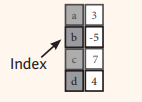
\includegraphics[keepaspectratio]{51.png}}

\begin{center}\rule{0.5\linewidth}{0.5pt}\end{center}

DataFrame

\pandocbounded{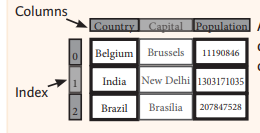
\includegraphics[keepaspectratio]{52.png}}

\begin{Shaded}
\begin{Highlighting}[]
\ImportTok{import}\NormalTok{ pandas }\ImportTok{as}\NormalTok{ pd}

\NormalTok{s }\OperatorTok{=}\NormalTok{ pd.Series([}\DecValTok{3}\NormalTok{, }\OperatorTok{{-}}\DecValTok{5}\NormalTok{, }\DecValTok{7}\NormalTok{, }\DecValTok{4}\NormalTok{])}
\BuiltInTok{print}\NormalTok{(s)}
\BuiltInTok{print}\NormalTok{(}\StringTok{"values"}\NormalTok{)}
\BuiltInTok{print}\NormalTok{(s.to\_numpy())}
\BuiltInTok{print}\NormalTok{(}\BuiltInTok{type}\NormalTok{(s.to\_numpy()))}
\BuiltInTok{print}\NormalTok{(s.index)}
\BuiltInTok{print}\NormalTok{(}\BuiltInTok{type}\NormalTok{(s.index))}
\end{Highlighting}
\end{Shaded}

\begin{verbatim}
0    3
1   -5
2    7
3    4
dtype: int64
values
[ 3 -5  7  4]
<class 'numpy.ndarray'>
RangeIndex(start=0, stop=4, step=1)
<class 'pandas.RangeIndex'>
\end{verbatim}

\begin{Shaded}
\begin{Highlighting}[]
\ImportTok{import}\NormalTok{ pandas }\ImportTok{as}\NormalTok{ pd}
\ImportTok{import}\NormalTok{ numpy }\ImportTok{as}\NormalTok{ np}

\NormalTok{s }\OperatorTok{=}\NormalTok{ pd.Series([}\DecValTok{3}\NormalTok{, }\OperatorTok{{-}}\DecValTok{5}\NormalTok{, }\DecValTok{7}\NormalTok{, }\DecValTok{4}\NormalTok{], index}\OperatorTok{=}\NormalTok{[}\StringTok{\textquotesingle{}a\textquotesingle{}}\NormalTok{, }\StringTok{\textquotesingle{}b\textquotesingle{}}\NormalTok{, }\StringTok{\textquotesingle{}c\textquotesingle{}}\NormalTok{, }\StringTok{\textquotesingle{}d\textquotesingle{}}\NormalTok{])}
\BuiltInTok{print}\NormalTok{(s)}
\BuiltInTok{print}\NormalTok{(s[}\StringTok{\textquotesingle{}b\textquotesingle{}}\NormalTok{])}
\NormalTok{s[}\StringTok{\textquotesingle{}b\textquotesingle{}}\NormalTok{] }\OperatorTok{=} \DecValTok{8}
\BuiltInTok{print}\NormalTok{(s)}
\BuiltInTok{print}\NormalTok{(s[s }\OperatorTok{\textgreater{}} \DecValTok{5}\NormalTok{])}
\BuiltInTok{print}\NormalTok{(s }\OperatorTok{*} \DecValTok{2}\NormalTok{)}
\BuiltInTok{print}\NormalTok{(np.sin(s))}
\end{Highlighting}
\end{Shaded}

\begin{verbatim}
a    3
b   -5
c    7
d    4
dtype: int64
-5
a    3
b    8
c    7
d    4
dtype: int64
b    8
c    7
dtype: int64
a     6
b    16
c    14
d     8
dtype: int64
a    0.141120
b    0.989358
c    0.656987
d   -0.756802
dtype: float64
\end{verbatim}

\begin{Shaded}
\begin{Highlighting}[]
\ImportTok{import}\NormalTok{ pandas }\ImportTok{as}\NormalTok{ pd}

\NormalTok{d }\OperatorTok{=}\NormalTok{ \{}\StringTok{\textquotesingle{}key1\textquotesingle{}}\NormalTok{: }\DecValTok{350}\NormalTok{, }\StringTok{\textquotesingle{}key2\textquotesingle{}}\NormalTok{: }\DecValTok{700}\NormalTok{, }\StringTok{\textquotesingle{}key3\textquotesingle{}}\NormalTok{: }\DecValTok{70}\NormalTok{\}}
\NormalTok{s }\OperatorTok{=}\NormalTok{ pd.Series(d)}
\BuiltInTok{print}\NormalTok{(s)}
\end{Highlighting}
\end{Shaded}

\begin{verbatim}
key1    350
key2    700
key3     70
dtype: int64
\end{verbatim}

\begin{Shaded}
\begin{Highlighting}[]
\ImportTok{import}\NormalTok{ pandas }\ImportTok{as}\NormalTok{ pd}

\NormalTok{d }\OperatorTok{=}\NormalTok{ \{}\StringTok{\textquotesingle{}key1\textquotesingle{}}\NormalTok{: }\DecValTok{350}\NormalTok{, }\StringTok{\textquotesingle{}key2\textquotesingle{}}\NormalTok{: }\DecValTok{700}\NormalTok{, }\StringTok{\textquotesingle{}key3\textquotesingle{}}\NormalTok{: }\DecValTok{70}\NormalTok{\}}
\NormalTok{k }\OperatorTok{=}\NormalTok{ [}\StringTok{\textquotesingle{}key0\textquotesingle{}}\NormalTok{, }\StringTok{\textquotesingle{}key2\textquotesingle{}}\NormalTok{, }\StringTok{\textquotesingle{}key3\textquotesingle{}}\NormalTok{, }\StringTok{\textquotesingle{}key1\textquotesingle{}}\NormalTok{]}
\NormalTok{s }\OperatorTok{=}\NormalTok{ pd.Series(d, index}\OperatorTok{=}\NormalTok{k)}
\BuiltInTok{print}\NormalTok{(s)}
\NormalTok{s.name }\OperatorTok{=} \StringTok{"Value"}
\NormalTok{s.index.name }\OperatorTok{=} \StringTok{"Key"}
\BuiltInTok{print}\NormalTok{(s)}
\end{Highlighting}
\end{Shaded}

\begin{verbatim}
key0      NaN
key2    700.0
key3     70.0
key1    350.0
dtype: float64
Key
key0      NaN
key2    700.0
key3     70.0
key1    350.0
Name: Value, dtype: float64
\end{verbatim}

\begin{Shaded}
\begin{Highlighting}[]
\ImportTok{import}\NormalTok{ pandas }\ImportTok{as}\NormalTok{ pd}

\NormalTok{data }\OperatorTok{=}\NormalTok{ \{}\StringTok{\textquotesingle{}Country\textquotesingle{}}\NormalTok{: [}\StringTok{\textquotesingle{}Belgium\textquotesingle{}}\NormalTok{, }\StringTok{\textquotesingle{}India\textquotesingle{}}\NormalTok{, }\StringTok{\textquotesingle{}Brazil\textquotesingle{}}\NormalTok{],}
        \StringTok{\textquotesingle{}Capital\textquotesingle{}}\NormalTok{: [}\StringTok{\textquotesingle{}Brussels\textquotesingle{}}\NormalTok{, }\StringTok{\textquotesingle{}New Delhi\textquotesingle{}}\NormalTok{, }\StringTok{\textquotesingle{}Brasília\textquotesingle{}}\NormalTok{],}
        \StringTok{\textquotesingle{}Population\textquotesingle{}}\NormalTok{: [}\DecValTok{11190846}\NormalTok{, }\DecValTok{1303171035}\NormalTok{, }\DecValTok{207847528}\NormalTok{]\}}
\NormalTok{frame }\OperatorTok{=}\NormalTok{ pd.DataFrame(data)}
\BuiltInTok{print}\NormalTok{(frame)}
\NormalTok{data2 }\OperatorTok{=}\NormalTok{ pd.DataFrame(data, columns}\OperatorTok{=}\NormalTok{[}\StringTok{\textquotesingle{}Country\textquotesingle{}}\NormalTok{, }\StringTok{\textquotesingle{}Population\textquotesingle{}}\NormalTok{, }\StringTok{\textquotesingle{}Capital\textquotesingle{}}\NormalTok{])}
\BuiltInTok{print}\NormalTok{(data2)}
\end{Highlighting}
\end{Shaded}

\begin{verbatim}
   Country    Capital  Population
0  Belgium   Brussels    11190846
1    India  New Delhi  1303171035
2   Brazil   Brasília   207847528
   Country  Population    Capital
0  Belgium    11190846   Brussels
1    India  1303171035  New Delhi
2   Brazil   207847528   Brasília
\end{verbatim}

\begin{Shaded}
\begin{Highlighting}[]
\ImportTok{import}\NormalTok{ pandas }\ImportTok{as}\NormalTok{ pd}

\NormalTok{data }\OperatorTok{=}\NormalTok{ \{}\StringTok{\textquotesingle{}Country\textquotesingle{}}\NormalTok{: [}\StringTok{\textquotesingle{}Belgium\textquotesingle{}}\NormalTok{, }\StringTok{\textquotesingle{}India\textquotesingle{}}\NormalTok{, }\StringTok{\textquotesingle{}Brazil\textquotesingle{}}\NormalTok{],}
        \StringTok{\textquotesingle{}Capital\textquotesingle{}}\NormalTok{: [}\StringTok{\textquotesingle{}Brussels\textquotesingle{}}\NormalTok{, }\StringTok{\textquotesingle{}New Delhi\textquotesingle{}}\NormalTok{, }\StringTok{\textquotesingle{}Brasília\textquotesingle{}}\NormalTok{],}
        \StringTok{\textquotesingle{}Population\textquotesingle{}}\NormalTok{: [}\DecValTok{11190846}\NormalTok{, }\DecValTok{1303171035}\NormalTok{, }\DecValTok{207847528}\NormalTok{]\}}
\NormalTok{df\_data }\OperatorTok{=}\NormalTok{ pd.DataFrame(data, columns}\OperatorTok{=}\NormalTok{[}\StringTok{\textquotesingle{}Country\textquotesingle{}}\NormalTok{, }\StringTok{\textquotesingle{}Population\textquotesingle{}}\NormalTok{, }\StringTok{\textquotesingle{}Capital\textquotesingle{}}\NormalTok{])}
\BuiltInTok{print}\NormalTok{(}\StringTok{"Shape:"}\NormalTok{, df\_data.shape)}
\BuiltInTok{print}\NormalTok{(}\StringTok{"{-}{-}"}\NormalTok{)}
\BuiltInTok{print}\NormalTok{(}\StringTok{"Index:"}\NormalTok{, df\_data.index)}
\BuiltInTok{print}\NormalTok{(}\StringTok{"{-}{-}"}\NormalTok{)}
\BuiltInTok{print}\NormalTok{(}\StringTok{"columns:"}\NormalTok{, df\_data.columns)}
\BuiltInTok{print}\NormalTok{(}\StringTok{"{-}{-}"}\NormalTok{)}
\NormalTok{df\_data.info()}
\BuiltInTok{print}\NormalTok{(}\StringTok{"{-}{-}"}\NormalTok{)}
\BuiltInTok{print}\NormalTok{(df\_data.count())}
\end{Highlighting}
\end{Shaded}

\begin{verbatim}
Shape: (3, 3)
--
Index: RangeIndex(start=0, stop=3, step=1)
--
columns: Index(['Country', 'Population', 'Capital'], dtype='str')
--
<class 'pandas.DataFrame'>
RangeIndex: 3 entries, 0 to 2
Data columns (total 3 columns):
 #   Column      Non-Null Count  Dtype
---  ------      --------------  -----
 0   Country     3 non-null      str  
 1   Population  3 non-null      int64
 2   Capital     3 non-null      str  
dtypes: int64(1), str(2)
memory usage: 204.0 bytes
--
Country       3
Population    3
Capital       3
dtype: int64
\end{verbatim}

\chapter{Pandas - indexing}\label{pandas---indexing}

\begin{Shaded}
\begin{Highlighting}[]
\ImportTok{import}\NormalTok{ pandas }\ImportTok{as}\NormalTok{ pd}

\NormalTok{data }\OperatorTok{=}\NormalTok{ \{}\StringTok{\textquotesingle{}Country\textquotesingle{}}\NormalTok{: [}\StringTok{\textquotesingle{}Belgium\textquotesingle{}}\NormalTok{, }\StringTok{\textquotesingle{}India\textquotesingle{}}\NormalTok{, }\StringTok{\textquotesingle{}Brazil\textquotesingle{}}\NormalTok{],}
        \StringTok{\textquotesingle{}Capital\textquotesingle{}}\NormalTok{: [}\StringTok{\textquotesingle{}Brussels\textquotesingle{}}\NormalTok{, }\StringTok{\textquotesingle{}New Delhi\textquotesingle{}}\NormalTok{, }\StringTok{\textquotesingle{}Brasília\textquotesingle{}}\NormalTok{],}
        \StringTok{\textquotesingle{}Population\textquotesingle{}}\NormalTok{: [}\DecValTok{11190846}\NormalTok{, }\DecValTok{1303171035}\NormalTok{, }\DecValTok{207847528}\NormalTok{]\}}
\NormalTok{data2 }\OperatorTok{=}\NormalTok{ pd.DataFrame(data, columns}\OperatorTok{=}\NormalTok{[}\StringTok{\textquotesingle{}Country\textquotesingle{}}\NormalTok{, }\StringTok{\textquotesingle{}Population\textquotesingle{}}\NormalTok{, }\StringTok{\textquotesingle{}Capital\textquotesingle{}}\NormalTok{])}
\BuiltInTok{print}\NormalTok{(data2.iloc[[}\DecValTok{0}\NormalTok{], [}\DecValTok{0}\NormalTok{]])}
\BuiltInTok{print}\NormalTok{(}\StringTok{"{-}{-}"}\NormalTok{)}
\BuiltInTok{print}\NormalTok{(data2.loc[[}\DecValTok{0}\NormalTok{], [}\StringTok{\textquotesingle{}Country\textquotesingle{}}\NormalTok{]])}
\BuiltInTok{print}\NormalTok{(}\StringTok{"{-}{-}"}\NormalTok{)}
\BuiltInTok{print}\NormalTok{(data2.loc[}\DecValTok{2}\NormalTok{])}
\BuiltInTok{print}\NormalTok{(}\StringTok{"{-}{-}"}\NormalTok{)}
\BuiltInTok{print}\NormalTok{(data2.loc[:, }\StringTok{\textquotesingle{}Capital\textquotesingle{}}\NormalTok{])}
\BuiltInTok{print}\NormalTok{(}\StringTok{"{-}{-}"}\NormalTok{)}
\BuiltInTok{print}\NormalTok{(data2.loc[}\DecValTok{1}\NormalTok{, }\StringTok{\textquotesingle{}Capital\textquotesingle{}}\NormalTok{])}
\end{Highlighting}
\end{Shaded}

\begin{verbatim}
   Country
0  Belgium
--
   Country
0  Belgium
--
Country          Brazil
Population    207847528
Capital       Brasília
Name: 2, dtype: object
--
0     Brussels
1    New Delhi
2    Brasília
Name: Capital, dtype: str
--
New Delhi
\end{verbatim}

\begin{enumerate}
\def\labelenumi{\arabic{enumi}.}
\tightlist
\item
  \texttt{loc}:
\end{enumerate}

\begin{itemize}
\tightlist
\item
  This is a label-based indexing method, meaning it uses column label
  names and row indices to select data.
\item
  It works based on index labels and column labels, which allows for
  more convenient data filtering.
\item
  It supports both individual labels and label ranges.
\item
  It also works with non-numeric labels.
\item
  Example usage:
  \texttt{df.loc{[}1:3,\ {[}\textquotesingle{}A\textquotesingle{},\ \textquotesingle{}B\textquotesingle{}{]}{]}}
  - returns rows from index 1 to 3 (inclusive) and columns `A' and `B'.
\end{itemize}

\begin{enumerate}
\def\labelenumi{\arabic{enumi}.}
\setcounter{enumi}{1}
\tightlist
\item
  \texttt{iloc}:
\end{enumerate}

\begin{itemize}
\tightlist
\item
  This is a position-based indexing method, meaning it uses numeric
  column and row indices to select data.
\item
  It works based on numeric indices for both rows and columns.
\item
  It supports individual indices and index ranges.
\item
  When using index ranges, the range is half-open, meaning the right end
  is not included.
\item
  Example usage: \texttt{df.iloc{[}1:3,\ 0:2{]}} - returns rows from
  index 1 to 3 (excluding 3) and columns from index 0 to 2 (excluding
  2).
\end{itemize}

\begin{Shaded}
\begin{Highlighting}[]
\ImportTok{import}\NormalTok{ pandas }\ImportTok{as}\NormalTok{ pd}

\NormalTok{data }\OperatorTok{=}\NormalTok{ \{}\StringTok{\textquotesingle{}Country\textquotesingle{}}\NormalTok{: [}\StringTok{\textquotesingle{}Belgium\textquotesingle{}}\NormalTok{, }\StringTok{\textquotesingle{}India\textquotesingle{}}\NormalTok{, }\StringTok{\textquotesingle{}Brazil\textquotesingle{}}\NormalTok{],}
        \StringTok{\textquotesingle{}Capital\textquotesingle{}}\NormalTok{: [}\StringTok{\textquotesingle{}Brussels\textquotesingle{}}\NormalTok{, }\StringTok{\textquotesingle{}New Delhi\textquotesingle{}}\NormalTok{, }\StringTok{\textquotesingle{}Brasília\textquotesingle{}}\NormalTok{],}
        \StringTok{\textquotesingle{}Population\textquotesingle{}}\NormalTok{: [}\DecValTok{11190846}\NormalTok{, }\DecValTok{1303171035}\NormalTok{, }\DecValTok{207847528}\NormalTok{]\}}
\NormalTok{data2 }\OperatorTok{=}\NormalTok{ pd.DataFrame(data, columns}\OperatorTok{=}\NormalTok{[}\StringTok{\textquotesingle{}Country\textquotesingle{}}\NormalTok{, }\StringTok{\textquotesingle{}Population\textquotesingle{}}\NormalTok{, }\StringTok{\textquotesingle{}Capital\textquotesingle{}}\NormalTok{])}
\BuiltInTok{print}\NormalTok{(data2[}\StringTok{\textquotesingle{}Population\textquotesingle{}}\NormalTok{])}
\BuiltInTok{print}\NormalTok{(}\StringTok{"{-}{-}"}\NormalTok{)}
\BuiltInTok{print}\NormalTok{(data2[data2[}\StringTok{\textquotesingle{}Population\textquotesingle{}}\NormalTok{] }\OperatorTok{\textgreater{}} \DecValTok{1200000000}\NormalTok{])}
\BuiltInTok{print}\NormalTok{(}\StringTok{"{-}{-}"}\NormalTok{)}
\end{Highlighting}
\end{Shaded}

\begin{verbatim}
0      11190846
1    1303171035
2     207847528
Name: Population, dtype: int64
--
  Country  Population    Capital
1   India  1303171035  New Delhi
--
\end{verbatim}

\textbf{Exercises:} (\texttt{ex9.py})

Practice indexing on the data frame below (you don't need to use all
rows):

\begin{itemize}
\tightlist
\item
  \textbf{Categorical columns}:

  \begin{itemize}
  \tightlist
  \item
    \texttt{Region} -- sales region
  \item
    \texttt{Product} -- product type
  \item
    \texttt{Sales\_Channel} -- sales channel (online, retail store,
    wholesale)
  \end{itemize}
\item
  \textbf{Numeric columns}:

  \begin{itemize}
  \tightlist
  \item
    \texttt{Units\_Sold} -- number of units sold
  \item
    \texttt{Revenue} -- revenue in thousands of GBP
  \item
    \texttt{Profit} -- profit in thousands of GBP
  \end{itemize}
\end{itemize}

{\def\LTcaptype{none} % do not increment counter
\begin{longtable}[]{@{}
  >{\raggedright\arraybackslash}p{(\linewidth - 10\tabcolsep) * \real{0.1733}}
  >{\raggedright\arraybackslash}p{(\linewidth - 10\tabcolsep) * \real{0.2133}}
  >{\raggedright\arraybackslash}p{(\linewidth - 10\tabcolsep) * \real{0.2267}}
  >{\raggedright\arraybackslash}p{(\linewidth - 10\tabcolsep) * \real{0.1600}}
  >{\raggedright\arraybackslash}p{(\linewidth - 10\tabcolsep) * \real{0.1200}}
  >{\raggedright\arraybackslash}p{(\linewidth - 10\tabcolsep) * \real{0.1067}}@{}}
\toprule\noalign{}
\begin{minipage}[b]{\linewidth}\raggedright
Region
\end{minipage} & \begin{minipage}[b]{\linewidth}\raggedright
Product
\end{minipage} & \begin{minipage}[b]{\linewidth}\raggedright
Sales\_Channel
\end{minipage} & \begin{minipage}[b]{\linewidth}\raggedright
Units\_Sold
\end{minipage} & \begin{minipage}[b]{\linewidth}\raggedright
Revenue
\end{minipage} & \begin{minipage}[b]{\linewidth}\raggedright
Profit
\end{minipage} \\
\midrule\noalign{}
\endhead
\bottomrule\noalign{}
\endlastfoot
North & Electronics & Online & 120 & 60.5 & 15.2 \\
South & Furniture & Retail & 80 & 45.0 & 12.0 \\
East & Clothing & Online & 200 & 35.0 & 8.5 \\
West & Electronics & Wholesale & 150 & 70.0 & 20.5 \\
North & Furniture & Retail & 90 & 50.5 & 13.2 \\
South & Clothing & Online & 300 & 55.0 & 10.0 \\
East & Electronics & Retail & 110 & 62.0 & 16.0 \\
West & Furniture & Online & 70 & 30.0 & 7.5 \\
North & Clothing & Wholesale & 250 & 40.0 & 9.0 \\
South & Electronics & Retail & 130 & 75.0 & 22.0 \\
\end{longtable}
}

\chapter{Loading data}\label{loading-data}

\section{Handling csv files}\label{handling-csv-files}

The \texttt{pandas.read\_csv} function

Documentation:
\href{https://pandas.pydata.org/pandas-docs/stable/reference/api/pandas.read_csv.html}{link}

Selected arguments:

\begin{itemize}
\tightlist
\item
  \texttt{filepath} - access path
\item
  \texttt{sep=\_NoDefault.no\_default,\ delimiter=None} - separator
\item
  \texttt{header=\textquotesingle{}infer\textquotesingle{}} - header -
  by default the column names, alternatively \texttt{header=None} means
  no header
\item
  \texttt{index\_col=None} - sets a column as the index (row names)
\item
  \texttt{thousands=None} - thousands separator
\item
  \texttt{decimal=\textquotesingle{}.\textquotesingle{}} - decimal
  separator
\end{itemize}

Saving with \texttt{pandas.DataFrame.to\_csv}

Documentation:
\href{https://pandas.pydata.org/pandas-docs/stable/reference/api/pandas.DataFrame.to_csv.html}{link}

\section{Handling Excel files}\label{handling-excel-files}

The \texttt{pandas.read\_excel} function

\url{https://pandas.pydata.org/docs/reference/api/pandas.read_excel.html}

** Important: you need to install the \texttt{openpyxl} library to
import .xlsx files and \texttt{xlrd} to import .xls files (in most cases
you don't need to import them explicitly in the code)

Selected arguments:

\begin{itemize}
\tightlist
\item
  \texttt{io} - access path
\item
  \texttt{sheet\_name=0} - sheet name
\item
  \texttt{header=\textquotesingle{}infer\textquotesingle{}} - header -
  by default the column names, alternatively \texttt{header=None} means
  no header
\item
  \texttt{index\_col=None} - sets a column as the index (row names)
\item
  \texttt{thousands=None} - thousands separator
\item
  \texttt{decimal=\textquotesingle{}.\textquotesingle{}} - decimal
  separator
\end{itemize}

\section{\texorpdfstring{Handling
\texttt{sqllite3}}{Handling sqllite3}}\label{handling-sqllite3}

\begin{Shaded}
\begin{Highlighting}[]
\ImportTok{import}\NormalTok{ pandas }\ImportTok{as}\NormalTok{ pd}
\ImportTok{from}\NormalTok{ sqlite3 }\ImportTok{import} \ExtensionTok{connect}

\NormalTok{conn }\OperatorTok{=} \ExtensionTok{connect}\NormalTok{(}\StringTok{\textquotesingle{}sales\_data2.db\textquotesingle{}}\NormalTok{)}
\NormalTok{data }\OperatorTok{=}\NormalTok{ pd.read\_sql(}\StringTok{"SELECT * FROM sales\_data"}\NormalTok{, con}\OperatorTok{=}\NormalTok{conn)}
\end{Highlighting}
\end{Shaded}

\section{Sample files for exercises}\label{sample-files-for-exercises}

\url{https://github.com/pjastr/DAV-files}

\chapter{Pandas - sorting}\label{pandas---sorting}

\begin{Shaded}
\begin{Highlighting}[]
\ImportTok{import}\NormalTok{ pandas }\ImportTok{as}\NormalTok{ pd}

\CommentTok{\# Sample data frame}
\NormalTok{data }\OperatorTok{=}\NormalTok{ pd.DataFrame(\{}
    \StringTok{\textquotesingle{}Name\textquotesingle{}}\NormalTok{: [}\StringTok{\textquotesingle{}Alice\textquotesingle{}}\NormalTok{, }\StringTok{\textquotesingle{}Tom\textquotesingle{}}\NormalTok{, }\StringTok{\textquotesingle{}Charlie\textquotesingle{}}\NormalTok{],}
    \StringTok{\textquotesingle{}Age\textquotesingle{}}\NormalTok{: [}\DecValTok{25}\NormalTok{, }\DecValTok{42}\NormalTok{, }\DecValTok{35}\NormalTok{],}
    \StringTok{\textquotesingle{}Salary\textquotesingle{}}\NormalTok{: [}\DecValTok{50000}\NormalTok{, }\DecValTok{60000}\NormalTok{, }\DecValTok{70000}\NormalTok{]}
\NormalTok{\})}

\CommentTok{\# Sorting by the \textquotesingle{}Age\textquotesingle{} column}
\NormalTok{s1 }\OperatorTok{=}\NormalTok{ data.sort\_values(by}\OperatorTok{=}\StringTok{\textquotesingle{}Age\textquotesingle{}}\NormalTok{)}
\BuiltInTok{print}\NormalTok{(s1)}
\CommentTok{\# Sorting in reverse order}
\NormalTok{s2 }\OperatorTok{=}\NormalTok{ data.sort\_values(by}\OperatorTok{=}\StringTok{\textquotesingle{}Salary\textquotesingle{}}\NormalTok{, ascending}\OperatorTok{=}\VariableTok{False}\NormalTok{)}
\BuiltInTok{print}\NormalTok{(s2)}
\CommentTok{\# Sorting by \textquotesingle{}Age\textquotesingle{} ascending, then \textquotesingle{}Salary\textquotesingle{} descending}
\NormalTok{s3 }\OperatorTok{=}\NormalTok{ data.sort\_values(by}\OperatorTok{=}\NormalTok{[}\StringTok{\textquotesingle{}Age\textquotesingle{}}\NormalTok{, }\StringTok{\textquotesingle{}Salary\textquotesingle{}}\NormalTok{], ascending}\OperatorTok{=}\NormalTok{[}\VariableTok{True}\NormalTok{, }\VariableTok{False}\NormalTok{])}
\BuiltInTok{print}\NormalTok{(s3)}
\end{Highlighting}
\end{Shaded}

\begin{verbatim}
      Name  Age  Salary
0    Alice   25   50000
2  Charlie   35   70000
1      Tom   42   60000
      Name  Age  Salary
2  Charlie   35   70000
1      Tom   42   60000
0    Alice   25   50000
      Name  Age  Salary
0    Alice   25   50000
2  Charlie   35   70000
1      Tom   42   60000
\end{verbatim}

\begin{Shaded}
\begin{Highlighting}[]
\ImportTok{import}\NormalTok{ pandas }\ImportTok{as}\NormalTok{ pd}

\CommentTok{\# Sample data frame}
\NormalTok{data }\OperatorTok{=}\NormalTok{ pd.DataFrame(\{}
    \StringTok{\textquotesingle{}Name\textquotesingle{}}\NormalTok{: [}\StringTok{\textquotesingle{}Alice\textquotesingle{}}\NormalTok{, }\StringTok{\textquotesingle{}Tom\textquotesingle{}}\NormalTok{, }\StringTok{\textquotesingle{}Charlie\textquotesingle{}}\NormalTok{],}
    \StringTok{\textquotesingle{}Age\textquotesingle{}}\NormalTok{: [}\DecValTok{25}\NormalTok{, }\DecValTok{41}\NormalTok{, }\DecValTok{35}\NormalTok{],}
    \StringTok{\textquotesingle{}Salary\textquotesingle{}}\NormalTok{: [}\DecValTok{50000}\NormalTok{, }\DecValTok{60000}\NormalTok{, }\DecValTok{70000}\NormalTok{]}
\NormalTok{\})}

\CommentTok{\# Inplace sorting (replacing the existing variable) {-} currently not recommended}
\NormalTok{data.sort\_values(by}\OperatorTok{=}\StringTok{\textquotesingle{}Age\textquotesingle{}}\NormalTok{, inplace}\OperatorTok{=}\VariableTok{True}\NormalTok{)}
\BuiltInTok{print}\NormalTok{(data)}
\end{Highlighting}
\end{Shaded}

\begin{verbatim}
      Name  Age  Salary
0    Alice   25   50000
2  Charlie   35   70000
1      Tom   41   60000
\end{verbatim}

\begin{Shaded}
\begin{Highlighting}[]
\ImportTok{import}\NormalTok{ pandas }\ImportTok{as}\NormalTok{ pd}

\NormalTok{df2 }\OperatorTok{=}\NormalTok{ pd.DataFrame(\{}
    \StringTok{\textquotesingle{}Name\textquotesingle{}}\NormalTok{: [}\StringTok{\textquotesingle{}Alice\textquotesingle{}}\NormalTok{, }\StringTok{\textquotesingle{}Bob\textquotesingle{}}\NormalTok{, }\StringTok{\textquotesingle{}Charlie\textquotesingle{}}\NormalTok{, }\StringTok{\textquotesingle{}Dave\textquotesingle{}}\NormalTok{],}
    \StringTok{\textquotesingle{}Age\textquotesingle{}}\NormalTok{: [}\DecValTok{25}\NormalTok{, }\DecValTok{30}\NormalTok{, }\VariableTok{None}\NormalTok{, }\DecValTok{35}\NormalTok{],}
    \StringTok{\textquotesingle{}Salary\textquotesingle{}}\NormalTok{: [}\DecValTok{50000}\NormalTok{, }\VariableTok{None}\NormalTok{, }\DecValTok{70000}\NormalTok{, }\DecValTok{60000}\NormalTok{]}
\NormalTok{\})}

\CommentTok{\# Sorting with NaN at the end}
\NormalTok{s2 }\OperatorTok{=}\NormalTok{ df2.sort\_values(by}\OperatorTok{=}\StringTok{\textquotesingle{}Age\textquotesingle{}}\NormalTok{, na\_position}\OperatorTok{=}\StringTok{\textquotesingle{}last\textquotesingle{}}\NormalTok{)}
\BuiltInTok{print}\NormalTok{(s2)}
\CommentTok{\# Sorting with NaN at the beginning}
\NormalTok{s3 }\OperatorTok{=}\NormalTok{ df2.sort\_values(by}\OperatorTok{=}\StringTok{\textquotesingle{}Age\textquotesingle{}}\NormalTok{, na\_position}\OperatorTok{=}\StringTok{\textquotesingle{}first\textquotesingle{}}\NormalTok{)}
\BuiltInTok{print}\NormalTok{(s3)}
\end{Highlighting}
\end{Shaded}

\begin{verbatim}
      Name   Age   Salary
0    Alice  25.0  50000.0
1      Bob  30.0      NaN
3     Dave  35.0  60000.0
2  Charlie   NaN  70000.0
      Name   Age   Salary
2  Charlie   NaN  70000.0
0    Alice  25.0  50000.0
1      Bob  30.0      NaN
3     Dave  35.0  60000.0
\end{verbatim}

\begin{Shaded}
\begin{Highlighting}[]
\ImportTok{import}\NormalTok{ pandas }\ImportTok{as}\NormalTok{ pd}

\NormalTok{df3 }\OperatorTok{=}\NormalTok{ pd.DataFrame(\{}
    \StringTok{\textquotesingle{}Name\textquotesingle{}}\NormalTok{: [}\StringTok{\textquotesingle{}Alice\textquotesingle{}}\NormalTok{, }\StringTok{\textquotesingle{}Bob\textquotesingle{}}\NormalTok{, }\StringTok{\textquotesingle{}Charlie\textquotesingle{}}\NormalTok{, }\StringTok{\textquotesingle{}Dave\textquotesingle{}}\NormalTok{],}
    \StringTok{\textquotesingle{}Age\textquotesingle{}}\NormalTok{: [}\DecValTok{25}\NormalTok{, }\DecValTok{30}\NormalTok{, }\VariableTok{None}\NormalTok{, }\DecValTok{35}\NormalTok{],}
    \StringTok{\textquotesingle{}Salary\textquotesingle{}}\NormalTok{: [}\DecValTok{50000}\NormalTok{, }\VariableTok{None}\NormalTok{, }\DecValTok{70000}\NormalTok{, }\DecValTok{60000}\NormalTok{]}
\NormalTok{\})}

\NormalTok{s3 }\OperatorTok{=}\NormalTok{ df3.sort\_values(by}\OperatorTok{=}\StringTok{\textquotesingle{}Name\textquotesingle{}}\NormalTok{, key}\OperatorTok{=}\KeywordTok{lambda}\NormalTok{ x: x.}\BuiltInTok{str}\NormalTok{.}\BuiltInTok{len}\NormalTok{())}
\BuiltInTok{print}\NormalTok{(s3)}
\end{Highlighting}
\end{Shaded}

\begin{verbatim}
      Name   Age   Salary
1      Bob  30.0      NaN
3     Dave  35.0  60000.0
0    Alice  25.0  50000.0
2  Charlie   NaN  70000.0
\end{verbatim}

\chapter{Pandas - time series}\label{pandas---time-series}

Converting a string to \texttt{datetime} format (date-time)

\begin{Shaded}
\begin{Highlighting}[]
\ImportTok{import}\NormalTok{ pandas }\ImportTok{as}\NormalTok{ pd}

\NormalTok{data }\OperatorTok{=}\NormalTok{ \{}\StringTok{\textquotesingle{}date\textquotesingle{}}\NormalTok{: [}\StringTok{\textquotesingle{}2023{-}01{-}01\textquotesingle{}}\NormalTok{, }\StringTok{\textquotesingle{}2023{-}01{-}02\textquotesingle{}}\NormalTok{, }\StringTok{\textquotesingle{}2023{-}01{-}03\textquotesingle{}}\NormalTok{], }\StringTok{\textquotesingle{}value\textquotesingle{}}\NormalTok{: [}\DecValTok{10}\NormalTok{, }\DecValTok{15}\NormalTok{, }\DecValTok{20}\NormalTok{]\}}
\NormalTok{data\_frame }\OperatorTok{=}\NormalTok{ pd.DataFrame(data)}
\NormalTok{data\_frame[}\StringTok{\textquotesingle{}date\textquotesingle{}}\NormalTok{] }\OperatorTok{=}\NormalTok{ pd.to\_datetime(data\_frame[}\StringTok{\textquotesingle{}date\textquotesingle{}}\NormalTok{])}
\BuiltInTok{print}\NormalTok{(data)}
\end{Highlighting}
\end{Shaded}

\begin{verbatim}
{'date': ['2023-01-01', '2023-01-02', '2023-01-03'], 'value': [10, 15, 20]}
\end{verbatim}

The \texttt{errors} argument in the \texttt{pd.to\_datetime} function
controls how the function should behave when it encounters invalid data
while attempting to convert values into \texttt{datetime} objects.
Possible values for \texttt{errors} are:

\begin{enumerate}
\def\labelenumi{\arabic{enumi}.}
\tightlist
\item
  \textbf{\texttt{\textquotesingle{}raise\textquotesingle{}}} (default):
  Raises an exception if it encounters an invalid data format.
\item
  \textbf{\texttt{\textquotesingle{}coerce\textquotesingle{}}}: Replaces
  invalid values with \texttt{NaT} (Not a Time).
\item
  \textbf{\texttt{\textquotesingle{}ignore\textquotesingle{}}}: Returns
  the input data unchanged when it encounters an error (option
  deprecated in later versions).
\end{enumerate}

Code to paste into the environment:

\begin{Shaded}
\begin{Highlighting}[]
\ImportTok{import}\NormalTok{ pandas }\ImportTok{as}\NormalTok{ pd}

\NormalTok{data }\OperatorTok{=}\NormalTok{ \{}\StringTok{\textquotesingle{}date\textquotesingle{}}\NormalTok{: [}\StringTok{\textquotesingle{}2023{-}01{-}01\textquotesingle{}}\NormalTok{, }\StringTok{\textquotesingle{}invalid\textquotesingle{}}\NormalTok{, }\StringTok{\textquotesingle{}2023{-}01{-}03\textquotesingle{}}\NormalTok{], }\StringTok{\textquotesingle{}value\textquotesingle{}}\NormalTok{: [}\DecValTok{10}\NormalTok{, }\DecValTok{15}\NormalTok{, }\DecValTok{20}\NormalTok{]\}}
\NormalTok{data\_frame }\OperatorTok{=}\NormalTok{ pd.DataFrame(data)}
\NormalTok{data\_frame[}\StringTok{\textquotesingle{}date\textquotesingle{}}\NormalTok{] }\OperatorTok{=}\NormalTok{ pd.to\_datetime(data\_frame[}\StringTok{\textquotesingle{}date\textquotesingle{}}\NormalTok{], errors}\OperatorTok{=}\StringTok{\textquotesingle{}ignore\textquotesingle{}}\NormalTok{)}
\end{Highlighting}
\end{Shaded}

The \texttt{format} argument in the \texttt{pandas.to\_datetime}
function allows you to specify the exact date and time format to be used
for parsing input values. This is useful when input data has a fixed,
specific format, which can speed up processing and reduce the risk of
misinterpreting dates.

\begin{Shaded}
\begin{Highlighting}[]
\ImportTok{import}\NormalTok{ pandas }\ImportTok{as}\NormalTok{ pd}

\CommentTok{\# Sample input data with different formats}
\NormalTok{data1 }\OperatorTok{=}\NormalTok{ [}\StringTok{\textquotesingle{}01{-}01{-}2025\textquotesingle{}}\NormalTok{, }\StringTok{\textquotesingle{}15{-}03{-}2025\textquotesingle{}}\NormalTok{, }\StringTok{\textquotesingle{}30{-}12{-}2025\textquotesingle{}}\NormalTok{]  }\CommentTok{\# Format: DD{-}MM{-}YYYY}
\NormalTok{data2 }\OperatorTok{=}\NormalTok{ [}\StringTok{\textquotesingle{}2025/01/01\textquotesingle{}}\NormalTok{, }\StringTok{\textquotesingle{}2025/03/15\textquotesingle{}}\NormalTok{, }\StringTok{\textquotesingle{}2025/12/30\textquotesingle{}}\NormalTok{]  }\CommentTok{\# Format: YYYY/MM/DD}

\CommentTok{\# Conversion with a specified format (DD{-}MM{-}YYYY)}
\NormalTok{df1 }\OperatorTok{=}\NormalTok{ pd.DataFrame(data1)}
\NormalTok{df1[}\DecValTok{0}\NormalTok{] }\OperatorTok{=}\NormalTok{ pd.to\_datetime(df1[}\DecValTok{0}\NormalTok{], }\BuiltInTok{format}\OperatorTok{=}\StringTok{\textquotesingle{}}\SpecialCharTok{\%d}\StringTok{{-}\%m{-}\%Y\textquotesingle{}}\NormalTok{)}
\BuiltInTok{print}\NormalTok{(}\StringTok{"Conversion with format \textquotesingle{}}\SpecialCharTok{\%d}\StringTok{{-}\%m{-}\%Y\textquotesingle{}:"}\NormalTok{)}
\BuiltInTok{print}\NormalTok{(df1)}

\CommentTok{\# Conversion with a specified format (YYYY/MM/DD)}
\NormalTok{df2 }\OperatorTok{=}\NormalTok{ pd.DataFrame(data2)}
\NormalTok{df2[}\DecValTok{0}\NormalTok{] }\OperatorTok{=}\NormalTok{ pd.to\_datetime(df2[}\DecValTok{0}\NormalTok{], }\BuiltInTok{format}\OperatorTok{=}\StringTok{\textquotesingle{}\%Y/\%m/}\SpecialCharTok{\%d}\StringTok{\textquotesingle{}}\NormalTok{)}
\BuiltInTok{print}\NormalTok{(}\StringTok{"}\CharTok{\textbackslash{}n}\StringTok{Conversion with format \textquotesingle{}\%Y/\%m/}\SpecialCharTok{\%d}\StringTok{\textquotesingle{}:"}\NormalTok{)}
\BuiltInTok{print}\NormalTok{(df2)}
\end{Highlighting}
\end{Shaded}

\begin{verbatim}
Conversion with format '%d-%m-%Y':
           0
0 2025-01-01
1 2025-03-15
2 2025-12-30

Conversion with format '%Y/%m/%d':
           0
0 2025-01-01
1 2025-03-15
2 2025-12-30
\end{verbatim}

{\def\LTcaptype{none} % do not increment counter
\begin{longtable}[]{@{}
  >{\raggedright\arraybackslash}p{(\linewidth - 4\tabcolsep) * \real{0.1884}}
  >{\raggedright\arraybackslash}p{(\linewidth - 4\tabcolsep) * \real{0.4928}}
  >{\raggedright\arraybackslash}p{(\linewidth - 4\tabcolsep) * \real{0.3188}}@{}}
\toprule\noalign{}
\begin{minipage}[b]{\linewidth}\raggedright
Format code
\end{minipage} & \begin{minipage}[b]{\linewidth}\raggedright
Description
\end{minipage} & \begin{minipage}[b]{\linewidth}\raggedright
Example
\end{minipage} \\
\midrule\noalign{}
\endhead
\bottomrule\noalign{}
\endlastfoot
\texttt{\%Y} & Year in 4-digit format & 2025 \\
\texttt{\%y} & Year in 2-digit format & 25 \\
\texttt{\%m} & Month (digits, 2-digit) & 01 (January), 12 (December) \\
\texttt{\%d} & Day of the month (2-digit) & 01, 15, 31 \\
\texttt{\%B} & Full month name & January, December \\
\texttt{\%b} & Abbreviated month name & Jan, Dec \\
\texttt{\%A} & Full weekday name & Monday, Sunday \\
\texttt{\%a} & Abbreviated weekday name & Mon, Sun \\
\texttt{\%H} & Hour in 24-hour format & 00, 12, 23 \\
\texttt{\%I} & Hour in 12-hour format & 01, 11 \\
\texttt{\%p} & AM/PM & AM, PM \\
\texttt{\%M} & Minutes & 00, 30, 59 \\
\texttt{\%S} & Seconds & 00, 30, 59 \\
\end{longtable}
}

Polish month names in nominative or abbreviated form.

Note: That isn't grammatically correct. Traditional format (DMY):
dd.mm.yyyy, often with dots as separators; the more official form is d
yyyy, or, less frequently, d yyyy. Official format (YMD): the ISO 8601
YYYY-MM-DD format is used in Poland in official documents, banks,
computer systems, and on the internet.

\begin{Shaded}
\begin{Highlighting}[]
\ImportTok{import}\NormalTok{ locale}
\ImportTok{import}\NormalTok{ pandas }\ImportTok{as}\NormalTok{ pd}

\NormalTok{locale.setlocale(locale.LC\_ALL, }\StringTok{\textquotesingle{}PL\textquotesingle{}}\NormalTok{)}
\CommentTok{\# locale.setlocale(locale.LC\_TIME, \textquotesingle{}pl\_PL.UTF{-}8\textquotesingle{})  \# On Linux/Mac systems}
\CommentTok{\# locale.setlocale(locale.LC\_TIME, \textquotesingle{}Polish\_Poland.1250\textquotesingle{})  \# On Windows}

\NormalTok{data }\OperatorTok{=}\NormalTok{ [}\StringTok{\textquotesingle{}10 styczeń 2025\textquotesingle{}}\NormalTok{, }\StringTok{\textquotesingle{}15 grudzień 2025\textquotesingle{}}\NormalTok{, }\StringTok{\textquotesingle{}5 marzec 2025\textquotesingle{}}\NormalTok{]}
\NormalTok{data\_frame }\OperatorTok{=}\NormalTok{ pd.DataFrame(data)}
\NormalTok{data\_frame[}\DecValTok{0}\NormalTok{] }\OperatorTok{=}\NormalTok{ pd.to\_datetime(data\_frame[}\DecValTok{0}\NormalTok{], }\BuiltInTok{format}\OperatorTok{=}\StringTok{\textquotesingle{}}\SpecialCharTok{\%d}\StringTok{ \%B \%Y\textquotesingle{}}\NormalTok{)}
\BuiltInTok{print}\NormalTok{(data\_frame)}
\NormalTok{data2 }\OperatorTok{=}\NormalTok{ [}\StringTok{\textquotesingle{}10 sty 2025\textquotesingle{}}\NormalTok{, }\StringTok{\textquotesingle{}15 gru 2025\textquotesingle{}}\NormalTok{, }\StringTok{\textquotesingle{}5 mar 2025\textquotesingle{}}\NormalTok{]}
\NormalTok{df2 }\OperatorTok{=}\NormalTok{ pd.DataFrame(data2)}
\NormalTok{df2[}\DecValTok{0}\NormalTok{] }\OperatorTok{=}\NormalTok{ pd.to\_datetime(df2[}\DecValTok{0}\NormalTok{], }\BuiltInTok{format}\OperatorTok{=}\StringTok{\textquotesingle{}}\SpecialCharTok{\%d}\StringTok{ \%b \%Y\textquotesingle{}}\NormalTok{)}
\BuiltInTok{print}\NormalTok{(df2)}
\end{Highlighting}
\end{Shaded}

\begin{verbatim}
           0
0 2025-01-10
1 2025-12-15
2 2025-03-05
           0
0 2025-01-10
1 2025-12-15
2 2025-03-05
\end{verbatim}

\textbf{Exercise:} (\texttt{extime.py})

Load the following files and transform the date column:

\begin{itemize}
\item
  date\_sale.csv
\item
  date\_temp.csv
\end{itemize}

Hint:

\begin{Shaded}
\begin{Highlighting}[]
\ImportTok{import}\NormalTok{ pandas }\ImportTok{as}\NormalTok{ pd}

\NormalTok{data }\OperatorTok{=}\NormalTok{ pd.read\_csv(}\StringTok{"date\_sale.csv"}\NormalTok{, parse\_dates}\OperatorTok{=}\NormalTok{[}\StringTok{"Sale\_Date"}\NormalTok{], date\_format}\OperatorTok{=}\StringTok{"}\SpecialCharTok{\%d}\StringTok{{-}\%m{-}\%Y"}\NormalTok{)}
\end{Highlighting}
\end{Shaded}





\end{document}
